%% thesis.tex – IITM 2022 template (M.Tech, Industrial AI)
\overfullrule=5pt
\documentclass[mtech,smplmath]{iitmdissertation}
\usepackage{float}
\PassOptionsToPackage{hyphens}{url} % BEFORE hyperref
\usepackage[hidelinks]{hyperref}
\usepackage{doi}
\usepackage{xurl}     % extends URL breaking
\urlstyle{same}
\AtBeginDocument{%
  \pdfstringdefDisableCommands{%
    \let\MakeUppercase\relax
  }%
}
\usepackage{textcomp}
\usepackage{algorithm}
\usepackage{algorithmic}
\usepackage{cleveref}  % Optional: \Cref{sec:foo}
\usepackage{array} % you already seem to use this for >{\raggedright\arraybackslash}
\usepackage{caption}    % for \captionof outside floats (not needed here, but good to have)
\usepackage{placeins}
\usepackage{scrhack}
\usepackage{pgfplots}
\pgfplotsset{compat=1.18}
\usepackage{multirow}
\usepackage{graphicx}
\usepackage{tikz,pgfplots}
\usetikzlibrary{fit,positioning}
\usetikzlibrary{arrows.meta, positioning, calc, shapes.geometric, bending}
\usetikzlibrary{decorations.pathmorphing}


\tikzset{
  block/.style={
    draw,
    rectangle,
    rounded corners,
    minimum height=1.0cm,
    minimum width=3.4cm,
    align=center,
    font=\small
  },
  smallblock/.style={
    draw,
    rectangle,
    rounded corners,
    minimum height=0.9cm,
    minimum width=3.6cm,
    align=center,
    font=\footnotesize
  },
  arrow/.style={
    -{Latex[length=3mm,width=2mm]},thick}
}
\usepackage{siunitx}
%\usepackage{wasysym}  % for \rupee

% ==============================================================================
% CUSTOM MATH OPERATORS & SYMBOLS FOR THE ENTIRE THESIS
% ==============================================================================
\usepackage{tabularx}
\usepackage{amsmath,amssymb}   % already loaded – needed for \DeclareMathOperator etc.
\usepackage{booktabs}         % for nice tables (already used)

% ----------------------- Physical state variables -----------------------
\newcommand{\SoC}{\mathrm{SoC}}          % State-of-Charge (normalised 0–1)
\newcommand{\Inv}{\mathrm{Inv}}           % On-site diesel inventory (litres)
\newcommand{\Pipe}{\mathrm{Pipe}}         % In-transit diesel pipeline state

% ----------------------- Energy system components -----------------------
\newcommand{\PV}{\mathrm{PV}}             % Solar photovoltaic generation
\newcommand{\Load}{\mathrm{Load}}         % Telecom site load demand
\newcommand{\Bat}{\mathrm{Bat}}           % Battery storage system
\newcommand{\DG}{\mathrm{DG}}             % Diesel generator
\newcommand{\Grid}{\mathrm{Grid}}         % Electricity grid (intermittent)
\newcommand{\Tank}{\mathrm{Tank}}         % Diesel storage tank

% ----------------------- Subscripts for charge/discharge -----------------------
\newcommand{\ch}{\mathrm{ch}}             % charging
\newcommand{\dis}{\mathrm{dis}}           % discharging

% ----------------------- Time/context features -----------------------
\providecommand{\hour}{h}                    % hour-of-day index or feature
\newcommand{\daytype}{d}                  % day-type (weekday / weekend / holiday)

% ----------------------- Distributions -----------------------
\newcommand{\LogNormal}{\mathrm{LogNormal}}     % Log-normal distribution (for lead times)
\newcommand{\Geometric}{\mathrm{Geometric}}     % Geometric distribution (primary lead-time model)

% ----------------------- Cost and penalty coefficients -----------------------
\newcommand{\COtwo}{\mathrm{CO_2}}        % Carbon dioxide (with proper subscript)
\newcommand{\EF}{\mathrm{EF}}             % Emission factor (kg CO₂e / litre)
\newcommand{\hold}{\mathrm{hold}}         % Inventory holding cost coefficient
\newcommand{\order}{\mathrm{order}}       % Fixed cost per diesel order (truck dispatch)
\newcommand{\degrad}{\mathrm{degrad}}     % Battery degradation cost coefficient (avoids clash with built-in \deg)
\newcommand{\short}{\mathrm{short}}       % Very high penalty for fuel shortage / stockout

% ----------------------- Optional nice-to-have (uncomment if you use them) -------
% \newcommand{\leadtime}{L}               % Lead time in days or timesteps
% \newcommand{\arrival}{A}                 % Diesel arrival at time t
% \newcommand{\uptime}{\mathrm{up}}       % DG minimum up-time constraint

\newcommand{\diesel}{\mathrm{diesel}}     % add this line
\newcommand{\lambdashort}{\lambda_{\short}} % optional, cleaner
\newcommand{\Net}{\mathrm{Net}}       % net load
\newcommand{\rated}{\mathrm{rated}}   % rated power
%% ------------------- METADATA -------------------
\dissertationDepartment      {Department of Chemical Engineering}
\dissertationAuthorName      {Sangeeta Gupta}
\dissertationDateOfBirth     {01 January 1998}
\dissertationDegree          {Master of Technology in Industrial Artificial Intelligence}
\dissertationTitle           {Energy-Aware Telecom Tower Management via Inventory-Inspired Reinforcement Learning}
\dissertationMonth           {November}
\dissertationYear            {2026}
\dissertationCertificateDate {November 2026}
\dissertationType            {Thesis}
\dissertationGuides          {Muthu Murugan Sethuraman}
\dissertationCommitteeName   {Doctoral Committee}
\dissertationImage           {}

% Rupee macro to avoid Unicode ₹ issues
\newcommand{\rupee}{\text{Rs.\,}}

% ==============================================================================
% PHASE 3R REVISION HIGHLIGHTING
% ==============================================================================
% MASTER SWITCH. \showrevisionstrue  -> highlighted resubmission PDF
%                \showrevisionsfalse -> clean PDF, identical layout
% Change this one line only; no other edit is needed to switch modes.
\newif\ifshowrevisions
\showrevisionstrue

% Dark blue. Chosen so that it is clearly distinguishable on screen and
% still prints as a mid-grey (approx. 45% K) on a greyscale printer.
\definecolor{P3Rcolor}{rgb}{0.00,0.22,0.62}

% Margin change bars: the greyscale-safe second channel, so the revisions
% remain locatable even in a black-and-white print.
\usepackage[color]{changebar}
\setlength{\changebarwidth}{1.3pt}
\setlength{\changebarsep}{7pt}
\cbcolor{P3Rcolor}

% \revised{...} -- INLINE. Safe in body text, table cells, captions,
% headings and maths. Robust, so it survives moving into the .toc/.lof.
\DeclareRobustCommand{\revised}[1]{%
  \ifshowrevisions\textcolor{P3Rcolor}{#1}\else#1\fi}

% revisedblock -- BLOCK. Colours the text and draws a margin change bar
% that survives line and page breaks. Use for whole paragraphs and for
% wholly new sections. Do NOT use inside a table, float or tcolorbox;
% use \revised there instead.
\newenvironment{revisedblock}%
  {\ifshowrevisions\cbstart\color{P3Rcolor}\fi\ignorespaces}%
  {\ifshowrevisions\cbend\fi}
% ===========================================================

% Glossary / abbreviations / notation setup
\setupGlossaryAbbreviationsDefinitions
\usepackage[most]{tcolorbox}
\usepackage{pgfgantt}
\hyphenation{Sub-proc-Vec-En-v}
\AtBeginDocument{\mathcode`\,="602C}  % allows line break after comma in math
\begin{document}

  % ============== PRE-MATTER (covers + certificate) ==============
  \prematter
  \printCertificate

  % ============== FRONT MATTER (ack, abstract, TOC, etc.) =========
  \begin{FrontMatter}
    \printGlossaryAndAbbreviations
    %\printNotation
    %% ===============================================================
%  Placeholder Figures and Tables for Compilation
% ===============================================================

\begin{figure}[htbp]
  \centering
  \fbox{\rule{0pt}{3in}\rule{0.9\linewidth}{0pt}}
  \caption{Typical Hybrid Telecom Tower Setup (Grid–Solar–Battery–DG)}
  \label{fig:tower-setup}
\end{figure}

\begin{table}[htbp]
  \centering
  \caption{Summary of Energy Challenges in Telecom Towers}
  \begin{tabular}{l l}
  \toprule
  Challenge & Description \\
  \midrule
  Grid unreliability & Frequent outages in rural sites \\
  High diesel use & Increases OPEX and emissions \\
  Battery degradation & Reduces backup reliability \\
  \bottomrule
  \end{tabular}
  \label{tab:tower-challenges}
\end{table}

\begin{figure}[htbp]
  \centering
  \fbox{\rule{0pt}{3in}\rule{0.9\linewidth}{0pt}}
  \caption{Proposed RL System Architecture for Tower Energy Management}
  \label{fig:system-architecture}
\end{figure}

\begin{table}[htbp]
  \centering
  \caption{Hyper-parameters Used for RL Agent Training}
  \begin{tabular}{l c}
  \toprule
  Parameter & Value \\
  \midrule
  Learning rate & $1\times10^{-4}$ \\
  Discount factor $\gamma$ & 0.99 \\
  Batch size & 64 \\
  Replay buffer & $1\times10^{5}$ \\
  \bottomrule
  \end{tabular}
  \label{tab:hyperparameters}
\end{table}

\begin{figure}[htbp]
  \centering
  \fbox{\rule{0pt}{3in}\rule{0.9\linewidth}{0pt}}
  \caption{Training Convergence Curve: Mean Reward vs Episode}
  \label{fig:reward-curve}
\end{figure}

\begin{table}[htbp]
  \centering
  \caption{Performance Comparison of Control Strategies}
  \begin{tabular}{l c c c}
  \toprule
  Metric & Rule-based & Optimization & RL Agent \\
  \midrule
  OPEX Reduction (\%) & – & 8.2 & 18.9 \\
  Fuel Savings (\%) & – & 11.0 & 27.3 \\
  CO$_2$ Reduction (\%) & – & 12.4 & 25.6 \\
  Reliability (\%) & 94.1 & 96.8 & 99.2 \\
  \bottomrule
  \end{tabular}
  \label{tab:performance-comparison}
\end{table}

  \end{FrontMatter}

  % ============== MAIN MATTER (chapters + appendices) =============
  \begin{MainMatter}
    \chapter{Introduction}
\label{chap:introduction}

% ============================================================
\section{Background and Motivation}
% ============================================================

Information and Communication Technology (ICT) has become a foundational
pillar of the global digital economy, supporting mobile connectivity, cloud
services, digital governance, and other critical infrastructure. As of 2025,
mobile networks serve approximately 5.7 billion unique subscribers
worldwide, representing over 70\% of the global population
\citep{gsma2025_mobile_economy}. Continued growth in mobile data demand and
the expansion of 4G and 5G networks are placing increasing pressure on the
energy consumption of telecom infrastructure.

At the core of this infrastructure lies the \textbf{telecom tower site} (or
base transceiver station, BTS site), which must operate continuously to
maintain uninterrupted service. A typical multi-technology tower consumes
2--8\,kW continuously, making the Radio Access Network (RAN) responsible for
60--80\% of a mobile operator's total electricity demand
\citep{americas2023_energy_efficiency}. In developing regions such as India
and Sub-Saharan Africa, unreliable grid access means that many towers rely
heavily on diesel generators and battery banks to maintain service continuity
\citep{gsma2020_tower_esco}. Diesel fuel represents 25--30\% of tower OPEX,
rising to 70\% at remote sites \citep{datoms2024,gsma2020_tower_esco}.

Fuel logistics failures---through pilferage, stockouts, and delivery
disruptions---pose significant risks to tower reliability; the 2025 threat
to 16{,}000 Nigerian sites underscores diesel supply-chain vulnerability
\citep{datoms2024,alton2025}. In weak-grid regions, the resulting reliance
on diesel generators drives both high operating costs and substantial carbon
emissions. In the Indian context, a typical macro BTS site operating a
diesel generator for approximately eight hours per day consumes about
8{,}760\,L of diesel annually, corresponding to approximately
23--24\,t CO\textsubscript{2} per site per year when using a standard
emission factor of 2.68\,kg\,CO\textsubscript{2} per litre of diesel
\citep{trai2011_green_telecom,ghgprotocol2017_emission_factors}.

Global sustainability commitments further increase the need to reduce
diesel dependence. The GSMA Climate Action roadmaps and major operators
target net-zero emissions by 2040--2050, while diesel-powered sites remain
one of the largest controllable sources of Scope\,1 emissions
\citep{gsma2023}. Hybrid renewable systems (solar PV + battery + diesel)
have demonstrated 20--65\% reductions in diesel consumption and
CO\textsubscript{2} emissions in field deployments
\citep{gsma2020_tower_esco,datoms2024}. However, maximising these savings
under stochastic solar irradiance, traffic-driven loads, and grid outages
requires more sophisticated control than current rule-based systems.

In India---the world's second-largest mobile market with over
1.2 billion subscribers and over
800{,}000 tower sites \citep{dot2024_towers}---the challenge is particularly
acute. Rural and semi-urban grid availability often falls below 14 hours per
day, making diesel dominant at many sites \citep{trai2024,datoms2024}.
Aggressive 5G rollout and renewable energy mandates intensify pressure for
low-carbon hybrid transitions while controlling OPEX.


% ============================================================
\section{Current Practices and Their Limitations}
% ============================================================

Industry-standard energy management today relies predominantly on
\textbf{rule-based} or \textbf{threshold-driven controllers} embedded in
Power Management Units (PMUs) or Hybrid Power Controllers (HPCs). Typical
rules include: use solar whenever available; switch to battery when the grid
fails; and start the diesel generator if battery State-of-Charge (SoC) falls
below 30\%.

These heuristics are simple, robust, and inexpensive, but they are
fundamentally \emph{myopic}: they ignore long-term fuel cost, battery
degradation cost, forecasted outages, variable diesel prices, and potential
carbon penalties. Tools such as \textbf{HOMER Pro} are widely used for system
design and planning. They can produce static daily dispatch schedules and size
PV/DG/battery systems that reduce diesel use by 30--58\%, yet they operate
offline, typically under deterministic or average conditions, and cannot adapt
in real time to uncertainty \citep{homer_energy_2020,meena2020_homer_telecom}.

More advanced approaches---such as Model Predictive Control (MPC), stochastic
programming, and classical optimisation---improve performance by explicitly
optimising over a rolling horizon. MPC and related methods require an
explicit system model, suitable forecasts, and repeated online
optimisation; their effectiveness therefore depends on model and forecast
quality as well as the available controller resources.

Reinforcement Learning (RL) has recently shown strong results in microgrids,
electric vehicles, and building energy management, where agents learn to trade
off cost and reliability under uncertainty
\citep{mao2021_inventory_rl,lin_ev_rl_2024,wang2022_building_rl}. Recent
work specifically on telecom base station energy management has demonstrated
18--47\% reductions in operating cost relative to rule-based and MPC baselines
\citep{ma_pan_2025_telecom_ies,yan_2025_safe_marl_bs,alhajhassan_2024_battery_ageing_rl}.
However, an important modelling gap remains across this body of work: diesel fuel is
generally treated as an always-available, unconstrained resource. To the best
of the author's knowledge, no prior RL formulation for telecom towers models
the diesel tank level as a finite depletable stock or treats replenishment
ordering as a control action. Existing formulations also do not account for
stochastic delivery lead times and their interaction with dispatch decisions.
Most existing approaches optimise dispatch and fuel replenishment
independently, despite the operational coupling between diesel consumption
and future inventory availability under uncertain delivery lead times. This
gap motivates the
methodology adopted in this thesis. The following chapter reviews related
work across telecom energy management, microgrid scheduling, and
inventory-aware control, and positions the proposed formulation relative
to existing approaches.


% ============================================================
\section{Research Problem and Objectives}
% ============================================================

The problem addressed here is how to coordinate energy resources
and diesel replenishment in hybrid telecom towers under significant uncertainty
in solar generation, grid availability, and diesel delivery, so as to minimise
unserved energy and operational expenditure while improving service
reliability and respecting operational constraints.

The central research question is:

\begin{quote}
\emph{Does jointly learning diesel ordering and energy dispatch within a single
reinforcement-learning agent reduce unserved energy at remote telecom
base stations relative to approaches that treat these decisions separately ---
including both classical rule-based decomposition and optimisation-based
dispatch?}
\end{quote}

To answer this question, the thesis formulates the problem as a
\textbf{Constrained Markov Decision Process (CMDP)} and evaluates three
hypotheses. The empirical evaluation focuses on reliability
measured through \textbf{Expected Energy Not Served (EENS)} and related
operational metrics, and deliberately includes a Model Predictive Control
(MPC) baseline and a perfect-information Oracle-MPC reference alongside the
reinforcement-learning comparators, so that the effects of replenishment
learning, dispatch quality, forecasting, and action masking can be
examined separately:

\begin{description}
  \item[H1 (Joint ordering).] Does joint learning of dispatch and diesel
  ordering reduce unserved energy relative to a classical $(s,S)$ ordering
  policy, when dispatch policies remain broadly comparable despite the
  reduced action space?
\item[H2 (Action masking).] Does hard action masking improve dispatch-policy
robustness under stressed logistics, and does its effect depend on whether
diesel replenishment is externally managed or learned jointly?
  \item[H3 (Logistics-observation hypothesis).] Does removing the five inventory- and
  delivery-related observation channels reduce reliability relative to the
  full RLInv observation space?
\end{description}

The specific objectives of this work are to:

\begin{enumerate}
  \item Formulate the hybrid telecom tower energy management problem as a CMDP
  that treats battery state-of-charge and diesel fuel level as coupled
  state variables under uncertain supply and demand, with diesel
  modelled as a \textbf{finite replenishable inventory} subject to stochastic
  delivery lead times.

  \item Design and train reinforcement learning agents capable of jointly
  learning energy dispatch and diesel replenishment strategies under
  operational constraints, alongside decomposed control baselines in
  which ordering and dispatch are learned or optimised separately.

  \item Develop a Gymnasium-compatible simulation environment driven by real
  ITU/Zindi telecom site traces that reproduces empirically grounded load,
  PV generation, and grid availability dynamics at hourly resolution.

  \item Benchmark the learned RL policies against rule-based,
  decomposition-based, and optimisation-based baselines --- including MPC and
  a perfect-information Oracle-MPC reference --- across ten sites and four
  delivery-logistics scenarios of increasing severity, with the learned
  policies trained across ten independent seeds. Quantify improvements in
  unserved energy, diesel
  consumption, and operational reliability, with paired seed-level
  statistical analysis for the core policy and ablation comparisons.
\end{enumerate}


% ============================================================
\section{Contributions}
% ============================================================

The main contributions of this thesis are:

\begin{enumerate}
  \item A telecom-tower-specific, inventory-theoretic CMDP formulation that
  explicitly represents battery state-of-charge and diesel fuel volume as
  state variables subject to uncertain demand, stochastic replenishment lead
  times, and operational cost, reliability, and feasibility penalties.

  \item The design and empirical evaluation of a constrained reinforcement
  learning framework---\textbf{RLInv}---for hybrid telecom tower energy
  management, including inventory-aware state and action design with hard
action masking to prevent infeasible control actions. RLInv is benchmarked against
  a dispatch-only RL policy with externally
  managed replenishment (TrackB), optimisation-based dispatch policies
  (MPC and Oracle-MPC), and the A6 ablation. The RLInv--A6
  comparison provides a cleaner practical replenishment comparison than
  TrackB, while the reduced dispatch action space used by A6 remains an
  acknowledged design difference, not present in
  the RL-based telecom energy management literature reviewed in
  Chapter~\ref{chap:literature}.

  \item A reproducible simulation environment and experimental protocol
  integrating the ITU~2024 Smart Energy Scheduling dataset (ten base station
  sites, 60~days each) with a synthetic lead-time overlay, evaluated across
  four delivery-logistics scenarios with the learned policies trained across
  ten independent seeds, with
  paired seed-level statistical analysis for the core policy and ablation
  comparisons.

  \item A scenario-dependent empirical characterisation of when joint
  optimisation is beneficial: the H1 comparison favours RLInv under the Normal
and Extreme logistics scenarios, while no statistically distinguishable advantage
  is observed under Delayed or Monsoon conditions.
  
   \item A larger architecture-dependent gap is observed under stressed
  logistics in the externally managed replenishment comparison
  (A6 vs.\ TrackB), while the cleaner RLInv--A7 comparison finds no
  measurable independent mean-EENS benefit from masking when
  replenishment is already learned jointly.

  \item An exploratory extension investigating explicit delivery-delay
  tracking (RLInv-DA) is also reported: explicit
  delay awareness did not provide a consistent improvement over RLInv under
  the tested conditions.
\end{enumerate}


% ============================================================
\section{Scope and Limitations}
% ============================================================

To maintain focus and analytical tractability, this thesis makes the following
scope choices:

\begin{itemize}
  \item The control problem is formulated at the level of an individual tower
  site; empirical evaluation is conducted across all ten ITU/Zindi sites to
  assess performance across heterogeneous site profiles.
  \item Control decisions are taken at \textbf{hourly resolution}
  ($\Delta t = 1$\,h), consistent with the temporal granularity of the
  ITU/Zindi dataset.
  \item Component sizes (PV, battery, DG rating, tank capacity) are assumed
  given; the focus is on \emph{operational control}, not investment planning.
  \item Battery operation is modelled using engineering constraints on
  state of charge and energy balance; detailed electrochemical
  degradation is outside the scope of this work.
  \item The stochastic diesel-delivery process is the only synthetic stochastic
process introduced into the principal experiments. Load, PV generation, and grid-availability inputs
  are drawn directly from the ITU site traces, while component parameters
  and operational constraints are specified from the adopted engineering
  assumptions.
  \item Statistical comparisons use $n = 10$ independent seeds with paired
  testing across identical site--scenario combinations (an increase from
  an $n=3$ pilot evaluation conducted earlier in the project). This
  improves statistical power considerably, but for some comparisons ---
  particularly the inventory-observability ablation (H3) --- the
  differences remain small and are not statistically distinguishable
  under the final protocol; additional replication could clarify whether
  a small effect exists.
\end{itemize}

Limitations arising from these choices include:

\begin{itemize}
  \item The proposed framework is trained under representative
  delivery-delay regimes defined in the experimental protocol and
  subsequently evaluated across four representative logistics scenarios.
  Chapter~\ref{chap:methodology} describes the training protocol in
  detail, while Chapter~\ref{chap:results} presents the corresponding
  evaluation results. RLInv's advantage over classical ordering is
  scenario-dependent rather than uniform, and narrows at very long delivery
  lead times as physical tank capacity becomes the binding constraint for
  every policy evaluated, not a training-distribution failure specific to
  RLInv (Chapter~\ref{chap:results}).
  \item Multi-site coordination and shared fuel logistics are not modelled.
  \item Integrated forecasting modules for load or solar are not learned jointly
  with the control policy.
  \item The diesel generator is modelled at fixed rated power when ON; continuous
  power setpoint control is left for future work.
\end{itemize}

These aspects are identified as promising directions for future work.

% ============================================================
% Code Availability — place just before "Thesis Roadmap and Relation
% Between Chapters" in chap-introduction.tex, as its own short section.
% ============================================================

\section{Code Availability}
\label{sec:code_availability}

To support reproducibility, the complete implementation developed for
this research --- including the simulation environment, training
scripts, evaluation framework, baseline implementations, and analysis
utilities --- is publicly available~\cite{rlinv_code_repo}. Trained
model checkpoints and proprietary dataset artefacts are not included in
the public repository because of their size and distribution
constraints; however, the complete implementation required to reproduce
the experimental workflow is provided.

% ============================================================
\section{Thesis Roadmap and Organisation}
% ============================================================

The thesis progresses from motivation and research-gap identification,
through formal problem formulation and methodological development, to
empirical evaluation and conclusions. Its principal contribution lies
in connecting three elements that are often treated separately in the
literature: telecom tower hybrid-energy dispatch, diesel inventory and
replenishment uncertainty, and constrained reinforcement learning for
joint operational control.

This connection is established in Chapter~3 through the CMDP
formulation, realised in Chapter~4 through the proposed method, and
evaluated in Chapter~7 through the results, ablations, and robustness
analyses. The remaining chapters provide the literature foundation,
data analysis, experimental execution, and concluding discussion that
support this technical workflow. Figure~\ref{fig:thesis-roadmap}
summarises the organisation of the thesis and the principal
cross-chapter dependencies.

\begin{figure}[!htbp]
\centering
\resizebox{0.78\textwidth}{!}{%
\begin{tikzpicture}[
    node distance=0.24cm,
    every node/.style={
        font=\footnotesize,
        align=center
    },
    box/.style={
        draw,
        rounded corners,
        rectangle,
        minimum width=3.25cm,
        minimum height=0.78cm,
        inner sep=3pt
    },
    novel/.style={
        draw,
        rounded corners,
        rectangle,
        minimum width=3.25cm,
        minimum height=0.78cm,
        inner sep=3pt,
        fill=gray!15,
        thick
    },
    arrow/.style={->, thick},
    xarrow/.style={->, thick, dashed}
]

\node[box] (c1)
    {Chapter 1\\Motivation, scope, and objectives};

\node[box, below=of c1] (c2)
    {Chapter 2\\Literature review and research gap};

\node[novel, below=of c2] (c3)
    {\textbf{Chapter 3}\\CMDP: joint dispatch + inventory formulation};

\node[novel, below=of c3] (c4)
    {\textbf{Chapter 4}\\TelecomEnv, RLInv, and MaskablePPO};

\node[box, below=of c4] (c5)
    {Chapter 5\\Dataset, EDA, and site difficulty classification};

\node[box, below=of c5] (c6)
    {Chapter 6\\Experimental execution and training};

\node[novel, below=of c6] (c7)
    {\textbf{Chapter 7}\\Results, ablations, and robustness};

\node[box, below=of c7] (c8)
    {Chapter 8\\Conclusions, limitations, and future work};

\draw[arrow] (c1) -- (c2);
\draw[arrow] (c2) -- (c3);
\draw[arrow] (c3) -- (c4);
\draw[arrow] (c4) -- (c5);
\draw[arrow] (c5) -- (c6);
\draw[arrow] (c6) -- (c7);
\draw[arrow] (c7) -- (c8);

\draw[xarrow]
    (c3.east)
    to[out=0, in=0, looseness=1.25]
    node[right, font=\scriptsize]
    {CMDP defines\\eval metrics}
    (c7.east);

\draw[xarrow]
    (c5.east)
    to[out=0, in=0, looseness=0.8]
    node[right, font=\scriptsize]
    {ITU data grounds\\the evaluation}
    (c7.east);

\end{tikzpicture}%
}
\caption{Thesis roadmap. Shaded boxes identify the formulation, proposed
method, and empirical evaluation that form the principal technical
contribution. Dashed arrows indicate important cross-chapter
dependencies, while the vertical sequence shows the reading order.}
\label{fig:thesis-roadmap}
\end{figure}

\FloatBarrier


\clearpage
    \chapter{Literature Review}
\label{chap:literature}

\section{Overview of the Literature Review}

The rapid expansion of rural and off-grid telecom networks has established hybrid power systems—consisting of solar PV, battery storage, diesel generators (DG), and unreliable grid supply—as the default architecture for base transceiver station (BTS) power provisioning. Operating these systems amidst stochastic renewable generation, variable traffic loads, frequent grid outages, and highly uncertain diesel delivery poses a severe operational and economic challenge.

Reinforcement Learning (RL) has emerged as the leading paradigm for adaptive control under uncertainty. However, existing telecom-specific RL applications do \textbf{not} incorporate fuel logistics, delivery uncertainty, or inventory depletion risk.

This chapter synthesizes more than 35 high-impact works published between 2013 and 2025 across \textbf{four interconnected domains}:

\begin{enumerate}
    \item RL for telecom tower and base station energy management
    \item RL for microgrid and hybrid energy scheduling
    \item Inventory and replenishment theory in fuel and energy logistics
    \item Battery ageing, safety constraints, and stochastic operation
\end{enumerate}

The synthesis reveals a persistent and decisive gap:

\begin{quote}
\textbf{To the best of the author's knowledge, no prior work models diesel fuel
at telecom towers as a finite, replenishable inventory with stochastic delivery
delays, holding/shortage costs, and telecom-specific QoS-linked outage penalties.}
\end{quote}

This thesis addresses this gap through an \textbf{inventory-inspired
reinforcement learning framework} that models diesel as a finite,
replenishable inventory within a unified sequential decision framework
for hybrid telecom-tower energy management. While prior studies have
jointly considered multiple aspects of energy management, the literature
reviewed here does not formulate diesel replenishment and operational
energy dispatch as a unified sequential decision problem under uncertain
fuel delivery within a reinforcement-learning framework.

\section{Reinforcement Learning for Telecom Tower Energy Management}
\label{sec:rl-telecom-tower}

Recent reinforcement learning research targeted specifically at telecom-tower and base station energy management has demonstrated impressive gains in renewable utilisation and OPEX reduction \cite{ma_pan_2025_telecom_ies, yan_2025_safe_marl_bs, alhajhassan_2024_battery_ageing_rl, deng_2025_5g_microgrid_ka, qi_2025_battery_swapping_inventory, cho_2025_solar_smallcell_ddqn}.
Across these six advanced works (2024--2025), RL controllers achieve:

\begin{itemize}
    \item \textbf{18--42\% reduction in energy cost} vs. rule-based/MPC baselines (Ma \& Pan 2025; Yan 2025)
    \item \textbf{15--35\% diesel consumption reduction} in hybrid scenarios (Al Haj Hassan 2024; Cho 2025)
    \item \textbf{20--30\% improvement in renewable utilization} (Deng 2025)
\end{itemize}

These quantified gains illustrate the potential of RL for telecom energy management; however, a critical modelling gap persists: \emph{none} incorporate diesel inventory dynamics, replenishment uncertainty, or stockout risk.


These limitations motivate modelling diesel as a stochastic inventory process and formulating telecom-tower energy management as a Constrained Markov Decision Process (CMDP).

\subsubsection{Ma \& Pan (2025)}
\label{sec:ma-pan}
\textit{Smart Energy Supply Scheduling for Green Remote Telecom with Data-Driven Deep Reinforcement Learning} \cite{ma_pan_2025_telecom_ies}.

\textbf{Venue:} \textit{Sustainable Energy, Grids and Networks}, vol.~44, 101974 (2025). DOI: 10.1016/j.segan.2025.101974.

\textbf{System modelled:} Hybrid energy system for remote telecom base stations comprising solar PV, lithium-ion battery storage, diesel generator, and intermittently available grid electricity (Fig.~1; Sec.~3.1). Empirical validation uses real-world operational data from ten remote base stations provided by the ITU 2024 Smart Energy Scheduling Challenge (Sec.~4.1; 10 sites, 60 days, hourly resolution).

\textbf{Method:} Data-driven Proximal Policy Optimisation (PPO) with a state representation that embeds multi-horizon forecasts of load and PV generation. These forecasts are produced by an ensemble of three deep time-series models—NHITS, TCN, and PatchTST—combined via simple averaging (Sec.~3.4; Tabs.~4--5). PPO is trained using a vectorised empirical-risk-minimisation environment that simulates the hybrid system directly from historical trajectories (Algorithm~1; Sec.~3.3).

\textbf{Key results:} On the ITU test set, PPO achieves an average operating cost of 134.05 versus 253.42 for rule-based control and 210.43 for MPC with imperfect forecasts, corresponding to a 36--47\,\% reduction depending on the baseline (Table~8). It also substantially reduces diesel generator runtime (91.4~h~$\rightarrow$~40.8~h) and start-ups (11.3~$\rightarrow$~8), while better utilising available grid power and renewables (Table~8; Figs.~10--12).

\textbf{Relevance and limitations for this thesis:}
\begin{itemize}
    \item Most directly comparable prior work on RL-based hybrid energy scheduling for remote telecom sites; serves as the primary benchmark for this thesis.
    \item Demonstrates the effectiveness of embedding rolling deep forecasts (NHITS--TCN--PatchTST ensemble) into the RL state to manage dual uncertainty in load and solar generation.
    \item \textbf{Critical gap:} The diesel generator is treated as an \emph{always-available, fuel-unconstrained} power source—there is no fuel inventory state, replenishment action, delivery lead time, or stockout risk (absence confirmed in Sec.~3.1--3.2).
    \item Battery degradation, cycle ageing, and replacement costs are not modelled; only SOC bounds and a simple depth-of-discharge constraint are enforced (Sec.~3.1).
    \item Wind power is mentioned conceptually in the introduction, but the implemented model and experiments are strictly solar-only (Fig.~1; Sec.~3.1).
    \item The dataset, while real and multi-site, spans only 60 days per site and does not capture seasonal patterns or extended multi-week outages, limiting insights into long-horizon logistics constraints typical of rural Indian telecom sites.
\end{itemize}

\subsubsection{Yan et al. (2025)}
\label{sec:yan-et-al}
\textit{Trade-Off Between Renewable Energy Utilizing and Communication Quality for Base Stations: A Heterogeneous Multi-Agent Safe RL Method} \cite{yan_2025_safe_marl_bs}.

\textbf{Venue:} \textit{IEEE Transactions on Green Communications and Networking}, vol.~9, no.~1, pp.~83--93 (2025). DOI: 10.1109/TGCN.2024.3415034.

\textbf{System modelled:} An electric--cellular collaborative network (ECCN) integrating a distribution grid, distributed photovoltaic (PV) resources, and ultra-dense cellular clusters (100 BSs per cluster at five nodes of a modified IEEE 33-bus feeder). The electric network enforces voltage, current, and branch-flow safety constraints, while the cellular subsystem models user density, traffic demand, and BS sleep/active probabilities. Experiments use dynamically varying simulated PV generation, electrical loads, and traffic patterns over a 168-hour (7-day) horizon.

\textbf{Method:} A heterogeneous multi-agent safe RL (HMAS-RL) framework cast as a multi-agent constrained MDP (MA-CMDP). Two cooperative agents act simultaneously: (i) a communication-network (CN) agent controlling BS sleep probabilities $\rho_{i,t}$, and (ii) an electric-network (EN) agent dispatching renewable generation $P^{\mathrm{res}}_{i,t}$. Both share joint observations and a team reward under centralized training with decentralized execution. Safety is enforced using a Primal--Dual Deep Deterministic Policy Gradient (PD-DDPG) mechanism, where a reward critic optimises energy/QoS objectives, a cost critic tracks EN safety-constraint violations, and a dual variable $\upsilon$ dynamically balances reward and constraint satisfaction.

\textbf{Key results:} HMAS-RL outperforms independent and unconstrained RL baselines across both EN and CN metrics. Relative to ``Independent RL,'' it reduces EN power-supply cost by 6.93\% and discarded PV energy by 14.55\%, while maintaining safety-constraint violations within a tight tolerance ($d = 0.01$). On the communication side, it lowers BS power consumption by 23.45\% and reduces the failed downlink transmission probability by 1.69\%. Adjusting the QoS coefficient $c_f$ yields a controllable trade-off between EN cost and CN reliability.

\textbf{Relevance and limitations for this thesis:}
\begin{itemize}
    \item Provides a strong methodological precedent for \emph{safe multi-agent RL} in power--communication co-optimisation (MA-CMDP, cost critic, primal--dual updates), conceptually relevant to our constrained RL formulation.
    \item Demonstrates the benefit of heterogeneous agents with centralized training / decentralized execution, highlighting the importance of coordinating multiple subsystems (communication and power).
    \item \textbf{Critical gap:} The model contains \emph{no diesel generators, no batteries, and no fuel logistics}. Energy supply is limited to PV and grid; there is \textbf{no fuel inventory state, no replenishment decision, no delivery lead time}, and \textbf{no stockout or blackout risk}. This differs fundamentally from hybrid telecom tower sites that rely on DG + battery + solar under stochastic outages.
    \item No modelling of battery storage, degradation, or energy shifting; RES curtailment is the main flexibility lever.
    \item Although wind is mentioned conceptually (Sec.~I), all experiments are strictly solar-only; the dataset is purely simulated and lacks multi-site diversity, seasonality, or logistics-related uncertainty typical of rural telecom deployments.
    \item Operates on a stylised IEEE test feeder rather than real telecom power architectures, and optimises QoS metrics (failed DL probability) rather than tower uptime or energy autonomy under supply-chain constraints.
\end{itemize}

\subsubsection{Al Haj Hassan et al. (2024)}
\label{sec:al-haj-hassan-et-al}
\textit{Reinforcement Learning for Radio Resource Management of Hybrid Energy Cellular Networks with Battery Constraints} \cite{alhajhassan_2024_battery_ageing_rl}.

\textbf{Venue:} \textit{Computer Communications}, vol.~213, pp.~135--146 (2024). DOI: 10.1016/j.comcom.2023.10.025.

\textbf{System modelled:} A single macro base station (1200~m coverage radius; 1350~W peak demand; up to 50 resource blocks) powered by solar photovoltaic generation (hourly profile), a battery storage unit (2000--4000~Wh; 90\% efficiency), and the Smart Grid with time-varying prices. The BS serves heterogeneous user classes (hard/soft/best-effort) with sigmoid-type utility functions. The simulation environment incorporates urban path-loss and traffic profiles over daily and yearly horizons. Battery operation enforces SoC bounds (20--90\%) and depth-of-discharge limits to mitigate degradation (Eqs.~10--11).

\textbf{Method:} A discrete Q-learning approach (Algorithm~1) formulated as a Markov decision process in which the action selects the number of active radio resource blocks (0--50). The state space includes discretised battery level, grid price, and traffic load. The reward combines weighted energy-cost minimisation and average user utility, with an optional penalty when battery-aging constraints are violated. Two operating modes are evaluated: unconstrained (no battery degradation protection) and constrained (strict SoC/DoD limits). Training uses $\epsilon$-greedy exploration until convergence, followed by online deployment.

\textbf{Key results:} With $\eta = 0.7$ and a 4000~Wh battery, constrained Q-learning achieves an 82\% average energy-cost metric and 0.79 user utility, compared to 85\% and 0.82 for the unconstrained policy (Table~4), outperforming heuristic baselines (greedy, traffic-aware, RE-aware, and price-aware). Battery constraints increase short-term renewable-energy curtailment (by approximately 22 percentage points) but substantially extend battery lifetime; over a 1-year simulation, the constrained controller yields superior long-term cost--QoS performance (Figs.~17--18). Larger batteries reduce the short-term impact of degradation constraints.

\textbf{Relevance and limitations for this thesis:}
\begin{itemize}
    \item Provides a useful precedent for incorporating \emph{battery degradation constraints (SoC and DoD limits)} into reinforcement learning, complementing this thesis's explicit modelling of ageing and depth-of-discharge.
    \item Illustrates how RL can coordinate \emph{energy state} (renewables, battery, grid price) with \emph{QoS-driven radio decisions}, supporting multi-objective reward design in telecom energy management.
    \item \textbf{Critical gap:} The system includes \emph{no diesel generator and no fuel logistics}. Energy supply is limited to solar and the grid; the environment contains no fuel inventory state, replenishment decisions, delivery lead times, or any stockout/forced-downtime risk.
    \item Battery ageing is represented only via hard constraints, not through explicit cycle/calendar degradation modelling; RL actions adjust radio resources rather than hybrid DG/battery/solar dispatch.
    \item Grid availability is continuous with no outages, and the study focuses on a single BS with synthetic traces---it does not model seasonal dynamics, multi-site variation, or long-horizon supply-chain disruptions typical of rural telecom towers.
\end{itemize}

\subsubsection{Deng et al. (2025)}
\label{sec:deng-et-al}
\textit{Optimal Microgrid Dispatch with 5G Communication Base Stations: A Knowledge-Assist Deep Reinforcement Learning Method} \cite{deng_2025_5g_microgrid_ka}.

\textbf{Venue:} \textit{Electric Power Systems Research}, vol.~248, 111982 (2025). DOI: 10.1016/j.epsr.2025.111982.

\textbf{System modelled:} A low-voltage AC microgrid supplying multiple 5G communication base stations (5G-CBSs) through a common bus. The system comprises photovoltaic (PV) arrays, wind turbines (WTs), a battery energy storage system (BESS), and a bidirectional grid connection (Fig.~1; Sec.~2). The model captures dynamic 5G-CBS load profiles, renewable generation uncertainty, time-of-use grid pricing, and a degradation cost for BESS cycling (Eqs.~23--25). Each 5G-CBS includes an uninterruptible power supply (UPS) for very short-term backup, but UPS capacity is fixed and not part of the dispatch or RL action space (Sec.~2.2).

\textbf{Method:} The dispatch optimisation problem is formulated as a partially observable Markov decision process (POMDP; Eqs.~26--32) and solved using an Actor--Critic (AC) deep reinforcement learning framework augmented with a \emph{knowledge-assist} module (Algorithm~1; Sec.~3). The knowledge module monitors critic-network approximation error and injects domain-informed corrections into the TD-error and actor-gradient updates, substantially improving convergence stability under non-stationary renewable and load dynamics (Fig.~2). The RL agent outputs BESS charge/discharge power, PV/WT curtailment levels, and grid import/export quantities at each time step.

\textbf{Key results:} Across multiple week-long test cases (Figs.~3--7), the knowledge-assist AC consistently outperforms vanilla AC. Cumulative reward improves by up to 9.76\% (Table~3), with markedly smoother convergence, reduced oscillation, and more stable BESS cycling. The method also yields lower operating cost and carbon emissions compared with both traditional AC and deterministic baselines, while satisfying 5G-CBS load requirements with near-zero violation across all cases (Sec.~4).

\textbf{Relevance and limitations for this thesis:}
\begin{itemize}
    \item Provides a strong methodological precedent for enhancing Actor--Critic RL with domain-knowledge corrections to stabilise training under high renewable and telecom-load variability—relevant for constrained RL in hybrid telecom energy systems.
    \item Integrates 5G-CBS load characteristics directly into microgrid dispatch, highlighting the importance of coupling communication demand with energy scheduling decisions.
    \item \textbf{Critical gap:} The system includes \emph{no diesel generator and no fuel logistics}. Energy supply is limited to PV, wind, BESS, and grid; there is \textbf{no fuel inventory state, replenishment decision, delivery lead time}, and \textbf{no stockout or blackout risk} (absent from Secs.~2--3).
    \item Battery degradation is represented only via a cost term (Eqs.~23--25), without detailed cycle/calendar ageing models or operational safety constraints (e.g., minimum DoD reserve).
    \item Assumes continuous grid availability and uses synthetic 5G-CBS load traces; does not model extended grid outages, multi-site heterogeneity, seasonal patterns, or logistics disruptions typical of rural/off-grid telecom tower deployments.
\end{itemize}

\subsubsection{Qi et al. (2025)}
\label{sec:qi-et-al}
\textit{An Optimal Dispatch Strategy for 5G Base Stations Equipped with Battery Swapping Cabinets} \cite{qi_2025_battery_swapping_inventory}.

\textbf{Venue:} \textit{Applied Energy}, vol.~392, 125914 (2025). DOI: 10.1016/j.apenergy.2025.125914.

\textbf{System modelled:} Urban 5G base station equipped with its own backup battery and co-located with a battery swapping cabinet (BSC) containing multiple modular packs that serve external swapping demand while sharing the same grid connection point (Fig.~1; Sec.~2). Key features: time-of-use pricing, demand-response (DR) signals, strict SoC bounds (20--80\%), minimum BS reserve duration $T_{\mathrm{res}}$, stochastic swapping demand $\lambda_{\mathrm{swp\_dmd}}(t)$, and penalties for unmet swaps $\alpha_{\mathrm{rep}}$ (Nomenclature). Hourly dispatch simulated in Python over daily horizons (Sec.~5).

\textbf{Method:} Profit-maximising RL with a single scalar objective (Eq.~20) that balances DR revenue against energy cost and swapping penalties, subject to SoC, DR, reserve, and swapping constraints (Eqs.~1--19). Solved via Soft Actor--Critic (SAC; Algorithm~1). State comprises BS and BSC SoC, electricity price, DR signal, and predicted swapping demand; actions control aggregate charge/discharge power of the BS battery and the BSC storage unit. Entropy regularisation aids exploration (Sec.~4.3).

\textbf{Key results:} SAC increases daily operational profit by 15.2\% versus MILP while satisfying 98.7\% of swapping demands and keeping BS reserve above 95\% (Table~3). Coordinated BS-BSC discharging reduces peak--valley difference by 22.4\%; SAC converges faster and violates constraints less than DDPG and TD3 (Fig.~7; Figs.~8--10).

\textbf{Relevance and limitations for this thesis:}
\begin{itemize}
    \item Strong precedent for RL-based management of a \emph{battery-inventory system} (BSC with stochastic external demand), offering clear parallels to this thesis's diesel-fuel inventory with replenishment uncertainty and availability constraints.
    \item Detailed SoC bounds, reserve requirements, and unmet-demand penalties directly inform our safety and storage modelling for telecom sites.
    \item \textbf{Critical gap:} No diesel generators or fuel logistics are modelled—energy supply is exclusively grid + batteries; there is \textbf{no fuel inventory state, replenishment action, delivery lead time}, or \textbf{stockout risk} (absent from Secs.~2--4).
    \item Battery ageing is only implicitly mitigated via SoC limits; no explicit cycle/calendar degradation cost appears in the reward.
    \item Assumes continuously available urban grid (no outages) and uses single-site simulations, ignoring multi-day autonomy, seasonal variability, or supply-chain disruptions typical of rural/off-grid telecom towers.
\end{itemize}

\subsubsection{Cho et al. (2025)}
\label{sec:cho-et-al}
\textit{Multiagent Distributed DQN and Transfer Learning for Energy-Efficient Power Management in Solar Energy-Harvested Small-Cell Networks} \cite{cho_2025_solar_smallcell_ddqn}.

\textbf{Venue:} \textit{IEEE Internet of Things Journal}, vol.~12, no.~12, pp.~19590--19605 (2025). DOI: 10.1109/JIOT.2025.3545027.

\textbf{System modelled:} Heterogeneous network with one grid-powered macro base station (MBS) and multiple small-cell base stations (SBSs) powered exclusively by solar photovoltaic generation and on-site battery storage (Sec.~II; Fig.~1). Includes inter-cell interference, user mobility, SINR-based association, battery SoC dynamics, and realistic solar irradiance from typical meteorological year (TMY) datasets (Sec.~IV; Fig.~3). Simulated over multi-day horizons in a dense urban layout.

\textbf{Method:} Multiagent distributed deep Q-network (MA-DDQN) framework for decentralized SBS transmit-power control (Sec.~III). Each SBS agent observes local battery SoC, solar harvest, channel quality, and interference; a shared global reward promotes cooperation. Actions adjust transmit power via a discrete three-level change set $\{-\Delta P, 0, +\Delta P\}$ (Eq.~20). Augmented with daily transfer learning: Day~1 pretrained model is fine-tuned on subsequent days to accelerate adaptation to new solar patterns (Sec.~III-C).

\textbf{Key results:} MA-DDQN achieves energy efficiency of 7.88--8.19~Mb/s/W, outperforming the grid-powered Legacy-DQN baseline (2.54~Mb/s/W) by approximately 3.10--3.22$\times$ (Fig.~4). Outage users decrease from 29.23 to 26.54 (9.2\% reduction) at penalty $\rho=0.5$ (Fig.~5). Transfer learning reaches 92--95\% of full retraining performance at under 5\% of the training cost, yielding 1.10--2.87$\times$ higher cumulative reward than direct transfer (Figs.~10--12).

\textbf{Relevance and limitations for this thesis:}
\begin{itemize}
    \item Provides a strong precedent for multiagent distributed RL in purely renewable-powered telecom systems, with transfer learning for solar variability---methodologically relevant to handling seasonal and weather uncertainty.
    \item Demonstrates cooperative MARL for interference-aware power control under strict energy constraints, aligning with our multi-objective hybrid-energy scheduling.
    \item \textbf{Critical gap:} No diesel generators or fuel logistics are modelled---SBSs rely solely on solar + battery (no grid backup); there is \textbf{no fuel inventory state, replenishment action, delivery delay}, or \textbf{stockout risk}.
    \item Battery modelling uses simple SoC dynamics without degradation costs, cycle ageing, or safety constraints.
    \item Focuses on dense urban small-cell networks with reliable macro-grid support; does not address remote/rural outages, multi-site logistics, or long-horizon autonomy typical of telecom towers in developing regions.
\end{itemize}
\noindent Despite advances, \textbf{none of these papers incorporate diesel tank levels, replenishment decisions, or stochastic delivery delays}, a critical omission this thesis addresses.

\section{RL for Microgrid and Hybrid Energy Scheduling}

Reinforcement learning (RL) has been widely studied in isolated and remote microgrids, particularly for photovoltaic (PV)–battery–diesel systems. Across well over one hundred microgrid EMS papers published between 2013 and 2025, diesel generators (DGs) are almost always modelled as \emph{instantaneous cost or emission sources}, with fuel assumed to be continuously available on demand. Neither DG fuel \emph{inventory} nor \emph{replenishment} processes are explicitly represented.

The closest works to inventory-style modelling include:
\begin{itemize}
    \item \textbf{Lei et al. (2021) \citep{lei_2021_drl_microgrid_dispatch}} — RL-based dispatch for isolated microgrids with diesel shortage penalties and DG fuel-consumption constraints. While this introduces ``inventory-like'' behaviour, it does not model fuel stock, ordering decisions, or delivery lead times.
    \item \textbf{Kuznetsova et al. (2013) \citep{kuznetsova_2013_microgrid_rl}} — classical RL for microgrid energy management under stochastic generation. DG availability is uncertain, but fuel logistics and replenishment are not represented.
\end{itemize}

A structured Scopus landscape scan conducted for this thesis—covering 181
papers across three query families on (i) RL-based isolated microgrids,
(ii) indirect fuel and diesel-cost modelling, and (iii) inventory and
lead-time modelling in energy systems—indicates that:
\begin{enumerate}
    \item RL-based microgrid controllers typically represent diesel fuel
    implicitly through generation cost and DG power limits; none of the
    surveyed works treats diesel volume as an explicit state variable.
    \item No surveyed microgrid EMS paper incorporates stochastic diesel
    delivery lead-times, explicit refuelling actions, or fuel-stockout
    dynamics in the control formulation.
    \item Inventory-theoretic models appear mainly in hydrogen, gas, and
    generic energy-storage applications, and have not been transferred to
    diesel–battery microgrids or telecom tower power systems.
\end{enumerate}

\begin{table}[t]
\centering
\caption{Representative RL-based microgrid controllers and diesel-fuel/logistics modelling.}
\label{tab:rl_microgrid_comparison}

\setlength{\tabcolsep}{3pt}
\small

\resizebox{\textwidth}{!}{%
\begin{tabular}{
p{3.4cm}
p{2.9cm}
p{2.6cm}
p{1.5cm}
p{2.4cm}
}
\toprule
\textbf{Paper} & \textbf{System domain} & \textbf{RL method} &
\textbf{DG?} & \textbf{Fuel / logistics model?} \\
\midrule

Tang \emph{et al.} (2025) &
Isolated microgrid &
DQN-based control &
Yes &
None \\

Shen \emph{et al.} (2025) &
Isolated microgrid &
Deep RL LFC &
Optional &
None \\

Jayaraj \emph{et al.} (2025) &
Isolated microgrid &
Q-learning &
Yes &
None \\

Ma \emph{et al.} (2025) &
Islanded microgrid &
DQN-based EMS &
No &
None \\

\bottomrule
\end{tabular}%
}
\end{table}

Thus, despite extensive RL-based work on microgrid scheduling,
fuel-aware economic dispatch, and diesel cost minimisation,
none of the surveyed works couples energy scheduling with explicit
diesel-inventory dynamics, stochastic delivery lead-times, and telecom-grade
uptime constraints. This gap is critical for rural telecom towers, where
multi-week delivery delays and fuel stockouts directly threaten the 99.99\,\%
uptime requirements specified in industry quality-of-service targets.

\subsection{HOMER and Grid Integration Studies}

HOMER and similar tools focus on optimal design and sizing; they do not
explicitly model real-time operational dispatch policies beyond fixed
schedules and simple heuristics \citep{homer_energy_2020}. Studies applying
HOMER to solar/DG sizing for telecom towers treat dispatch control as static
and largely unresolved, focusing instead on capacity mix and cost trade-offs
\citep{meena2020_homer_telecom}.

\subsection{Operational Control and Industry Practice}

Embedded rule-based controllers in tower Power Management Units (PMUs) and
Hybrid Power Controllers (HPCs) follow fixed priority and threshold logic,
typically aligned with guidance such as ITU-T L.1380 and vendor application
notes from commercial PMU suppliers \citep{itut_l1380_green_ict,asentria_pmu_2023}.
These controllers lack predictive or adaptive capabilities and do not account
for long-horizon fuel logistics or battery ageing, reinforcing the need for
RL-based supervisory control.

\subsection{Model Predictive Control as an Alternative Paradigm}

Beyond rule-based control, receding-horizon Model Predictive Control (MPC)
is a well-established optimisation-based alternative to reinforcement
learning for energy dispatch, re-solving a finite-horizon optimisation
problem at every step subject to system dynamics and operational
constraints \citep{camacho2007model}. Within the telecom-tower literature reviewed above,
Ma~\&~Pan~(2025) directly compare their RL controller
against an MPC baseline with imperfect forecasts
(Section~\ref{sec:ma-pan}), illustrating MPC as a strong
optimisation-based benchmark when sufficiently accurate forecasts are
available. However, no surveyed work examines MPC specifically as a lens
for isolating whether an RL controller's advantage stems from ordering
decisions, dispatch optimisation, or forecast quality. This distinction
motivates the inclusion of both a practical and a perfect-information MPC
comparator in this thesis (Chapter~\ref{chap:methodology}).

\section{Inventory and Replenishment Theory in Fuel/Energy Logistics}

The preceding sections focused primarily on energy-dispatch methods for
telecom towers and hybrid microgrids. An equally important but largely
independent body of literature concerns inventory control and
replenishment under uncertainty, which provides the second conceptual
foundation for the present work.

Classical inventory theory provides the $(s,S)$ policy --- order up to $S$
whenever stock falls below a reorder point $s$ --- as the standard,
well-understood benchmark for replenishment under stochastic demand and
lead time \citep{silver1998inventory,zipkin2000foundations}. This
formulation underlies one of the baseline comparators used in this thesis
(Chapter~\ref{chap:methodology}) and represents decades of established
operations-research practice, against which the value of learning the
ordering decision jointly with dispatch can be meaningfully assessed.
These classical models generally optimise replenishment decisions under
predefined demand and lead-time assumptions rather than learning adaptive
operational policies from sequential interaction.

Deep RL has matured in inventory-style energy and logistics problems, including
energy storage and battery management \citep{mao2021_inventory_rl},
EV battery-swapping stations \citep{qi_2025_battery_swapping_inventory},
and various fuel-cost-aware microgrid dispatch schemes (2021--2025 literature).

\textbf{Key Distinctions for Telecom Diesel:} Compared to EV stations or urban
microgrids, rural telecom diesel logistics exhibit:
\begin{itemize}
    \item Long (days--weeks) and highly stochastic lead times
    \item Stockouts triggering immediate network downtime and SLA/QoS penalties
    \item Delivery failures cascading across widely dispersed sites
    \item Strict environmental compliance and on-site tank capacity constraints
\end{itemize}

These characteristics make the telecom diesel inventory problem
\textbf{significantly more complex and operationally critical} than
existing energy-inventory applications. Although these inventory methods
were originally developed for generic replenishment systems, they provide
the conceptual basis for modelling diesel fuel as a finite,
replenishable inventory state within telecom tower energy management.

\section{Battery Ageing, Safety Constraints, and Stochastic Operation}

Recent work has advanced RL-based modelling of battery ageing using
rainflow or depth-of-discharge-driven degradation models
\citep{alhajhassan_2024_battery_ageing_rl,deng_2025_5g_microgrid_ka},
safe-RL formulations with Lagrangian safety critics for constrained
operation in power--communication systems \citep{yan_2025_safe_marl_bs},
and advanced forecasting and transfer-learning methods for telecom
energy management \citep{ma_pan_2025_telecom_ies,cho_2025_solar_smallcell_ddqn}.
However, none of these works combines explicit diesel-inventory dynamics,
logistics uncertainty, and telecom-specific operational constraints within
a single RL formulation tailored to rural hybrid PV--battery--diesel
dispatch.  Battery safety constraints and operational feasibility are often
treated only partially, and the interaction between long-horizon fuel
logistics and real-time energy control remains largely unaddressed in the
literature.

\section{Identified Research Gap}

\begin{table}[htbp]
\centering
\small
\caption{Comparative overview of representative works across telecom RL,
microgrid RL, and inventory-aware logistics.
(\checkmark{} = fully addressed; \textit{partial} = partially addressed;
\texttimes{} = not addressed).}
\label{tab:litgap}
\resizebox{\textwidth}{!}{%
\begin{tabular}{p{3.3cm}cccccccc}
\toprule
Reference & Hybrid telecom & DG & Batt.\ degr. & Fuel inv./repl. &
Deliv.\ delay & Safety/feas. & Multi-agent & Long horizon \\
\midrule
Ma \& Pan (2025) \citep{ma_pan_2025_telecom_ies}
  & \checkmark & \checkmark & \textit{partial} & \texttimes & \texttimes & \texttimes & \texttimes & \checkmark \\
Yan et al. (2025) \citep{yan_2025_safe_marl_bs}
  & \checkmark & \texttimes & \texttimes & \texttimes & \texttimes & \checkmark & \checkmark & \texttimes \\
Al Haj Hassan (2024) \citep{alhajhassan_2024_battery_ageing_rl}
  & \checkmark & \texttimes & \checkmark & \texttimes & \texttimes & \textit{partial} & \texttimes & \checkmark \\
Deng et al. (2025) \citep{deng_2025_5g_microgrid_ka}
  & \textit{partial} & \texttimes & \checkmark & \texttimes & \texttimes & \checkmark & \texttimes & \texttimes \\
Qi et al. (2025) \citep{qi_2025_battery_swapping_inventory}
  & \texttimes & \texttimes & \texttimes & \checkmark~(batt.) & \textit{partial}~(batt.) & \texttimes & \texttimes & \texttimes \\
Cho et al. (2025) \citep{cho_2025_solar_smallcell_ddqn}
  & \checkmark & \texttimes & \textit{partial} & \texttimes & \texttimes & \textit{partial} & \checkmark & \textit{partial} \\
Rep.\ fuel\,/\,energy-inventory logistics works (2019--2025)
  & \texttimes & \textit{partial} & \textit{partial} & \textit{partial} & \textit{partial} & \texttimes & \texttimes & \textit{partial} \\
\textbf{This thesis}
  & \textbf{\checkmark} & \textbf{\checkmark} & \textit{\textbf{partial}}
  & \textbf{\checkmark} & \textbf{\checkmark} & \textbf{\checkmark}
  & \texttimes & \textbf{\checkmark} \\
\bottomrule
\end{tabular}%
}
\end{table}

\textbf{Core Novelty of This Thesis:}
This thesis proposes, to the best of the author's knowledge, one of the
first reinforcement-learning formulations for hybrid telecom-tower control
that explicitly models diesel as a finite replenishable inventory under
uncertain delivery and outage conditions.  Its distinguishing contribution
is the integration of telecom energy dispatch with an inventory-inspired
diesel-logistics state representation within a constrained decision-making
framework, evaluated empirically using real ITU/Zindi site traces within a data-grounded simulation environment.

\begin{itemize}
    \item \textbf{Models} diesel as a finite replenishable inventory with
    explicit on-site fuel level and in-transit replenishment state
    ($\mathrm{Pipe}_t$), enabling anticipatory ordering decisions under
    stochastic lead times.

    \item \textbf{Captures} logistics uncertainty through delayed fuel
    arrival and stockout-sensitive operating conditions, directly linking
    replenishment decisions to service continuity risk.

    \item \textbf{Combines} hybrid energy dispatch and inventory-aware
    fuel management in a unified RL environment (single-agent CMDP),
    with action masking to enforce hard operational feasibility constraints.

    \item \textbf{Empirically tests} whether joint \emph{learning} of
    dispatch and ordering outperforms both decomposed control
    ($(s,S)$ ordering with separate RL dispatch) and
    optimisation-based dispatch (model predictive control, including a
    perfect-information reference), using a structured ablation study on
    real ITU/Zindi site traces across ten base stations within a
    data-grounded simulation environment.

    \item \textbf{Evaluates} robustness to logistics stress across four
    delivery-logistics scenarios of increasing severity, identifying the
    conditions under which inventory-aware RL provides a reliable
    advantage over classical and optimisation-based alternatives.
\end{itemize}

\section{Conclusion}

The literature firmly establishes deep RL as a state-of-the-art tool for
complex energy systems, while diesel fuel---the reliability backbone of
rural telecom towers---remains largely absent as an explicit inventory
process in existing formulations.
By bringing together inventory theory, constrained RL concepts, and long-horizon
hybrid-energy control, this thesis develops a telecom-specific CMDP
framework for explicitly inventory-aware diesel-energy management.  To
the best of the author's knowledge, existing RL formulations for telecom
energy systems do not model diesel fuel as a replenishable,
logistics-constrained state variable in the manner proposed here, nor do
they empirically test the value of joint ordering and dispatch learning
against principled decomposition alternatives.

The following chapter presents the detailed system modelling, inventory
dynamics, Constrained Markov Decision Process formulation, and constrained
RL architecture underpinning the proposed framework.
\clearpage
    \chapter{Problem Definition and Mathematical Formulation}
\label{chap:problem}

% ---------------------------------------------------------------
\section{Chapter Overview and Notation}
% ---------------------------------------------------------------
\begin{table}[ht]
\centering
\small
\begin{tabular}{l>{\raggedright\arraybackslash}p{9.8cm}}
\toprule
\textbf{Symbol}                        & \textbf{Description} \\
\midrule
$t$                                    & Time index (hourly intervals) \\
$\Delta t = 1$\,h                      & Time-step duration \\
$P_t^{\PV}$                            & Solar PV generation (kW) \\
$P_t^{\Load}$                          & Telecom load demand (kW) \\
$G_t \in \{0,1\}$                      & Grid availability indicator \\
$\SoC_t \in [0,1]$                     & Battery state-of-charge (normalised) \\
$\Inv_t$                               & On-site diesel inventory (litres) \\
$\Pipe_t$                              & Total diesel quantity in transit (litres); at most one
                                         pending order at any time \\
$P_t^{\Bat}$                           & Battery power (positive = charge, negative = discharge) (kW) \\
$P_{\max}^{\ch},\; P_{\max}^{\dis}$    & Battery charge/discharge power limits (kW) \\
$\DG_t \in \{0,1\}$                    & Diesel generator ON/OFF decision (1 = ON at fixed power) \\
$P_{\mathrm{rated}}^{\DG}$             & DG fixed operating power when on (kW) \\
$P_t^{\DG}$                            & DG electrical output $= \DG_t \cdot P_{\mathrm{rated}}^{\DG}$ \\
$Q_t$                                  & Diesel order quantity (litres) \\
$r_{\DG}$                              & DG fuel consumption rate (litres/kWh) \\
$C^{\Tank}$                            & Tank capacity (litres) \\
$E_{\Bat}$                             & Battery energy capacity (kWh) \\
$\eta_{\ch},\; \eta_{\dis}$            & Charge/discharge efficiency \\
$\hour_t$                              & Hour-of-day encoded as $(\sin(2\pi h/24),\cos(2\pi h/24))$ \\
$L_t$                                  & Stochastic lead time (timesteps) for a placed diesel order \\
$\tau_t$                               & Hours elapsed since the last order was placed (reset to 0 on each new order) \\
$R_t$                                  & Estimated hours remaining until delivery; identically zero except in the
                                         separate lognormal-forecast extension not used in the main experiments \\
$A_t$                                  & Diesel arrival quantity at time $t$ (litres) \\
$\gamma$                               & Discount factor \\
\midrule
\multicolumn{2}{l}{\textit{Objective function coefficients}} \\
\midrule
$P_t^{\Grid}$                          & Grid power drawn at time $t$ (kW) \\
$P_t^{\Grid,\max}$                     & Maximum grid connection capacity (kW) \\
$c_{\Grid}$                            & Grid electricity cost coefficient (Rs./kWh) \\
$c_{\mathrm{diesel}}$                  & Diesel fuel cost (Rs./litre) \\
$c_{\order}$                           & Fixed administrative cost per order placed (Rs.) \\
$c_{\hold}$                            & Inventory holding cost coefficient (Rs./litre/h) \\
$c_{\degrad}$                          & Battery degradation cost coefficient (Rs./kWh throughput) \\
$c_{\COtwo}$                           & Carbon cost coefficient (Rs./kg\,CO$_2$e) \\
$\EF_{\mathrm{diesel}}$                & Diesel emission factor ($= 2.68$\,kg\,CO$_2$e/litre) \\
$\lambda_{\short}$                     & Penalty coefficient for fuel-shortage events \\
\bottomrule
\end{tabular}
\caption{Complete notation used in the mathematical formulation.}
\label{tab:notation}
\end{table}

As established in Chapter~\ref{chap:literature} and summarised in
Table~\ref{tab:litgap}, to the best of the author's knowledge no prior work
jointly models diesel fuel as a finite stochastic inventory while
simultaneously optimising operational energy dispatch in telecom towers.
In rural deployments, diesel logistics---including pilferage, stockouts, and
delivery disruptions---contribute significantly to tower outages
\citep{datoms2024,alton2025,gsma2025b,trai2024}.

This chapter addresses this gap by presenting a unified Constrained Markov
Decision Process (CMDP) formulation that treats battery state-of-charge and
diesel inventory as jointly controlled stochastic stocks under uncertainty.
All decisions are taken at hourly resolution ($\Delta t = 1$\,h), consistent
with the ITU/Zindi dataset used in this work (described in
Chapter~\ref{chap:datasets-setup}).


% ---------------------------------------------------------------
\section{System Model}
% ---------------------------------------------------------------

The overall hybrid telecom tower and diesel-logistics system is illustrated in
Figure~\ref{fig:system_diagram}.

\begin{figure}[htbp]
\centering
\resizebox{0.9\textwidth}{!}{%
\begin{tikzpicture}[
    >=Stealth,
    node distance=2.6cm and 3.2cm,
    box/.style={draw, rounded corners=4pt, minimum height=1.1cm,
                minimum width=2.8cm, align=center, font=\small},
    agent/.style={draw, fill=gray!12, rounded corners=6pt,
                  minimum width=4.5cm, minimum height=1.4cm,
                  align=center, font=\bfseries\small},
    arrow/.style={->, thick},
    obs/.style={->, dashed, thick, blue!70!black},
    act/.style={->, dashed, thick, red!70!black}
]

% --- Energy components (top row) ---
\node[box] (pv)   {Solar PV};
\node[box, right=of pv]   (grid) {Grid Supply\\(intermittent)};
\node[box, right=of grid] (bat)  {Battery Storage\\(LFP)};
\node[box, right=of bat]  (dg)   {Diesel Generator\\(fixed $P_{\mathrm{rated}}^{\DG}$)};
\node[box, right=of dg]   (load) {Telecom Load\\(BTS + ancillary)};

% --- RL agent ---
\node[agent, below=2.8cm of bat] (agent) {RL Agent};

% --- Diesel logistics (bottom row) ---
\node[box, below=5.0cm of dg] (tank) {Diesel Tank\\($\Inv_t$ litres)};
\node[box, left=of tank]       (pipe) {Pipeline\\($\Pipe_t$)};
\node[box, left=of pipe]       (sup)  {Fuel Supplier};

% --- Physical flows ---
\draw[arrow] (pv)   -- (bat);
\draw[arrow] (grid) -- (bat);
\draw[arrow] (bat)  -- (load);
\draw[arrow] (dg)   -- (load);
\draw[arrow] (sup)  -- node[above,font=\footnotesize] {$Q_t$ (order)} (pipe);
\draw[arrow] (pipe) -- node[above,font=\footnotesize] {$A_t$ (arrival)} (tank);
\draw[arrow] (tank) -- node[right,font=\footnotesize] {fuel} (dg);

% --- Observations ---
\draw[obs] (pv.south)   -- ++(0,-1.2) -| (agent.north west);
\draw[obs] (grid.south) |- (agent.north);
\draw[obs] (bat.south)  -- (agent.160);
\draw[obs] (load.south) |- (agent.north east);
\draw[obs] (pipe.north) -- ++(0,1.8) -| (agent.south west);

\node[font=\footnotesize, above=7mm of agent, align=left]{
  \textbf{State $s_t$:} PV output $P_t^{\PV}$, load $P_t^{\Load}$,\\
  grid availability $G_t$, battery SoC,\\
  diesel inventory $\Inv_t$, pipeline $\Pipe_t$,\\
  time-of-day encoding $\hour_t$
};

% --- Actions ---
\draw[act] (agent.60)  -- node[right,font=\footnotesize] {$\DG_t \in \{0,1\}$}    (dg.south);
\draw[act] (agent.240) -- node[left,font=\footnotesize]  {$Q_t$}                   (sup.north);

\end{tikzpicture}%
}
\caption{System architecture of the hybrid telecom tower under DG ON/OFF
modelling. The RL agent observes energy states (PV, load, grid, battery SoC)
and diesel logistics states (tank inventory $\Inv_t$ and in-transit pipeline
$\Pipe_t$), and controls DG ON/OFF via
$\DG_t \in \{0,1\}$ and diesel order quantity $Q_t$. Battery dispatch
$P_t^{\Bat}$ is determined by an internal environment rule rather than a
direct RL action.}
\label{fig:system_diagram}
\end{figure}

The system comprises rooftop solar PV, a lithium iron phosphate (LFP) battery
bank, intermittent grid supply, a diesel generator operating at fixed power
$P_{\mathrm{rated}}^{\DG}$ when switched on, and a finite diesel tank
replenished by external truck deliveries subject to stochastic lead times.
$G_t \in \{0,1\}$ is a binary grid availability indicator; when $G_t = 0$ the
grid is unavailable due to outage and no power can be drawn from it.
Decisions are taken every hour ($\Delta t = 1$\,h). The key modelling
assumptions are: perfect state observability within each timestep;
non-cancellable diesel orders once placed; and a minimum DG up-time of 2\,h
(2~steps at hourly resolution) whenever the generator is switched on.
The present study focuses on single-tower energy management using the
ITU/Zindi dataset (10 sites, hourly resolution, 60 days each); multi-tower
coordination, site-specific hardware variation, and long-horizon logistics
network optimisation are outside the scope of the current work.

At each timestep, the power balance constraint must be satisfied:
\begin{equation}
P_t^{\Load} = P_t^{\PV} - P_t^{\Bat} + P_t^{\Grid} + \DG_t\,P_{\mathrm{rated}}^{\DG},
\label{eq:balance}
\end{equation}
where $P_t^{\Grid} = G_t \cdot P_t^{\Grid,\max}$ is the grid power drawn, bounded
by grid availability and the local connection capacity. The negative sign on
$P_t^{\Bat}$ reflects the convention of Table~\ref{tab:notation}: a positive
value denotes charging (power absorbed from the bus), so a discharging battery
contributes positively to the supply side via the negative sign.

Although diesel inventory decisions operate on multi-day timescales, they
directly constrain hourly dispatch feasibility. During grid outages or
low-solar periods, the generator can only operate if sufficient fuel remains
on site. A controller that optimises hourly energy dispatch without accounting
for inventory state may select myopic dispatch decisions that later lead to infeasible inventory states. Jointly modelling inventory and dispatch
decisions creates the opportunity for the agent to anticipate future fuel constraints and maintain
service reliability under uncertain delivery schedules.

The formulation therefore differs from conventional telecom energy-management
models in two respects. First, diesel fuel is represented as a stochastic
inventory subject to delivery delays rather than as an unconstrained fuel
source. Second, dispatch and inventory decisions are optimised jointly within
a single sequential decision framework, allowing the controller to anticipate
future fuel availability when making present operational decisions.

% ---------------------------------------------------------------
\section{Motivation for Reinforcement Learning}
\label{sec:rl_motivation}
% ---------------------------------------------------------------

Although the system dynamics can be written analytically, the resulting
control problem becomes a stochastic mixed-integer dynamic program once
diesel ordering, generator switching, and dispatch decisions are
coupled across time, requiring accurate probabilistic models of solar
generation, load, grid outages, and delivery delay that are difficult
to specify in closed form and vary across sites and seasons.
Reinforcement learning avoids solving this optimisation problem from
scratch at every step by learning a policy directly from interaction,
and the trained policy can then be evaluated consistently across multiple sites and logistics scenarios without solving the optimisation problem online at every decision step. The algorithmic choices this motivates (PPO, action
masking, and the unified-vs-decomposed architecture question) are
developed in Chapter~\ref{chap:methodology}.

% ---------------------------------------------------------------
\section{State Space}
\label{sec:state}
% ---------------------------------------------------------------

The state vector observed by the agent at each hourly step is
\begin{equation}
s_t = \bigl[\,
  \SoC_t,\;
  \Inv_t,\;
  \Pipe_t,\;
  P_t^{\PV},\;
  P_t^{\Load},\;
  G_t,\;
  \hour_t,\;
  \tau_t,\;
  R_t
\,\bigr],
\label{eq:state}
\end{equation}
where $\hour_t = (\sin(2\pi h/24),\,\cos(2\pi h/24))$ encodes the hour of
day as a two-dimensional cyclic feature, $\tau_t$ is the elapsed time
since the last order was placed, and $R_t$ is an estimated
delivery-remaining-time signal that is identically zero throughout the
main experiments (Chapter~\ref{chap:results}) and becomes informative
only in a separate lognormal-forecast extension outside the primary
scope of this thesis.

The observation consists of nine logical components, corresponding to
eleven scalar inputs after expansion of the cyclic hour-of-day encoding.
Table~\ref{tab:state_sources} documents the data provenance of
each component, a distinction the panel raised explicitly in Phase-I review.

\begin{table}[ht]
\centering
\small
\begin{tabularx}{\textwidth}{p{2.1cm}p{3cm}X}
\toprule
\textbf{Variable} & \textbf{Source} & \textbf{Notes} \\
\midrule
$P_t^{\PV}$   & ITU/Zindi dataset  & Direct column \\
$P_t^{\Load}$ & ITU/Zindi dataset  & Direct column \\
$G_t$         & ITU/Zindi dataset  & Direct column \\
$\SoC_t$      & Simulator state    & Evolved via Eq.~\eqref{eq:soc} from real initial values \\
$\Inv_t$      & Simulator state    & Derived from ITU fuel-level column and tank capacity \\
$\Pipe_t$     & Synthetic          & Geometric lead-time process (Section~\ref{sec:dynamics}); sole synthetic component \\
$\hour_t$     & Derived            & Computed from ITU timestamp \\
$\tau_t$      & Simulator state    & Counter reset on each new order; always active \\
$R_t$         & Synthetic (inactive) & Present in the observation vector but fixed at zero for
                                       every experiment reported in this thesis \\
\bottomrule
\end{tabularx}
\caption{Data provenance of each state variable. $\Pipe_t$ and $R_t$ are
introduced synthetically; $R_t$ additionally never takes a non-zero
value anywhere in the reported experiments. The remaining components are
either obtained directly from the ITU/Zindi dataset or evolved from
dataset-grounded initial conditions.}
\label{tab:state_sources}
\end{table}

The pipeline quantity is capped at one pending order at any time: if a
delivery is already in transit, the feasible action set restricts $Q_t = 0$
until the pending order arrives (Section~\ref{sec:constraints}).

% ---------------------------------------------------------------
\section{Action Space}
\label{sec:action}
% ---------------------------------------------------------------

At each hourly step the agent selects the control actions
\begin{equation}
a_t = \bigl[\,
  \DG_t,\;
  Q_t
\,\bigr],
\label{eq:action}
\end{equation}
with
\[
\DG_t \in \{0,1\}, \qquad
Q_t \in \{0,\,500,\,1000,\,1500,\,2000\}\;\text{litres.}
\]

Here, $\DG_t$ controls generator commitment and $Q_t$ controls diesel
replenishment. Battery dispatch $P_t^{\Bat}$ is determined by an
internal environment rule that prioritises renewable and battery energy
before diesel generation, rather than being a direct RL action.

The five discrete order quantities reflect standard tanker delivery sizes used
by Indian telecom operators, covering the practical range of replenishment
volumes. The action space therefore consists of two discrete control
decisions: generator commitment and diesel order quantity. Infeasible
actions are excluded from the feasible set $\mathcal{C}(s_t)$ defined in
Section~\ref{sec:cmdp}; the implementation of this feasible-set
enforcement is described in Chapter~\ref{chap:methodology}.

% ---------------------------------------------------------------
\section{System Dynamics and Uncertainty}
\label{sec:dynamics}
% ---------------------------------------------------------------

\paragraph{Battery dynamics.}
Battery state-of-charge evolves according to
\begin{equation}
\SoC_{t+1} = \SoC_t
  + \frac{\eta_{\ch}\,\max(P_t^{\Bat},0)\,\Delta t
          - \max(-P_t^{\Bat},0)\,\Delta t\,/\,\eta_{\dis}}
         {E_{\Bat}}.
\label{eq:soc}
\end{equation}

\paragraph{Diesel inventory dynamics.}
On-site fuel inventory evolves as
\begin{equation}
\Inv_{t+1} = \min\!\bigl(C^{\Tank},\;
  \Inv_t - r_{\DG}\,P_t^{\DG}\,\Delta t + A_t\bigr),
\label{eq:inv}
\end{equation}
where the arrival term is
\begin{equation}
A_t =
\begin{cases}
  Q_{t-L_t}, & \text{if a pending order's lead time expires at step } t, \\
  0,          & \text{otherwise,}
\end{cases}
\label{eq:arrival}
\end{equation}

\paragraph{Pipeline dynamics.}
The pipeline state $\Pipe_t$ represents the quantity of diesel currently in
transit from a previously placed order. When the sampled lead time expires,
the corresponding order quantity $Q_{t-L_t}$ is transferred to on-site
inventory via the arrival term $A_t$ (Equation~\eqref{eq:arrival}); until
that point $\Pipe_t = Q_{t-L_t}$ and no further orders may be placed. In
the absence of a pending order, $\Pipe_t = 0$.

\paragraph{Stochastic lead time.}
In the primary experimental campaign (Chapter~\ref{chap:results}), delivery
is modelled as a memoryless geometric process: once an order is placed,
in each subsequent hour that it has not yet arrived, delivery occurs
independently with probability $p$, so that
\begin{equation}
L_t \;\sim\; \Geometric(p), \qquad \mathbb{E}[L_t] = 1/p \text{ hours},
\label{eq:leadtime}
\end{equation}
consistent with $\Delta t = 1$\,h. The four evaluated logistics scenarios
correspond to different mean lead times, calibrated through $p$: \emph{Normal}
($p=0.04167$, mean 24\,h), \emph{Delayed} ($p=0.02083$, mean 48\,h),
\emph{Monsoon} ($p=0.01389$, mean 72\,h), and \emph{Extreme} ($p=0.00298$,
mean 336\,h, $\approx$14 days). All four scenarios are evaluated in
Chapter~\ref{chap:results} to test robustness under increasing
supply-chain disruption.

As a separate robustness check reported alongside the primary results
(Chapter~\ref{chap:results}), rather than as part of the primary
comparison, delivery lead time is also modelled using log-normal and
Weibull distributions with the same mean lead time as the corresponding
geometric setting, using shape parameters $\sigma=0.5$ (moderate
variability) and $\sigma=0.8$ (heavy-tailed) for the log-normal case, and
$k=2$ for the Weibull case. This tests whether the qualitative policy
ranking is sensitive to the specific parametric form assumed for delivery
uncertainty, independent of the primary geometric model used elsewhere in
this thesis. The log-normal distribution is standard in remote diesel
logistics modelling \citep{srinivasan2013,shen2011}.

Because actual delivery records are unavailable in the ITU/Zindi dataset,
$\Pipe_t$ is the
only state component generated synthetically; all other dynamics are driven
directly by real sensor measurements.

% ---------------------------------------------------------------
\section{Constraints}
\label{sec:constraints}
% ---------------------------------------------------------------

Three categories of hard constraint are enforced with zero tolerance in
closed-loop operation.

The \emph{battery constraints} require that state-of-charge remains within
the safe operating window at all times, i.e.\ $0.20 \leq \SoC_{t+1} \leq 1.00$
(corresponding to 80\% maximum depth-of-discharge for LFP cells), and that
the charging and discharging power satisfies
$-P_{\max}^{\dis} \leq P_t^{\Bat} \leq P_{\max}^{\ch}$. The feasible battery
state transitions are obtained analytically from Equation~\eqref{eq:soc}
and constrain the internal battery-dispatch rule at each step.

The \emph{generator constraint} requires that the DG may only be switched on
if sufficient fuel remains to sustain at least 2\,h of continuous operation
at rated power, i.e.\ $\Inv_t \geq r_{\DG}\,P_{\mathrm{rated}}^{\DG}\cdot 2$.
If this condition is not met, $\DG_t = 1$ is infeasible in that state.
Additionally, once the generator is switched on it must remain on for a
minimum of 2\,h (2~steps), reflecting realistic start-up costs and equipment
limitations.

The \emph{ordering constraint} prevents a new diesel order from being placed
while a delivery is already in transit ($\Pipe_t > 0$), making any $Q_t > 0$
infeasible in that state, and caps the maximum order quantity at remaining
tank headroom, i.e.\ $Q_t \leq C^{\Tank} - \Inv_t$. Together, the three
constraint categories define the feasible action set $\mathcal{C}(s_t)$
incorporated into the CMDP tuple of Section~\ref{sec:cmdp}. Their
implementation in the training algorithm is described in
Chapter~\ref{chap:methodology}.

% ---------------------------------------------------------------
\section{Objective Function}
\label{sec:objective}
% ---------------------------------------------------------------

The agent minimises the expected total discounted cost over an episode:
\begin{align}
J(\pi) = \mathbb{E}\Biggl[\,\sum_{t=0}^{T} \gamma^t \Bigl(
    &\;c_{\Grid}\,P_t^{\Grid}
     + c_{\mathrm{diesel}}\,r_{\DG}\,P_t^{\DG}\,\Delta t
     + c_{\order}\,\mathbf{1}(Q_t > 0)
     \notag \\[4pt]
    &+ c_{\hold}\,\Inv_t
     + c_{\degrad}\,|P_t^{\Bat}|
     \notag \\[4pt]
    &+ c_{\COtwo}\,\EF_{\mathrm{diesel}}\,r_{\DG}\,P_t^{\DG}\,\Delta t
     \notag \\[4pt]
    &+ \lambda_{\short}\,\max\!\bigl(0,\;
       r_{\DG}\,P_t^{\DG}\,\Delta t - \Inv_t\bigr)
\Bigr)\Biggr],
\label{eq:objective}
\end{align}
where $\gamma = 0.995$ gives an effective planning horizon of approximately
200\,h ($\approx 8$\,days), sufficient to cover realistic lead times.

The cost terms are: $c_{\Grid}$, the grid electricity cost coefficient;
$c_{\mathrm{diesel}}$, the diesel fuel cost in Rs./litre; $c_{\order}$, a
fixed administrative cost per order placed; $c_{\hold}$, an inventory
holding cost coefficient; $c_{\degrad}$, a battery degradation cost
proportional to total charge throughput; $c_{\COtwo}$, a carbon cost
coefficient (Rs.\ per kg CO$_2$e); $\EF_{\mathrm{diesel}} = 2.68$\,kg\,CO$_2$e/litre,
the diesel emission factor; and $\lambda_{\short}$, a large penalty
coefficient applied whenever the generator would consume more fuel than is
available on-site. All cost coefficients are calibrated from published Indian telecom
operator data \cite{IOCL_Prices2024, SERC_Tariff2024, Operator_Diesel2023}.

The soft stockout penalty ($\lambda_{\short}$ term) discourages the policy
from approaching the fuel-shortage boundary in states where the feasibility
constraint cannot be applied analytically. In the constrained-site evaluation
reported in Chapter~\ref{chap:results}, no hard violations were observed during
policy rollout.

Although the optimisation objective is expressed as discounted cumulative
cost, policy performance is evaluated in Chapter~\ref{chap:results} using
operational metrics including Expected Energy Not Served (EENS), diesel
consumption, network uptime, and a cost proxy, which together reflect the
trade-offs that matter to telecom tower operators.

% ---------------------------------------------------------------
\section{Formal CMDP Definition}
\label{sec:cmdp}
% ---------------------------------------------------------------

The hybrid telecom energy-management problem is modelled as a discounted
episodic Constrained Markov Decision Process defined by the tuple
\[
(\mathcal{S},\,\mathcal{A},\,\mathcal{P},\,c,\,\mathcal{C},\,\gamma),
\]
where $\mathcal{S} \subset \mathbb{R}^{11}$ is the state space defined in
Section~\ref{sec:state}, $\mathcal{A}$ is the action space of
Section~\ref{sec:action}, $\mathcal{P}$ captures the stochastic battery and
inventory dynamics of Section~\ref{sec:dynamics}, $c$ is the cost function
of Equation~\eqref{eq:objective}, and $\gamma = 0.995$. Operational
constraints define a feasible action set $\mathcal{C}(s_t)$ for each state;
how these feasibility requirements are enforced during policy learning is
detailed in Chapter~\ref{chap:methodology}.

Training episodes run for 720 steps (30 days), ensuring that the policy
observes multiple fuel-delivery cycles and representative solar variability
patterns. Evaluation episodes use the held-out 15-day test split of the
ITU/Zindi dataset to assess policy performance on unseen operating conditions.

% ---------------------------------------------------------------
\section{Unified versus Decomposed Architecture}
\label{sec:unified_vs_hier}
% ---------------------------------------------------------------

A natural modelling question is whether the diesel ordering decision
($Q_t$, multi-day timescale) and the energy dispatch decisions (generator
commitment and battery behaviour, hourly timescale) should be optimised
jointly within a single agent or decomposed into separate controllers
operating at their natural timescales. This question was raised explicitly
in the Phase-I reviewer comments and is directly addressed by the
experimental design of this work.

The unified formulation presented in this chapter---in which a single
joint agent controls diesel ordering and generator commitment while battery
behaviour is handled by the environment---is referred to as \textbf{RLInv}
throughout. The alternative \textbf{Track~B} architecture pairs a classical
$(s,S)$ inventory policy for diesel ordering with a separate PPO agent for
dispatch, allowing each sub-problem to be solved at its natural timescale.
The two architectures are evaluated empirically in
Chapter~\ref{chap:results}.

The comparison between unified and decomposed architectures allows the
following hypotheses to be tested.

\textbf{H1 (Coupling hypothesis).} Joint optimisation of diesel ordering and
energy dispatch by a single agent provides measurable reliability or
operational cost benefits relative to decomposed control, in which
replenishment and dispatch decisions are managed separately.


\textbf{H2 (Action masking hypothesis).} Incorporating feasibility-aware
action masking improves dispatch-policy robustness under stressed logistics when diesel
replenishment is externally managed, while providing little measurable
benefit when replenishment is learned jointly.

\textbf{H3 (Logistics-observation hypothesis).} Retaining the five
inventory- and delivery-related observation channels improves ordering
decisions, relative to an ablated
agent in which those observation channels are
removed from the observation vector.

These hypotheses are stated here, at the level of the problem formulation,
because they directly shape the choice of state space, action space, and
ablation variants. The formulation above is intentionally designed so that
the role of inventory state, safety constraints, and joint optimisation can
each be empirically tested through the comparisons defined above, with
any remaining confounds between ordering and dispatch design stated
explicitly where they occur.
Results for all three hypotheses are reported in Chapter~\ref{chap:results},
and conclusions are drawn in Chapter~\ref{chap:conclusion} regardless of the
direction of the findings.

% ---------------------------------------------------------------
\section{Research Objectives and Contributions}
\label{sec:objectives}
% ---------------------------------------------------------------

The formulation presented in this chapter serves three related objectives:
it enables joint dispatch and diesel-ordering control within a single
sequential decision framework; it incorporates stochastic delivery-pipeline
dynamics into the state representation, capturing replenishment uncertainty
that the energy-management formulations reviewed in Chapter 2 do not explicitly model; and it encodes
hard operational feasibility requirements directly in the decision problem,
rather than relying on penalty terms alone.

The primary contribution of this chapter is the formulation of telecom tower
energy management as a constrained sequential decision problem that jointly
models diesel inventory logistics and energy dispatch. The chapter defines the
unified state--action representation, the stochastic delivery-pipeline model,
and the experimental hypothesis structure used to evaluate the formulation.
The empirical evaluation of these hypotheses is presented in
Chapter~\ref{chap:results}.

\paragraph{Stakeholder impact.}
Rural telecom infrastructure connects remote populations to emergency
communications, mobile banking, and digital public services.  India operates
several hundred thousand remote towers, many in weak-grid areas where diesel
logistics account for 30--40\% of operational expenditure~\citep{gsma2025b,trai2024}.
Tower outages in these settings directly interrupt critical services and
disproportionately affect underserved communities.  Improving energy and
inventory management at these sites therefore has direct implications for
service reliability, operating cost, and carbon emissions.  The formulation
presented in this chapter targets precisely these drivers by jointly
optimising dispatch and replenishment decisions under realistic supply-chain
uncertainty.
    \chapter{Methodology and Implementation}
\label{chap:methodology}

Chapter~\ref{chap:problem} defined the formal CMDP governing telecom tower
energy management. This chapter presents the implemented solution
framework: the simulator and training pipeline (Sections~\ref{sec:overview}
and~\ref{sec:rationale}), the environment implementation
(Section~\ref{sec:env_impl}), the reward design and its justification
(Section~\ref{sec:reward_design}), the full comparison-policy set
(Section~\ref{sec:comparison_policies}), the experimental protocol
(Section~\ref{sec:evaluation_protocol}), and the deviations between the
formal model and what was actually built
(Section~\ref{sec:impl_deviations}).

% ============================================================
\section{Methodology Overview}
\label{sec:overview}
% ============================================================

Figure~\ref{fig:chapter_roadmap} orients the reader before the technical
detail that follows: the CMDP formulated in Chapter~\ref{chap:problem} is
solved by the RLInv agent designed in this chapter, trained and
evaluated as described here, with the resulting evidence reported in
Chapter~\ref{chap:results}.

\begin{figure}[htbp]
\centering
\begin{tikzpicture}[
  node distance=1.2cm,
  box/.style={draw, rounded corners, align=center,
              minimum width=2.5cm, minimum height=0.8cm,
              text width=2cm, 
              font=\small}
]

%% --- Row 1 ---
\node[box] (problem) {Problem (Ch.~\ref{chap:problem})};
\node[box, right of=problem, xshift=2cm] (cmdp)  {CMDP Formulation};
\node[box, right of=cmdp,    xshift=2cm] (rlinv) {RLInv Design};
\node[box, right of=rlinv,   xshift=2cm] (train) {Training};

%% --- Row 2 (right-to-left flow) ---
\node[box, below of=train,   yshift=-0.2cm] (eval)    {Evaluation};
\node[box, left of=eval,     xshift=-2cm] (stats)   {Statistics};
\node[box, left of=stats,    xshift=-2cm] (results) {Results (Ch.~\ref{chap:results})};

%% --- Row 1 arrows ---
\draw[->] (problem) -- (cmdp);
\draw[->] (cmdp)    -- (rlinv);
\draw[->] (rlinv)   -- (train);

%% --- Snake arrow: row 1 to row 2 ---
\draw[->] (train) -- (eval);

%% --- Row 2 arrows (right to left) ---
\draw[->] (eval)  -- (stats);
\draw[->] (stats) -- (results);

\end{tikzpicture}%
\caption{Chapter roadmap: from the formal problem to the reported evidence.}
\label{fig:chapter_roadmap}
\end{figure}



Figure~\ref{fig:workflow} shows the overall pipeline from raw data to
operational metrics. The ITU/Zindi dataset is loaded and split per site
into a 45-day training block and a 15-day test block. Each site's time
series drives a Gymnasium-compatible \texttt{TelecomEnv} simulator.
\texttt{MaskablePPO} agents are trained within this simulator, producing a
learned policy that is subsequently frozen and evaluated across all ten
sites under four delivery-logistics scenarios. Operational
metrics---primarily Expected Energy Not Served (EENS)---are computed from
the evaluation rollouts. Exploratory data analysis of the dataset is
presented in Chapter~\ref{chap:datasets-setup}.

\begin{figure}[htbp]
\centering
\begin{tikzpicture}[
  node distance=1.8cm,
  box/.style={draw, rounded corners, align=center,
              minimum width=4.0cm, minimum height=0.9cm, font=\small}
]
\node[box] (data)    {ITU/Zindi Dataset\\{\scriptsize 10 sites, 60 days each}};
\node[box, below of=data]   (split)   {Train / Test Split\\{\scriptsize 45 days train \textbar\ 15 days test}};
\node[box, below of=split]  (env)     {TelecomEnv Simulator\\{\scriptsize Gymnasium, hourly $\Delta t$}};
\node[box, below of=env]    (train)   {RL Training\\{\scriptsize MaskablePPO, 10 seeds}};
\node[box, below of=train]  (policy)  {Learned Policy\\{\scriptsize Frozen weights}};
\node[box, below of=policy] (eval)    {Evaluation\\{\scriptsize 10 sites, 4 scenarios, 10 episodes/seed}};
\node[box, below of=eval]   (metrics) {Operational Metrics\\{\scriptsize EENS, Diesel, Stockouts}};

\draw[->] (data)    -- (split);
\draw[->] (split)   -- (env);
\draw[->] (env)     -- (train);
\draw[->] (train)   -- (policy);
\draw[->] (policy)  -- (eval);
\draw[->] (eval)    -- (metrics);
\end{tikzpicture}
\caption{End-to-end workflow of the proposed reinforcement-learning
framework, from dataset ingestion through policy training to operational
evaluation.}
\label{fig:workflow}
\end{figure}



% ============================================================
\section{Design Decisions}
\label{sec:rationale}
% ============================================================

\subsection{Why PPO rather than value-based methods?}

The decision problem combines generator commitment and diesel ordering over
long horizons (720-step training episodes). Value-based methods such as DQN
enumerate $Q$-values for each action combination and have been reported to
exhibit
instability in long-horizon environments with stochastic
dynamics~\citep{mnih2015humanlevel}. Proximal Policy Optimisation (PPO) was
selected because its clipped
policy updates have been widely used for stable training in stochastic
control and energy-management
applications~\citep{schulman2017proximal,perera2021application,zhang2021deep}.
The choice also integrates directly with the action-masking implementation
used in this work.

\subsection{Why MaskablePPO rather than penalty-based constraint handling?}

Penalty-based constraint handling adds infeasibility costs to the reward.
A finite penalty cannot guarantee zero hard violations: if the coefficient
is poorly calibrated the policy still explores infeasible actions, and a
diesel stockout or battery deep-discharge causes an operational constraint
violation or loss of service. \texttt{MaskablePPO} from \texttt{sb3-contrib}
instead sets infeasible action logits to $-\infty$ before the softmax, making
the probability of any infeasible action exactly zero by construction. This
converts the constraint set $\mathcal{C}(s_t)$ into a hard structural
property of the policy distribution rather than something the policy must
learn to avoid; a violation-backstop coefficient ($\mu$) is still retained
(Section~\ref{sec:reward_design}) as a secondary safeguard. Ablation~A7
trains an otherwise identical agent without action masking, giving a direct
empirical test of this claim (Chapter~\ref{chap:results}).

\subsection{Why a unified agent (RLInv) alongside decomposed control?}

Classical decomposed approaches use separate controllers for inventory
ordering and energy dispatch. This ignores the bidirectional coupling: the
dispatch controller depletes inventory, while inventory level constrains
which dispatch actions are feasible. A unified agent can in principle
exploit this coupling by jointly optimising both decisions from a single
reward signal. Whether that benefit justifies the added learning complexity
is the central empirical question (Hypothesis~H1). Two decomposed
comparators test this: TrackB, where a calibrated $(s,S)$ rule handles
ordering and a separately trained PPO agent handles dispatch; and A6, a
cleaner variant that holds the dispatch architecture fixed and substitutes
only the ordering mechanism (Section~\ref{sec:comparison_policies}). All
architectures are trained and evaluated under identical conditions;
neither outcome is assumed in advance.

\subsection{Why a discrete action space?}

Although battery dispatch could be formulated as a continuous RL action,
rural charge-controllers follow fixed priority rules rather than
continuous analogue setpoints. The implemented system therefore delegates
battery dispatch to a deterministic priority rule, focusing RL learning
capacity on the logistics decisions (generator commitment and ordering)
where non-myopic planning is most valuable.

\subsection{Why a flat MLP rather than modular encoders?}

With an 11-dimensional observation vector, a two-layer flat MLP
$[256,\,256]$ provides sufficient representational capacity. Modular
domain-specific encoders introduce additional architectural
hyperparameters (encoder depth, output dimension, concatenation
structure) whose benefits were not investigated in this work given the
small observation dimensionality. The flat design simplifies
implementation and is directly supported by the Stable-Baselines3
\texttt{MlpPolicy} without a custom feature extractor. The same network
architecture and hidden-layer configuration were used for all PPO-based
policies unless explicitly stated, ensuring that performance differences
reflected the control formulation rather than network capacity.
Table~\ref{tab:architecture} specifies the resulting network exactly.

\begin{table}[htb]
\centering
\small
\caption{RLInv network architecture. Actor logits are masked
(Section~\ref{sec:rationale}) before the softmax; the critic head is
discarded at inference.}
\label{tab:architecture}
\begin{tabular}{lll}
\toprule
\textbf{Layer} & \textbf{Shape} & \textbf{Parameters} \\
\midrule
Input (observation)      & 11                        & --- \\
Hidden layer 1 + ReLU    & $11 \to 256$              & 3{,}072 \\
Hidden layer 2 + ReLU    & $256 \to 256$             & 65{,}792 \\
Actor head (masked)      & $256 \to 6$               & 1{,}542 \\
Critic head              & $256 \to 1$               & 257 \\
\midrule
\textbf{Total}           &                            & \textbf{70{,}663} \\
\bottomrule
\end{tabular}
\end{table}


% ============================================================
\section{Environment Implementation}
\label{sec:env_impl}
% ============================================================

\subsection{Structure and observation}

The environment is implemented as a Gymnasium-compatible class
\texttt{TelecomEnv} operating at hourly resolution ($\Delta t = 1$\,h)
with 720-step training episodes (30 simulated days) and 360-step
evaluation episodes (15 days, matching the held-out test split exactly).
During training, a random start index is sampled within the 45-day
training block; evaluation is fixed to the 15-day test block. Episodes
terminate after the fixed step count; no early termination condition is
used.

The 11-dimensional observation at each step is:
\begin{multline}
s_t = \bigl[
  \SoC_t,\;
  \Inv_t,\;
  \texttt{pending\_flag}_t,\;
  \texttt{pending\_qty}_t,\;
  P_t^{\PV},\; \\
  P_t^{\Load},\;
  G_t,\;
  \sin(2\pi h_t/24),\;
  \cos(2\pi h_t/24),\;
  \tau_t,\;
  R_t
\bigr].
\end{multline}
The pending-delivery state uses a binary flag (order in transit?) and a
scalar quantity (fuel expected on arrival), which together are logically
equivalent to the single pipeline scalar $\Pipe_t$ of
Chapter~\ref{chap:problem} under the single-outstanding-order constraint.
Two further channels complete the 11-dimensional vector. \texttt{hours\_since\_order\_n}
($\tau_t$) is the elapsed time since the last order was placed,
resetting to zero whenever a new order is issued; it is active in the
standard experiments. \texttt{delivery\_remaining\_n} ($R_t$) is present
in the observation vector but zero in the principal geometric,
no-ETA campaign reported throughout this thesis; it exists for
compatibility with a separate lognormal-forecast extension outside the
primary scope of this work. RLInv-DA (Chapter~\ref{chap:results})
additionally adds an EWMA delay estimate as a twelfth channel, producing
a 12-dimensional observation for that exploratory extension only.
Hour-of-day is encoded as sine--cosine features so that hours~23 and~0 are
adjacent in feature space. Grid availability $G_t$ is treated as an
exogenous stochastic signal derived from the site time series rather than
a decision variable. All continuous features are normalised online using
\texttt{VecNormalize}; statistics are frozen before evaluation.

\subsection{Action space, battery rule, and inventory}

Diesel inventory is tracked in kWh-equivalent units. Tank capacity is
$C^{\Tank} = 72\,\bar{D}$ (approximately three days of full-load backup,
where $\bar{D}$ is the site mean hourly load). A generator start is
permitted only if
$\Inv_t \geq 1.20 \times P_{\mathrm{rated}}^{\DG} \times 2\,\mathrm{h}$,
ensuring sufficient fuel for at least two hours of operation with a 20\%
safety margin.

The action space is discrete with six elements encoding
$\DG_t \in \{0,1\}$ and $Q_t \in \{0,\;0.30\,C^{\Tank},\;0.60\,C^{\Tank}\}$
--- order quantities are expressed as a percentage of tank capacity rather
than a fixed litre value, so that the same action encoding applies
consistently across sites of different sizes.

\begin{quote}
\textbf{Implementation Note.} This differs from the fixed-litre order
quantities described in Chapter~\ref{chap:problem}'s formal action space
(Equation~\ref{eq:action}); the tank-relative encoding used here is the
one actually implemented and evaluated throughout this thesis.
\end{quote}

Battery
dispatch is not a learnable action; it is determined by a fixed
energy-priority rule inside the simulator:
\[
\text{PV} \;\to\; \text{Grid} \;\to\; \text{Battery discharge}
\;\to\; \text{DG} \;\to\; \text{Unmet load.}
\]

Diesel delivery delay is modelled as a geometric process: once an order is
placed, delivery occurs at each subsequent step with a fixed per-step
probability $p$, giving a mean lead time of $1/p$ hours. The geometric
model preserves a Markovian state with only the two pending-order scalars
(flag and quantity), avoiding a countdown vector. Four scenarios are used
in the evaluation campaign: Normal ($p=1/24$, mean 24\,h), Delayed
($p=1/48$, mean 48\,h), Monsoon ($p=1/72$, mean 72\,h), and Extreme
($p=1/336$, mean 336\,h). The learned policies in the primary
comparison---RLInv, TrackB, A5, A6, and A7---were trained under Normal
logistics. All nine policies were then evaluated under Normal, Delayed,
Monsoon, and Extreme conditions.
Each scenario represents a distinct operating regime rather than an
arbitrary parameter value (Table~\ref{tab:scenario_meaning}).
The complete experimental protocol is presented in
Chapter~\ref{chap:experimental-execution}, including the use of ten
sites, ten independent training seeds, and all evaluation scenarios.

\begin{table}[htb]
\centering
\small
\caption{Operational interpretation of the four evaluation scenarios.}
\label{tab:scenario_meaning}
\begin{tabular}{lp{7.5cm}}
\toprule
\textbf{Scenario} & \textbf{Represents} \\
\midrule
Normal   & Routine logistics with nominal supplier performance \\
Delayed  & Moderate but recurring delivery disruption \\
Monsoon  & Seasonal degradation with prolonged uncertainty \\
Extreme  & Severe logistics stress approaching worst-case operating
           conditions \\
\bottomrule
\end{tabular}
\end{table}

Several candidate lead-time parameterisations were explored during
simulator calibration. The four scenarios span routine operation through
severe logistics disruption. Intermediate lead-time settings explored
during calibration produced similar trends and were omitted to keep the
final design interpretable and non-redundant.

\subsection{Safety handling}

Safety is enforced through hard action masking applied at every step. Two
rules are checked before the policy samples an action.

\begin{enumerate}
  \item \textbf{DG masking:} all actions with $\DG_t = 1$ are disabled if
  inventory is below the minimum startup threshold, preventing forced
  mid-run shutdowns.
  \item \textbf{Order masking:} all non-zero order actions are disabled if
  a delivery is already pending, enforcing the single-outstanding-order
  constraint. Order quantities exceeding remaining tank headroom are also
  clipped.
\end{enumerate}

\texttt{MaskablePPO} applies the mask by setting infeasible logits to
$-\infty$ before the softmax; the no-operation action is always feasible
as a safe fallback. Post-step physical clipping (SoC and inventory to
their bounds) provides a numerical backstop and contributes a small
penalty term to the reward (Section~\ref{sec:reward_design}). No adaptive
Lagrangian update was implemented. No hard violations were observed for
the masked policies (verified in Chapter~\ref{chap:results}); the
ablation results there are consistent with an architecture-dependent
benefit from masking under stressed logistics when replenishment is
externally managed, rather than masking acting primarily to eliminate
constraint violations. The A6--TrackB comparison also differs in
observation design (Section~\ref{sec:comparison_policies}), so this gap should not
be attributed to masking alone; the cleaner masking comparison is
RLInv vs.\ A7, which found no significant mean-EENS effect.

\subsection{Agent architecture and training}

Figure~\ref{fig:rlinv_loop} shows the per-step decision loop RLInv
executes at every timestep: the policy proposes an action, infeasible
actions are masked before sampling, the environment steps forward, a
reward is computed, and PPO uses that reward to update the policy over
the course of training.

\begin{figure}[htbp]
\centering
\begin{tikzpicture}[
  node distance=1.6cm,
  box/.style={draw, rounded corners, align=center,
              minimum width=3.2cm, minimum height=0.8cm, font=\small},
  >=Stealth
]
\node[box] (order)   {Policy proposes\\action};
\node[box, right=of order]   (mask)  {Action masking};
\node[box, right=of mask]    (env)   {Environment step};
\node[box, below=of env]     (reward) {Reward computed};
\node[box, left=of reward]   (ppo)    {PPO update};
\node[box, left=of ppo]      (policy) {Policy updated};

\draw[->] (order)  -- (mask);
\draw[->] (mask)   -- (env);
\draw[->] (env)    -- (reward);
\draw[->] (reward) -- (ppo);
\draw[->] (ppo)    -- (policy);
\draw[->] (policy.north) -- (order.south);
\end{tikzpicture}
\caption{RLInv's per-step decision loop. The mask is applied before
sampling, so infeasible actions have zero probability rather than being
sampled and penalised after the fact; PPO's policy update closes the
loop over the course of training.}
\label{fig:rlinv_loop}
\end{figure}

RLInv uses \texttt{MaskablePPO} with a flat MLP $[256,\,256]$ policy.
Training used four parallel \texttt{SubprocVecEnv} environments for
400{,}000 timesteps per seed. Ten independent training seeds were used
to reduce sensitivity to stochastic policy optimisation and to enable
paired statistical comparisons across identical site--scenario
combinations: (42, 123, 777, 7, 13, 21, 99, 314, 500, 999). The first
three (42, 123, 777) were retained from Phase~2 and the
remaining seven were added to increase statistical power for the
seed-level paired comparisons reported in Chapter~\ref{chap:results}. A custom evaluation callback synchronised
\texttt{VecNormalize} statistics between the training and evaluation
environments before each validation pass, preventing observation-scale
mismatch. Training inventory was randomised over $[0.20,\,0.90]\,C^{\Tank}$
so that the policy learns to manage from any starting inventory level;
evaluation randomises initial inventory over $[0.3,\,0.9]\,C^{\Tank}$.

A convergence check extended training to 560{,}000 steps on three
representative sites (1, 5, and~7) using seed~42. Sites~1 and~7 showed no
change in evaluation reward beyond 400{,}000 steps, indicating early
convergence. Site~5 exhibited high reward variance across independent
runs regardless of step count, consistent with its classification as a
grid-constrained site. The 400{,}000-step checkpoint was therefore
retained for all sites and seeds.

Table~\ref{tab:hyperparams} lists all training hyperparameters.

\begin{table}[htb]
\centering
\small
\caption{Training hyperparameters for RLInv and the TrackB dispatch agent.}
\label{tab:hyperparams}
\begin{tabular}{p{3.8cm}p{4.8cm}p{4.4cm}}
\toprule
\textbf{Parameter} & \textbf{Value} & \textbf{Rationale} \\
\midrule
Algorithm              & MaskablePPO (\texttt{sb3-contrib}) & Hard feasibility masking \\
Policy network         & Flat MLP [256,\,256], ReLU         & CPU-feasible capacity \\
Total timesteps        & 400{,}000 per seed                 & Fixed training budget used consistently across all runs \\
Learning rate          & $3\times10^{-4}$ (linear decay)    & PPO standard \\
Clip ratio $\epsilon$  & 0.2                                & PPO standard \\
Entropy coefficient    & 0.01                               & Encourage exploration \\
Discount $\gamma$      & 0.99                               & Effective horizon $\approx$\,100\,h; see Chapter~\ref{chap:results} for a discount-factor sensitivity check against $\gamma=0.995$ \\
GAE $\lambda$          & 0.95                               & Bias--variance balance \\
$n_{\text{steps}}$     & 2048                               & Rollout buffer length \\
Batch size             & 256                                & CPU-friendly mini-batch \\
$n_{\text{epochs}}$    & 10                                 & PPO inner loop \\
Parallel environments  & 4 (\texttt{SubprocVecEnv})         & CPU parallelism; reduced from 8 due to OS process handle limits \\
Seeds                  & 42, 123, 777, 7, 13, 21, 99, 314, 500, 999 & Mean $\pm$ 95\% CI over 10 seeds reported throughout Chapter~\ref{chap:results} \\
\bottomrule
\end{tabular}
\end{table}


% ============================================================
\section{Reward Design}
\label{sec:reward_design}
% ============================================================

The reward is a shaped, normalised scalar designed to penalise
unreliability far more heavily than fuel cost:
\[
r_t =
-\alpha \dfrac{E_t^{\DG}}{\bar{D}}
-\beta  \dfrac{E_t^{\Grid}}{\bar{D}}
-\lambda \dfrac{U_t}{\bar{D}}
-\gamma_r\,\mathbb{I}\!\bigl[U_t>0 \wedge \Inv_t=0\bigr]
-\mu\,V_t,
\]
where $E_t^{\DG}$ is diesel energy consumed, $E_t^{\Grid}$ is grid energy
drawn, $U_t$ is unmet load energy (kWh), $\mathbb{I}[\cdot]$ is a cliff
penalty triggered by a stockout coinciding with an active load shortfall,
and $V_t$ indicates a physical-clipping event (SoC or inventory bound
violation caught by the post-step numerical backstop). Dividing all
energy terms by the site mean hourly load $\bar{D}$ normalises the signal
to a comparable scale across sites of different size. The implemented
reward is a shaped approximation of the economic cost objective defined
in Chapter~\ref{chap:problem}; monetary cost components such as ordering
cost, holding cost, and carbon cost are not explicitly represented.

\textbf{Note on notation.} The stockout-cliff coefficient $\gamma_r$ is
unrelated to the PPO discount factor $\gamma$ used elsewhere in this
chapter; the subscript distinguishes them.

\subsection{Coefficient values and justification}

The default coefficients are $\alpha=1.0$, $\beta=0.4$, $\lambda=100$,
$\gamma_r=200$, $\mu=20$. Each is chosen for a specific, stated reason
rather than by unconstrained tuning:

\begin{itemize}
\item \textbf{$\lambda = 100$} (unmet-load penalty) assigns unmet energy
a substantially larger penalty than diesel use, reflecting that one
kWh of unserved telecom load is far more costly operationally than one
kWh of diesel-generated energy at the most constrained site in the
dataset (site~5). This large ratio is the mechanism by which the reward
prioritises reliability over fuel economy.
\item \textbf{$\gamma_r = 200$} (stockout cliff) is set to exactly twice
$\lambda$, reflecting that a stockout coinciding with unmet load is a
qualitatively different failure mode from unmet load alone (a hard
reliability failure, not merely a cost), and should be penalised more
severely rather than merely proportionally.
\item \textbf{$\beta = 0.4$} (grid-cost weight) reflects that grid
electricity is cheaper than diesel per unit energy in typical Indian
tariff structures, but is not free; an intermediate weight between zero
and $\alpha$ avoids the policy treating grid draw as costless.
\item \textbf{$\mu = 20$} (physical-violation penalty) is deliberately
small: it is a numerical backstop for the rare event that hard masking
still allows a boundary violation (e.g.\ through clipping), not a primary
control lever. Its sensitivity is tested directly in
Chapter~\ref{chap:results}, where broad coefficient ranges are evaluated
across all principal reward parameters, with full values reported there.
\end{itemize}

The selected coefficients encode engineering design preferences rather
than uniquely optimal values, guided by the engineering rationale
discussed below and by prior work
\citep{hu2024performance}. Chapter~\ref{chap:results} evaluates RLInv's
own performance across broad coefficient ranges, including a 20-fold
range for $\lambda$, to assess the sensitivity of RLInv's performance to
these choices.


% ============================================================
\section{Comparison Policies}
\label{sec:comparison_policies}
% ============================================================

Six primary policies and three targeted ablations are evaluated.
Table~\ref{tab:ablation-design} maps every policy to the architectural
question it addresses; Figure~\ref{fig:rlinv_trackb} contrasts the two
principal control architectures directly.

\begin{figure}[htbp]
\centering
\begin{tikzpicture}[
  box/.style={draw, rounded corners=4pt, align=center,
              minimum width=3.2cm, minimum height=1.0cm, font=\small},
  arrow/.style={->, thick},
  label/.style={font=\small\bfseries}
]
\node[label] at (3.4, 0.85) {Unified Control (RLInv)};
\node[box] (state1) at (0, 0)
  {System State\\{\scriptsize SoC, Inv, PV, Load, Grid}};
\node[box] (agent1) at (4.2, 0)
  {RLInv Agent\\{\scriptsize MaskablePPO}};
\node[box] (acts1) at (8.4, 0)
  {Actions\\{\scriptsize DG ON/OFF}\\{\scriptsize Diesel Order}};
\draw[arrow] (state1) -- (agent1);
\draw[arrow] (agent1) -- (acts1);
\draw[dashed, gray] (-1.6, -1.05) -- (10.0, -1.05);

\node[label, anchor=west] at (0.8, -1.25) {Decomposed Control (TrackB)};
\node[box] (state2) at (0, -2.5)
  {System State\\{\scriptsize SoC, Inv, PV, Load, Grid}};
\node[box] (ss)       at (4.2, -2.0) {$(s,S)$ Inventory Rule};
\node[box] (order2)   at (8.4, -2.0) {Order Decision};
\node[box] (dispatch) at (4.2, -3.4) {PPO Dispatch Agent};
\node[box] (dg2)      at (8.4, -3.4) {DG Decision};
\draw[arrow] (state2.east) -- ++(0.4,0) |- (ss.west);
\draw[arrow] (state2.east) -- ++(0.4,0) |- (dispatch.west);
\draw[arrow] (ss)       -- (order2);
\draw[arrow] (dispatch) -- (dg2);
\end{tikzpicture}
\caption{Structural comparison of the two principal control
architectures. RLInv jointly optimises generator dispatch and diesel
ordering within a single reinforcement-learning policy. TrackB separates
the two decisions: a classical $(s,S)$ rule handles ordering while a PPO
agent handles dispatch.}
\label{fig:rlinv_trackb}
\end{figure}

\textbf{RLInv} is the proposed unified controller: \texttt{MaskablePPO}
learns to select generator commitment and diesel order quantity jointly
at each step, with all masking rules active.

\textbf{TrackB} is the decomposed-control comparison: a calibrated $(s,S)$
inventory rule determines ordering, while a PPO dispatch agent controls
the generator using the same hidden-layer architecture ($[256,\,256]$
MLP) as RLInv. The dispatch agent's input is a reduced 6-dimensional
observation (state-of-charge, PV, load, grid, and the two cyclic
hour-of-day features only; inventory-related dimensions are withheld
since ordering is handled externally), so "identical network" refers to
matched hidden-layer capacity, not an identical input layer; this keeps
the comparison focused on control structure rather than a confound from
network size.

\begin{quote}
\textbf{Implementation Note.} The reorder point covers estimated mean
consumption over the expected delivery lead time, subject to lower and
upper clipping limits:
$s_{\mathrm{norm}} = \mathrm{clip}(k_s \cdot \bar{D} \cdot \mathbb{E}[L]
\,/\, C^{\Tank},\, 0.05,\,0.95)$ with safety multiplier $k_s=1$, and
order-up-to level $S_{\mathrm{norm}} = \mathrm{clip}(0.85,\,
s_{\mathrm{norm}}+0.10,\,0.95)$. This calibration is shared by B1,
TrackB, A6, MPC, and Oracle-MPC.
\end{quote}

\textbf{MPC} pairs the same $(s,S)$ ordering rule with a model-predictive
dispatch controller: a receding-horizon MILP (solved via HiGHS,
\texttt{scipy.optimize.milp}) re-optimised at every step over a
24-hour planning horizon, using a persistence forecast (the current
observation repeated across the horizon). A 24-hour horizon captures the
daily solar and load cycle while requiring only 24 binary dispatch
variables, keeping the MILP computationally small. MPC's battery--DG
co-optimisation within the MILP is a mild optimistic bias relative to
RLInv's greedy priority-rule battery dispatch, since the solver can plan
battery and generator jointly where the simulator's own dispatch cannot;
this is a documented, deliberate advantage given to the baseline. Under
Extreme logistics, the expected delivery time lies far beyond the
24-hour planning horizon (mean lead time 336\,h), limiting MPC's ability
to account for replenishment within its current optimisation window ---
the central structural limitation this comparison is designed to expose. A
third variant using a learned 24-hour forecasting module in place of the
persistence forecast was also implemented and evaluated during
development; it is not part of the primary comparison, as it did not
alter the qualitative conclusions drawn from the persistence-forecast
MPC baseline.

\textbf{Oracle-MPC} uses the realised future load, solar-generation and
grid-availability traces over the remaining evaluation horizon (perfect
information) rather than a persistence estimate, and its planning
horizon extends to the full 360-step evaluation episode rather than 24
hours. Diesel ordering remains governed by the same $(s,S)$ rule, and
delivery timing remains stochastic. It is not a
deployable policy; it exists to answer a specific diagnostic question: if
the gap between RLInv and TrackB/MPC were explained purely by better
forecasting or better dispatch optimisation, RLInv should not be able to
match or approach a policy with \emph{perfect} forecasting and dispatch.
Since RLInv's ordering is still learned rather than fixed, a persisting
RLInv--Oracle-MPC gap in either direction is informative about whether
the remaining advantage is attributable to ordering rather than dispatch
quality (Chapter~\ref{chap:results}).

\textbf{B0} is a rule-based heuristic: a fixed-threshold inventory
policy using uncalibrated inventory thresholds, paired with threshold
dispatch, requiring no training. \textbf{B1} replaces B0's fixed
thresholds with the same site-calibrated $(s,S)$ inventory policy used
by TrackB, MPC, and Oracle-MPC; B0 and B1 share the same dispatch
heuristic, differing only in the ordering rule. Concisely: B0 uses fixed
inventory thresholds, B1 uses a site-calibrated $(s,S)$ inventory
policy --- isolating the value of calibrated ordering specifically.

\textbf{A7} is vanilla PPO trained without action masking, isolating the
contribution of the masking safety mechanism.

\textbf{A5} removes five logistics/inventory-related channels via a
\texttt{NoInvObsWrapper}: inventory level ($\Inv_t$), pending-delivery
flag, pending quantity, elapsed time since ordering ($\tau_t$), and the
remaining delivery-time channel ($R_t$); the remaining six dimensions
(SoC, PV, load, grid, and the two cyclic hour-of-day features) are
unchanged. This tests the combined contribution of inventory,
pending-delivery, and ordering-history information; because five
channels are removed together, their individual effects are not
isolated.

\textbf{A6} provides a cleaner ordering ablation while acknowledging
that the dispatch policy is re-learned under a reduced action space,
rather than a perfectly controlled isolation of the ordering decision
alone. In
this variant the RL agent controls only generator commitment under a
reduced \texttt{Discrete(2)} action space, while diesel ordering is
handled by the same calibrated $(s,S)$ rule used in TrackB, MPC, and
Oracle-MPC. The observation space, reward function, and environment
dynamics remain identical to RLInv. Because the dispatch policy is
re-learned under the smaller action space, A6 provides a cleaner ordering
ablation than TrackB, which confounds ordering mechanism and dispatch
architecture simultaneously; both comparisons are reported in
Chapter~\ref{chap:results} for this reason.

\begin{table}[htb]
\centering
\small
\caption{Policies evaluated in the experimental campaign, the question
each answers, and the classical $(s,S)$ ordering rule shared across four
of the six comparators.}
\label{tab:ablation-design}
\begin{tabularx}{\textwidth}{
    >{\raggedright\arraybackslash}p{1.4cm}
    >{\raggedright\arraybackslash}p{2.15cm}
    >{\raggedright\arraybackslash}p{2.25cm}
    >{\raggedright\arraybackslash}p{2.0cm}
    >{\raggedright\arraybackslash}X
}
\toprule
\textbf{Label} &
\textbf{Ordering} &
\textbf{Dispatch} &
\textbf{Forecast} &
\textbf{Primary question} \\
\midrule
B0 &
Fixed threshold (uncalibrated) &
Threshold rule &
--- &
Baseline anchor \\
B1 &
$(s,S)$ rule &
Threshold rule &
--- &
Value of intelligent ordering \\
MPC &
$(s,S)$ rule &
MILP, $H{=}24$ &
Persistence &
Does optimal-but-myopic dispatch close the gap? \\
Oracle-MPC &
$(s,S)$ rule &
MILP, $H{=}360$ &
Perfect &
Optimistic reference with perfect future load, PV, and grid availability \\
TrackB &
$(s,S)$ rule &
Learned (PPO) &
--- &
Joint vs.\ decomposed (H1, confounded) \\
A6 &
$(s,S)$ rule &
Learned (PPO, Discrete(2)) &
--- &
Joint vs.\ decomposed (H1, cleaner) \\
A7 &
Learned (joint) &
Learned (PPO, no mask) &
--- &
Action masking (H2) \\
A5 &
Learned (joint, no inv.\ obs.) &
Learned (PPO) &
--- &
Inventory observability (H3) \\
RLInv &
Learned (joint) &
Learned (PPO) &
--- &
Proposed system \\
\bottomrule
\end{tabularx}
\end{table}


% ============================================================
\section{Experimental Protocol}
\label{sec:evaluation_protocol}
% ============================================================
This section specifies the experimental protocol required to reproduce
the evaluation, including training, testing, ablation, robustness, and
statistical comparison procedures. The quantitative results obtained
using this protocol are presented separately in
Chapter~\ref{chap:results}.

Figure~\ref{fig:eval_flow} summarises the overall protocol: policies are
trained, then evaluated on the held-out test window, with ablations and
sensitivity checks run against the same evaluation grid before the
paired statistical analysis is applied.

\begin{figure}[htbp]
\centering
\begin{tikzpicture}[
  node distance=1.2cm,
  box/.style={draw, rounded corners, align=center,
              minimum width=4.4cm, minimum height=0.8cm, font=\small}
]
\node[box] (train)      {Training (10 sites $\times$ 10 seeds)};
\node[box, below=of train]      (evaluate)  {Evaluation (4 scenarios, 10 episodes/seed)};
\node[box, below=of evaluate]   (ablations) {Ablations (A5, A6, A7 vs.\ RLInv)};
\node[box, below=of ablations]  (sensitivity) {Sensitivity checks (reward, tank,
                                                distribution, grid)};
\node[box, below=of sensitivity] (statistics) {Paired statistics (Chapter~\ref{chap:results})};

\draw[->] (train)      -- (evaluate);
\draw[->] (evaluate)   -- (ablations);
\draw[->] (ablations)  -- (sensitivity);
\draw[->] (sensitivity)-- (statistics);
\end{tikzpicture}
\caption{Overall evaluation protocol, from training through to the
paired statistical analysis reported in Chapter~\ref{chap:results}.}
\label{fig:eval_flow}
\end{figure}

All nine policies are evaluated on the 15-day held-out test window (days
46--60) of each of the ten ITU/Zindi sites, under all four delivery
logistics scenarios (Normal, Delayed, Monsoon, Extreme; defined in
Section~\ref{sec:env_impl}), with 10 episodes per seed and initial
inventory randomised uniformly over $[0.3,\,0.9]\,C^{\Tank}$. This is a
full factorial design: every policy is evaluated under every scenario at
every site, rather than the scenario coverage being policy-specific.
Table~\ref{tab:protocol_summary} summarises the evaluation grid at a
glance.

\begin{table}[htb]
\centering
\small
\caption{Experimental protocol at a glance.}
\label{tab:protocol_summary}
\begin{tabular}{lp{10.5cm}}
\toprule
\textbf{Item} & \textbf{Value} \\
\midrule
Sites                & 10 (all ITU/Zindi sites) \\
Training seeds       & 10 (42, 123, 777, 7, 13, 21, 99, 314, 500, 999) \\
Evaluation episodes  & 10 per seed \\
Scenarios            & 4 (Normal, Delayed, Monsoon, Extreme) \\
Policies evaluated   & 9 (B0, B1, MPC, Oracle-MPC, TrackB, A5, A6, A7, RLInv) \\
Primary metric       & EENS (kWh per episode) \\
Secondary metrics    & Diesel consumption, stockout events, orders placed, inventory trajectory \\
Statistical unit     & Seed-level mean, paired across policies \\
\bottomrule
\end{tabular}
\end{table}

Statistical comparisons use the seed-level mean as the unit of analysis
($n=10$ seeds per condition, or $n=100$ when pooling across all 10 sites
$\times$ 10 seeds for the primary comparison). Hypothesis comparisons
(H1, H2, H3) are assessed with a paired $t$-test on within-seed
differences, since the same 10 seeds are evaluated under every policy
(seed 42 under RLInv is matched against seed 42 under the comparator, not
treated as an independent sample), with effect size reported as Cohen's
$d_z$ (mean paired difference divided by the standard deviation of the
paired differences). Because every policy was evaluated on identical
site, scenario, and seed combinations, paired analysis provides greater
statistical power than an independent-samples test by removing
between-instance variability that is common to both policies being
compared. A subset of three sites (site2, site5, site7) is
additionally used for finer-grained robustness checks in
Chapter~\ref{chap:results} where a smaller, more tractable evaluation
grid is needed (e.g.\ reward and tank-capacity sensitivity sweeps); this
three-site subset was selected for load/solar/outage diversity and is
distinct from the site difficulty classification of
Chapter~\ref{chap:datasets-setup}, where only site2 and site5 are
classified Hard.

Full numerical results, including the primary comparison, the three
hypothesis tests, behavioural analysis, and all robustness checks
(reward weighting, discount factor, tank capacity, delivery-distribution
form, stochastic grid outages, and the RLInv-DA exploratory extension),
are reported in Chapter~\ref{chap:results}. All reported
experiments used ten evaluation episodes per training seed. Within each
evaluation episode, stochastic delivery delays were independently
sampled according to the selected lead-time distribution while
maintaining the same underlying outage and demand profiles; different
random seeds therefore generated different delivery-delay realisations
under identical experimental settings.


% ============================================================
\section{Implementation Deviations from the Formal Model}
\label{sec:impl_deviations}
% ============================================================

\subsection{Deviations from the formal CMDP}
\label{sec:deviations_table}

Although the implementation follows the CMDP formulation of
Chapter~\ref{chap:problem} closely, several practical simplifications
were adopted to enable stable training within the available CPU budget.
Table~\ref{tab:deviations} consolidates these points; each deviation was
adopted for a specific practical reason and does not invalidate the
empirical study, but defines the scope within which results should be
interpreted.

\begin{table}[htb]
\centering
\small
\caption{Deviations between the formal CMDP (Chapter~\ref{chap:problem})
and the implemented system.}
\label{tab:deviations}
\begin{tabular}{p{2.8cm}p{4.6cm}p{4.6cm}}
\toprule
\textbf{Aspect} & \textbf{Formal model} & \textbf{Implementation} \\
\midrule
Battery control
  & $P_t^{\Bat}$ included in CMDP action space
  & Fixed energy-priority rule; not an RL decision \\[4pt]
Action space
  & Hybrid continuous $+$ discrete; order quantity a fixed litre value
  & Discrete 6-action encoding; order quantity expressed as \{0, 30\%,
    60\%\} of tank capacity rather than a fixed litre amount \\[4pt]
Pipeline representation
  & Single scalar $\Pipe_t$ (quantity in transit)
  & Represented as a flag $+$ quantity pair (two observation
    dimensions) rather than a single scalar; mathematically
    equivalent since at most one order is ever in transit \\[4pt]
Discount factor
  & $\gamma = 0.995$ (effective horizon $\approx$\,200\,h)
  & $\gamma = 0.99$ (effective horizon $\approx$\,100\,h; sensitivity to
    this choice is tested directly in Chapter~\ref{chap:results}) \\[4pt]
Reward
  & Economic cost decomposition (monetary)
  & Shaped normalised scalar (Section~\ref{sec:reward_design}) \\[4pt]
Safety mechanisms
  & Masking $+$ recovery $+$ Lagrangian
  & Masking $+$ physical clipping only \\[4pt]
Neural architecture
  & Modular domain-specific encoders
  & Flat MLP $[256,\,256]$, ReLU \\[4pt]
Training budget
  & 576{,}000 steps (script default)
  & 400{,}000 steps (final run); convergence check extended training to
    560{,}000 steps confirming plateau \\
\bottomrule
\end{tabular}
\end{table}

\subsection{Diesel supply-chain scope and assumptions}
\label{sec:supply_chain_scope}

This study models the diesel supply chain using the following
assumptions and scope boundaries, consolidated here for clarity, with
the corresponding formulation and implementation details presented in
Chapter~\ref{chap:problem} and Table~\ref{tab:deviations} above.

\textbf{Single vendor, single outstanding order.} The simulator models
one delivery pipeline per site with at most one order in transit at a
time; multi-vendor sourcing, vendor selection, and contractual or
pricing considerations are not represented. This keeps the pending-order
state a two-scalar quantity (Section~\ref{sec:env_impl}) rather than
requiring a general queue.

\textbf{Delivery delay as a stochastic process, not a routing problem.}
Delay is modelled as a per-site geometric (or, for robustness,
lognormal/Weibull) random process calibrated to a mean lead time, not as
the output of an explicit vehicle-routing, road-network, or
depot-inventory simulation. This is a deliberate abstraction: it
represents the \emph{effect} of upstream logistics uncertainty on a
single tower's replenishment decisions without requiring a full
logistics network model, which would require a fundamentally different
problem formulation centred on inventory-routing optimisation rather
than single-site inventory-aware control.

\textbf{Single-tower scope.} Each site is optimised independently; no
shared supplier capacity, delivery-slot competition, or fleet-level
coordination across towers is modelled (Chapter~\ref{chap:conclusion}
discusses a multi-agent extension as future work).

\textbf{No real vendor delivery data.} The ITU/Zindi dataset does not
record delivery events, so every delay distribution used in this thesis
--- including the lognormal and Weibull robustness checks
(Chapter~\ref{chap:results}) --- is a parametric modelling choice, not
one fitted to observed logistics records. This is stated here as a
scope boundary, not revisited as a limitation each time the delay model
is used elsewhere in this thesis.

The RLInv-DA extension (Chapter~\ref{chap:results}) addresses a related
but distinct question --- whether a persistent, autocorrelated supplier
condition (rather than a fully independent-order abstraction) is
worth tracking explicitly --- and its own scope is documented alongside
that result rather than repeated here.    
    \chapter{Dataset and Data Understanding}
\label{chap:datasets-setup}
\setlength{\emergencystretch}{1.5em}

This chapter describes the dataset used to drive the simulator and the
exploratory analysis performed prior to policy training.  It documents the
source and structure of the ITU/Zindi telecom energy dataset, the
preprocessing steps used to prepare site-level time series, and the
cross-site heterogeneity that motivates multi-site evaluation.

The quantities analysed throughout the exploratory data analysis are
derived from the measured site time-series through the preprocessing
steps described in this chapter; they are not additional variables
contained in the original ITU/Zindi dataset.

The exploratory data analysis (EDA) presented in this chapter serves two
purposes: (i) to characterise the operational variability across telecom
sites in terms of load demand, solar generation, and grid availability, and
(ii) to identify the structural conditions that motivate the
inventory-aware control problem studied in this thesis.  In particular,
the analysis highlights the temporal mismatch between load and solar
generation, the heterogeneity in outage patterns across sites, and the
resulting reliability stress that motivates explicit diesel inventory
management.

The purpose of this chapter is not to redefine the control problem, which
was formalised in Chapter~\ref{chap:problem}, but to show how the exogenous
signals used by the implemented environment arise from the data and why
they make the problem non-trivial.


% ============================================================
\section{Dataset Overview}
\label{sec:dataset_overview}
% ============================================================

The experimental study uses the ITU 2024 Smart Energy Scheduling Challenge
dataset released through the Zindi platform~\citep{itu2024zindi}.  The
processed dataset contains ten independent telecom tower sites, each observed
for 60 days at hourly resolution ($\Delta t = 1$\,h), yielding 1{,}440 rows
per site and 14{,}400 rows in total.  The same dataset has been used in
recent telecom energy scheduling work, making it a suitable benchmark for
comparison-oriented research.

\begin{table}[htb]
\centering
\small
\caption{Processed dataset summary.}
\label{tab:dataset_overview}
\begin{tabular}{ll}
\toprule
\textbf{Property} & \textbf{Value} \\
\midrule
Source              & ITU 2024 Smart Energy Scheduling Challenge (Zindi) \\
Sites               & 10 telecom tower sites \\
Duration            & 60 days per site \\
Temporal resolution & Hourly ($\Delta t = 1$\,h) \\
Rows per site       & 1{,}440 \\
Total rows          & 14{,}400 \\
Processed format    & One CSV per site + merged master time series \\
Validation          & All 10 sites pass schema and range checks \\
\bottomrule
\end{tabular}
\end{table}

Each processed site file contains the variables listed in
Table~\ref{tab:variables}.  These correspond directly to the exogenous
components of the CMDP introduced in Chapter~\ref{chap:problem}.

\begin{table}[htb]
\centering
\small
\caption{Processed dataset variables and their role in the simulator.}
\label{tab:variables}
\begin{tabular}{lllp{5.2cm}}
\toprule
\textbf{Column} & \textbf{Symbol} & \textbf{Units} & \textbf{Role} \\
\midrule
\texttt{load\_kwh}              & $P_t^{\Load}$ & kWh/h   & Tower load demand (exogenous) \\
\texttt{solar\_kwh}             & $P_t^{\PV}$   & kWh/h   & Solar generation (exogenous) \\
\texttt{grid\_available}        & $G_t$         & Boolean & Grid availability indicator \\
\texttt{net\_load\_kwh}         & $P_t^{\Net}$  & kWh/h   & Derived: load minus solar \\
\texttt{battery\_capacity\_kwh} & $E_{\Bat}$ & kWh & Site battery capacity (constant per site) \\
\texttt{dg\_power\_kw}          & $P^{\DG}_{\rated}$ & kW & DG rated output (site parameter, constant) \\
\texttt{grid\_power\_kw}        & $P^{\Grid}_{\max}$ & kW & Maximum grid draw (site parameter, constant) \\
\texttt{t}, \texttt{day}, \texttt{hour} & ---   & index   & Time indexing for rollouts \\
\bottomrule
\end{tabular}
\end{table}

The dataset does not include diesel delivery logs, in-transit fuel records, or
replenishment events.  Consequently, the delivery-pipeline variable $\Pipe_t$
is generated synthetically within the simulator, as described in
Chapter~\ref{chap:methodology}.  All other environment inputs are drawn
directly from the processed site traces.


% ============================================================
\section{Preprocessing Pipeline}
\label{sec:preprocessing}
% ============================================================

Preprocessing is applied identically across all ten sites.

\paragraph{Schema and range validation.}
Each site file is checked for required columns, valid numeric types, and
consistent hourly indexing.  All ten processed site files passed schema and
range checks, and no missing-value imputation was required in the final
processed dataset.

\paragraph{Derived variables.}
Net load is computed as $P_t^{\Net} = P_t^{\Load} - P_t^{\PV}$.  This
quantity separates energy-deficit hours (positive net load) from
solar-surplus hours (negative net load) and is used throughout the EDA
sections below.

\paragraph{Tank capacity derivation.}
Absolute diesel tank capacity is not provided in the dataset.  Tank capacity
is set to $C^{\Tank} = 72\,\bar{D}$ kWh-equivalent, where $\bar{D}$ is the
site mean hourly load, giving approximately three days of full-load backup.
This assumption is applied consistently across all sites and is clearly
labelled wherever capacity is referenced.

\paragraph{Train/test split.}
Each site's 60-day series is split chronologically: days~1--45 form the
training block and days~46--60 the test block.  The split is site-local and
strictly temporal, preventing cross-site or future-to-past leakage.  During
training, episodes start from random hours within the training block;
evaluation is fixed to the 15-day test window with randomised initial
inventory over $[0.3,\,0.9]\,C^{\Tank}$.

\paragraph{Observation normalisation.}
Continuous observations are normalised online using \texttt{VecNormalize}
with Welford's algorithm.  Normalisation statistics are accumulated during
training and frozen before evaluation; the same frozen statistics are applied
to all evaluation rollouts.


% ============================================================
\section{Cross-Site Characteristics}
\label{sec:site_characteristics}
% ============================================================

The ten sites span a broad operating envelope in terms of average load,
solar self-sufficiency, and grid reliability.  This heterogeneity is one of
the main reasons a multi-site evaluation is necessary: a controller that
performs well on a solar-rich, grid-stable site may not generalise to a
high-load, grid-poor site.

Table~\ref{tab:site_stats} provides per-site statistics derived from the
master time series.  Figure~\ref{fig:site_characteristics} plots these along
three dimensions simultaneously.

\begin{table}[htb]
\centering
\small
\caption{Per-site operating statistics (60-day means).}
\label{tab:site_stats}
\begin{tabular}{lrrrrrrl}
\toprule
\textbf{Site} & \textbf{Load} & \textbf{Solar} & \textbf{Solar} & \textbf{Grid} &
\textbf{Bat.\ cap.} & \textbf{DG rating} & \textbf{Class} \\
 & \textbf{(kWh/h)} & \textbf{(kWh/h)} & \textbf{cov.\ (\%)} &
\textbf{avail.\ (\%)} & \textbf{(kWh)} & \textbf{(kW)} & \\
\midrule
site1  & 4.55 & 2.07 &  45.6 & 80.0 & 16.2 & 18.0 & Easy   \\
site2  & 9.66 & 2.47 &  25.6 & 62.2 & 41.0 & 17.6 & Hard   \\
site3  & 5.88 & 3.29 &  56.0 & 67.2 & 41.0 & 12.8 & Medium \\
site4  & 9.56 & 5.28 &  55.3 & 67.8 & 41.0 & 17.6 & Medium \\
site5  & 8.32 & 2.83 &  34.0 & 51.7 & 20.5 & 17.6 & Hard   \\
site6  & 4.24 & 1.78 &  42.0 & 80.0 & 41.0 & 17.6 & Easy   \\
site7  & 4.25 & 2.16 &  50.8 & 62.2 & 20.5 & 18.0 & Medium \\
site8  & 2.14 & 3.24 & 151.6 & 67.2 & 21.6 & 10.8 & Easy   \\
site9  & 4.16 & 2.18 &  52.4 & 67.8 & 21.6 & 12.8 & Medium \\
site10 & 4.08 & 3.27 &  80.1 & 51.7 & 20.5 & 17.6 & Medium \\
\bottomrule
\end{tabular}
\end{table}

The Hard, Medium, and Easy labels provide a descriptive summary of the
observed operating conditions across the ten sites. They are intended to
facilitate discussion of cross-site behaviour within this dataset and do
not constitute a formal optimisation or benchmarking taxonomy.

\begin{figure}[htbp]
\centering
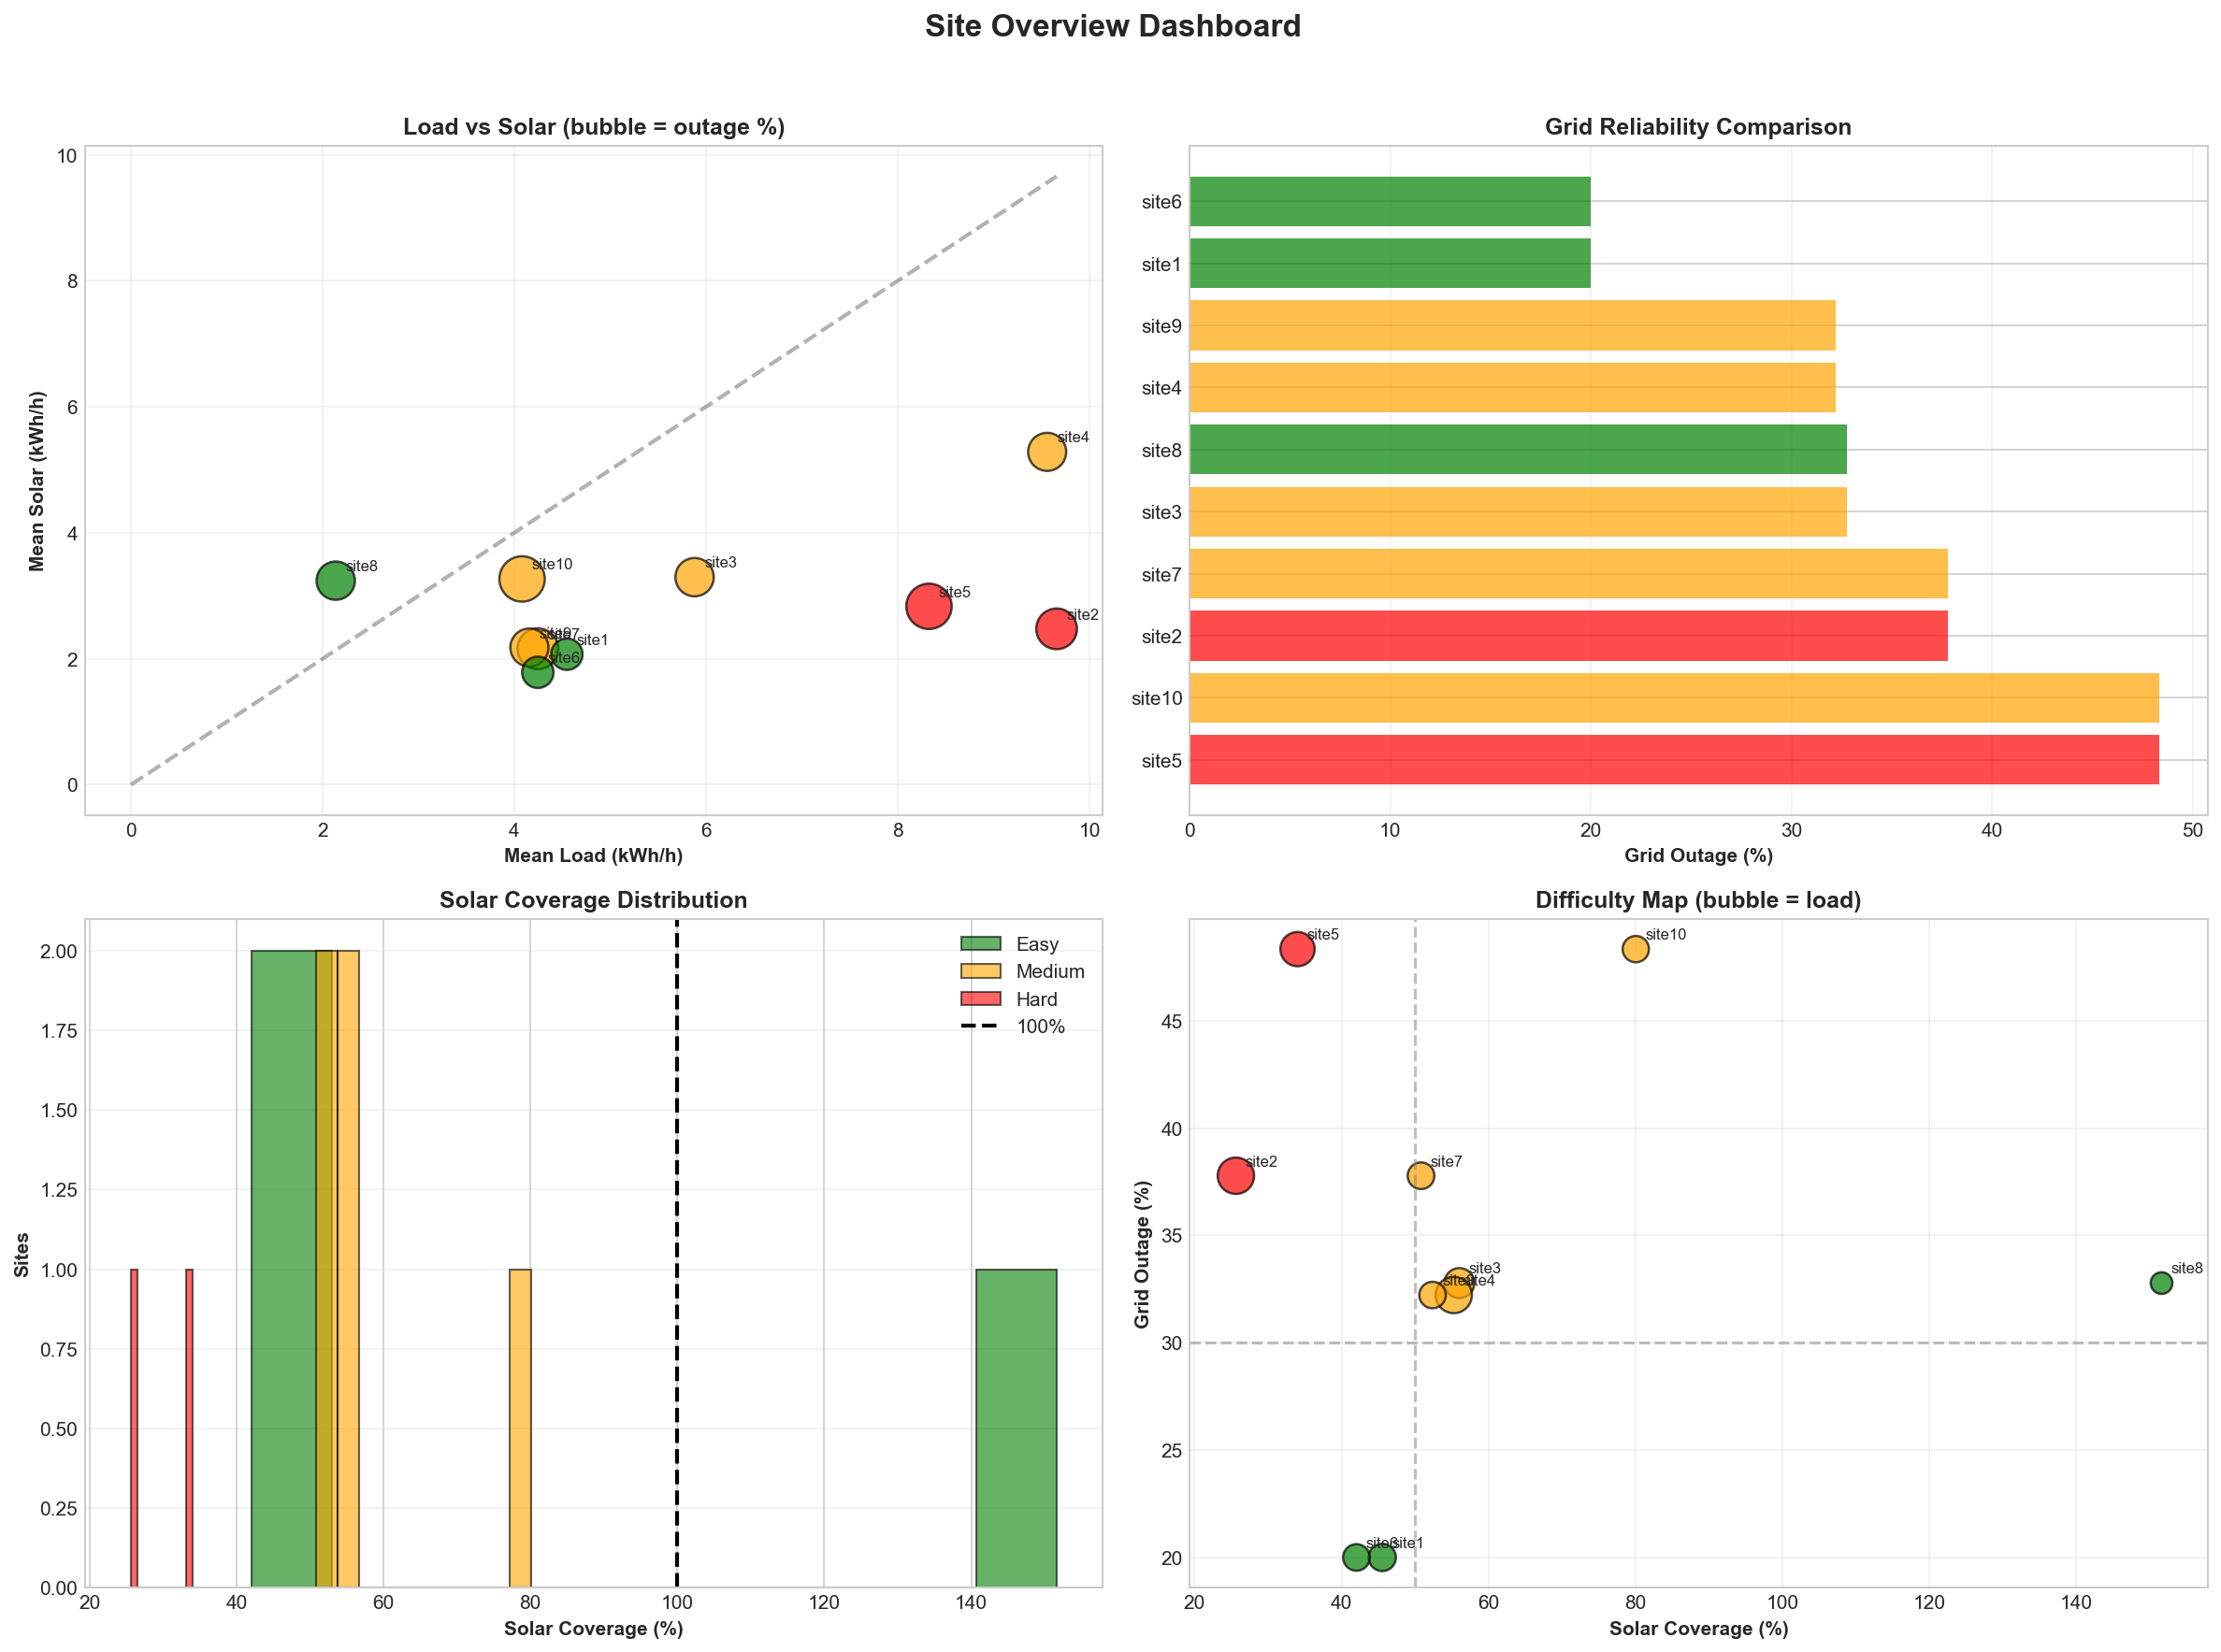
\includegraphics[width=\textwidth, clip=true]{images/fig1_site_overview}
\caption{Site overview dashboard for all ten ITU/Zindi sites.
\textit{Top-left:} mean load vs.\ mean solar scatter; bubble size encodes
outage rate.  Sites above the diagonal are solar-surplus; sites below are
solar-deficit.  \textit{Top-right:} grid outage rate per site, sorted by
severity; sites~5 and~10 have the highest outage exposure ($\approx$48\%).
\textit{Bottom-left:} distribution of solar coverage levels; one site
(site~8) exceeds 100\%.  \textit{Bottom-right:} difficulty map — solar
coverage vs.\ grid outage rate with bubble size proportional to load;
Hard sites (red) occupy the high-outage, low-solar quadrant.}
\label{fig:site_characteristics}
\end{figure}

Three observations emerge from the site statistics.

\textbf{High-load, low-solar, weak-grid sites are the most difficult.}
Sites~2 and~5 combine high average demand (9.66 and 8.32\,kWh/h), poor
solar coverage (25.6\% and 34.0\%), and frequent grid outages (62.2\% and
51.7\% availability).  These sites create persistent energy deficits during
grid loss and place the greatest pressure on diesel backup and fuel inventory
management.

\textbf{Site~8 is solar-surplus.}
With solar coverage of 151.6\%, site~8 generates more PV energy than it
consumes on average.  DG activation is rare; reliability is rarely
threatened.  This site establishes a natural performance ceiling against
which other sites can be compared.

\textbf{Battery capacity is not uniformly matched to load.}
Despite having the highest outage frequency in the dataset, site~5 has only
20.5\,kWh of battery storage --- less than high-load sites~2, 3, and~4 which
carry 41\,kWh banks.  On site~5, diesel inventory is therefore a primary
reliability lever even after battery dispatch is optimised.


% ============================================================
\section{Diurnal Load and Solar Patterns}
\label{sec:diurnal_patterns}
% ============================================================

In addition to cross-site variability, the dataset exhibits a clear and
structured diurnal pattern.  Figure~\ref{fig:diurnal_profiles} shows the mean
hourly load demand and mean hourly solar generation averaged across all sites.

\begin{figure}[htbp]
\centering
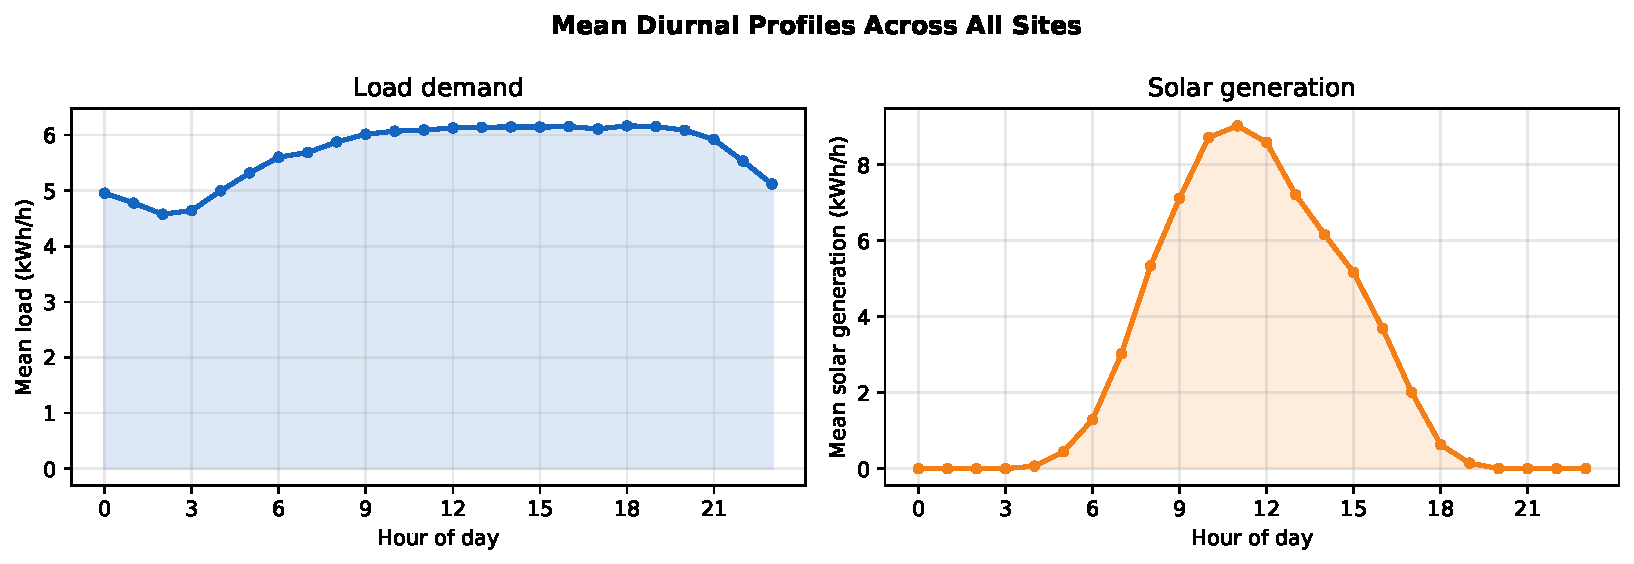
\includegraphics[width=\textwidth, clip=true]{images/fig_diurnal_profiles}
\caption{Mean diurnal load and solar profiles averaged across all ten sites.
Load is elevated from 08:00--20:00, peaking near 6.2\,kWh/h in the
mid-afternoon.  Solar generation peaks near 11:00 at 9.0\,kWh/h before
declining through the afternoon.  The temporal mismatch between peak solar
(11:00) and peak load (14:00--18:00) creates a recurring afternoon deficit
window that battery, grid, or DG must cover.}
\label{fig:diurnal_profiles}
\end{figure}

Two observations are relevant to the control problem.  First, solar generation
is effectively zero from 20:00 to 05:00; all overnight demand must be met by
stored energy, grid supply, or DG operation.  Second, although mean daytime
solar output is substantial, it does not perfectly align with demand: the
solar peak precedes the load peak by several hours.  This creates predictable
deficit windows before sunrise and in the late afternoon, reinforcing the need
for sequential energy management rather than purely myopic dispatch.


% ============================================================
\section{Grid Outage Structure}
\label{sec:grid_patterns}
% ============================================================
\begin{sloppypar}
Grid availability is a defining feature of the dataset because it is the
primary exogenous disturbance that forces switching between renewables,
battery, and diesel-backed operation.  Figure~\ref{fig:grid_raster} shows the
hour-by-hour outage raster for all ten sites over the full 60-day window.
\end{sloppypar}

\begin{figure}[htbp]
\centering
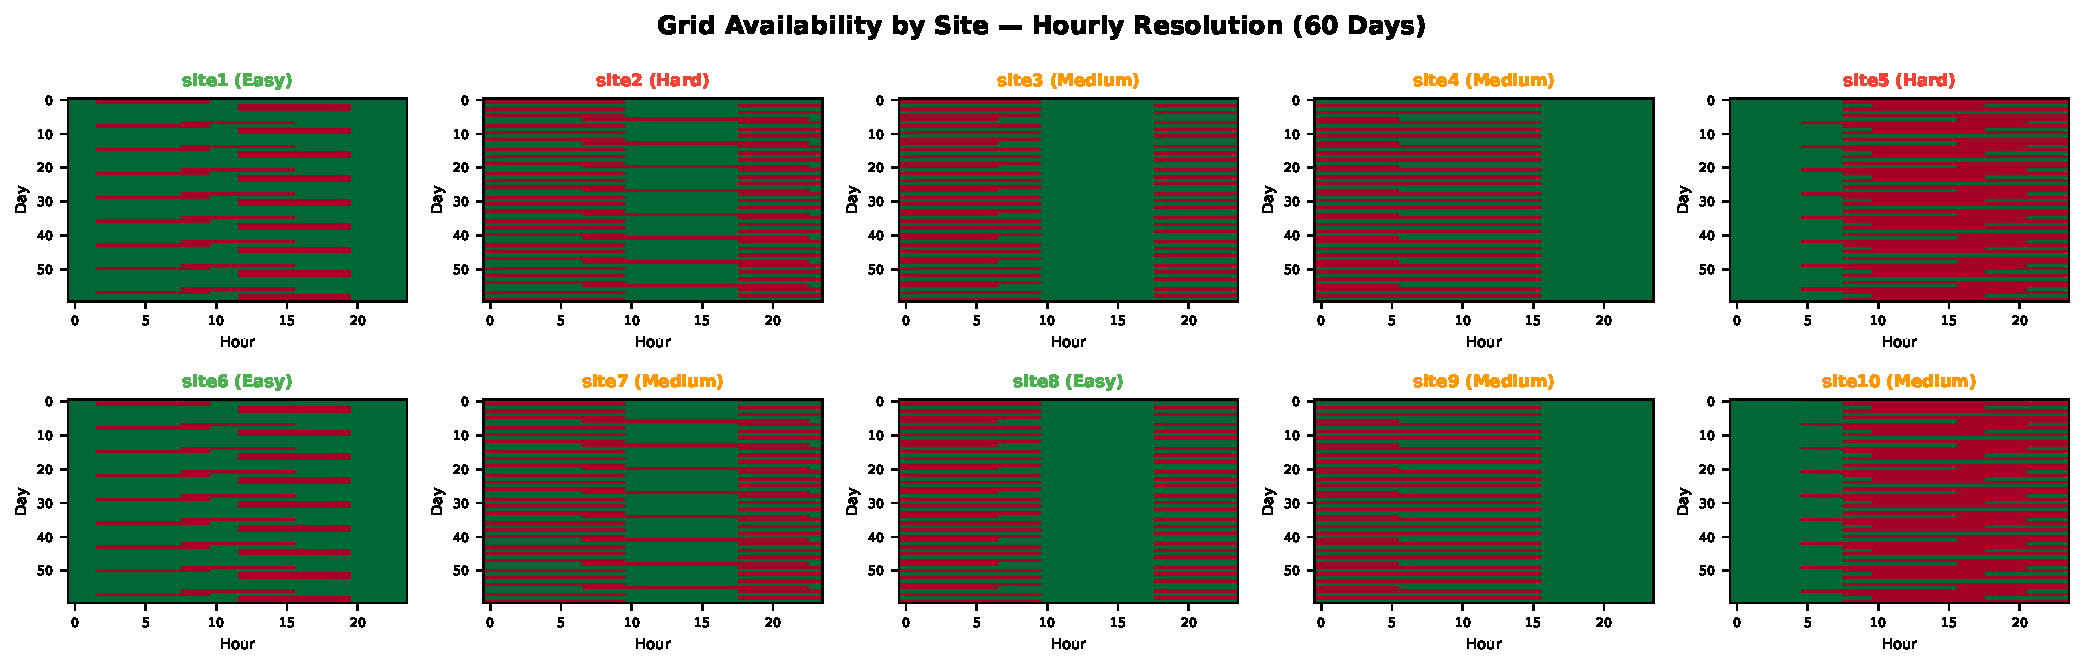
\includegraphics[width=\textwidth, clip=true]{images/fig_grid_raster}
\caption{Grid availability raster: each row is one day, each column one hour
of day.  Green = grid available; red = outage.  Sites~1 and~6 show short,
structured nocturnal outages (8\,h blocks).  Sites~2, 5, 7, and~10 exhibit
extended daily outage patterns (up to 16\,h).  The block structure indicates
that outages are not purely random but follow a predictable daily schedule,
a regularity that a non-myopic RL policy can exploit.}
\label{fig:grid_raster}
\end{figure}

Table~\ref{tab:outage_stats} quantifies outage structure per site.  The
maximum observed outage duration is 16\,h across all sites.  This exceeds the
24-h mean lead time of the normal logistics scenario, confirming that a single
extended outage can deplete a partially-stocked tank before a delivery
arrives --- the core failure mode the inventory-aware policy must prevent.

\begin{table}[htb]
\centering
\small
\caption{Grid outage statistics per site.}
\label{tab:outage_stats}
\begin{tabular}{lrrrl}
\toprule
\textbf{Site} & \textbf{Outage events} & \textbf{Mean duration (h)} &
\textbf{Max duration (h)} & \textbf{Class} \\
\midrule
site1  & 36 &  8.0 &  8 & Easy   \\
site2  & 34 & 16.0 & 16 & Hard   \\
site3  & 34 & 13.9 & 16 & Medium \\
site4  & 34 & 13.6 & 16 & Medium \\
site5  & 52 & 13.4 & 16 & Hard   \\
site6  & 36 &  8.0 &  8 & Easy   \\
site7  & 34 & 16.0 & 16 & Medium \\
site8  & 34 & 13.9 & 16 & Easy   \\
site9  & 34 & 13.6 & 16 & Medium \\
site10 & 52 & 13.4 & 16 & Medium \\
\bottomrule
\end{tabular}
\end{table}

Site~5 stands out with 52 outage events --- the highest frequency in the
dataset --- combined with the lowest solar coverage and a small battery.
This triple constraint makes it the most demanding test for any inventory or
dispatch policy, and it is expected to be among the most informative sites
in the experimental evaluation.


% ============================================================
\section{Scarcity and Surplus Regimes}
\label{sec:scarcity_surplus}
% ============================================================

Exploratory analysis reveals that the dataset naturally separates into two
operational regimes.

\textbf{Scarcity regime.}
In several sites, mean deficit during outage is high and battery autonomy is
insufficient to cover the longest observed outage block.  In such settings,
diesel is not a marginal backup but a critical reliability resource.  A
controller that ignores fuel inventory in these sites risks stockout during
repeated weak-grid periods.  Figure~\ref{fig:rl_stress} quantifies this
across four dimensions: battery autonomy relative to grid outage frequency,
battery sizing against worst-case outage duration, 95th-percentile deficit
severity during outages, and the fraction of solar-surplus hours per site.

\begin{figure}[htbp]
\centering
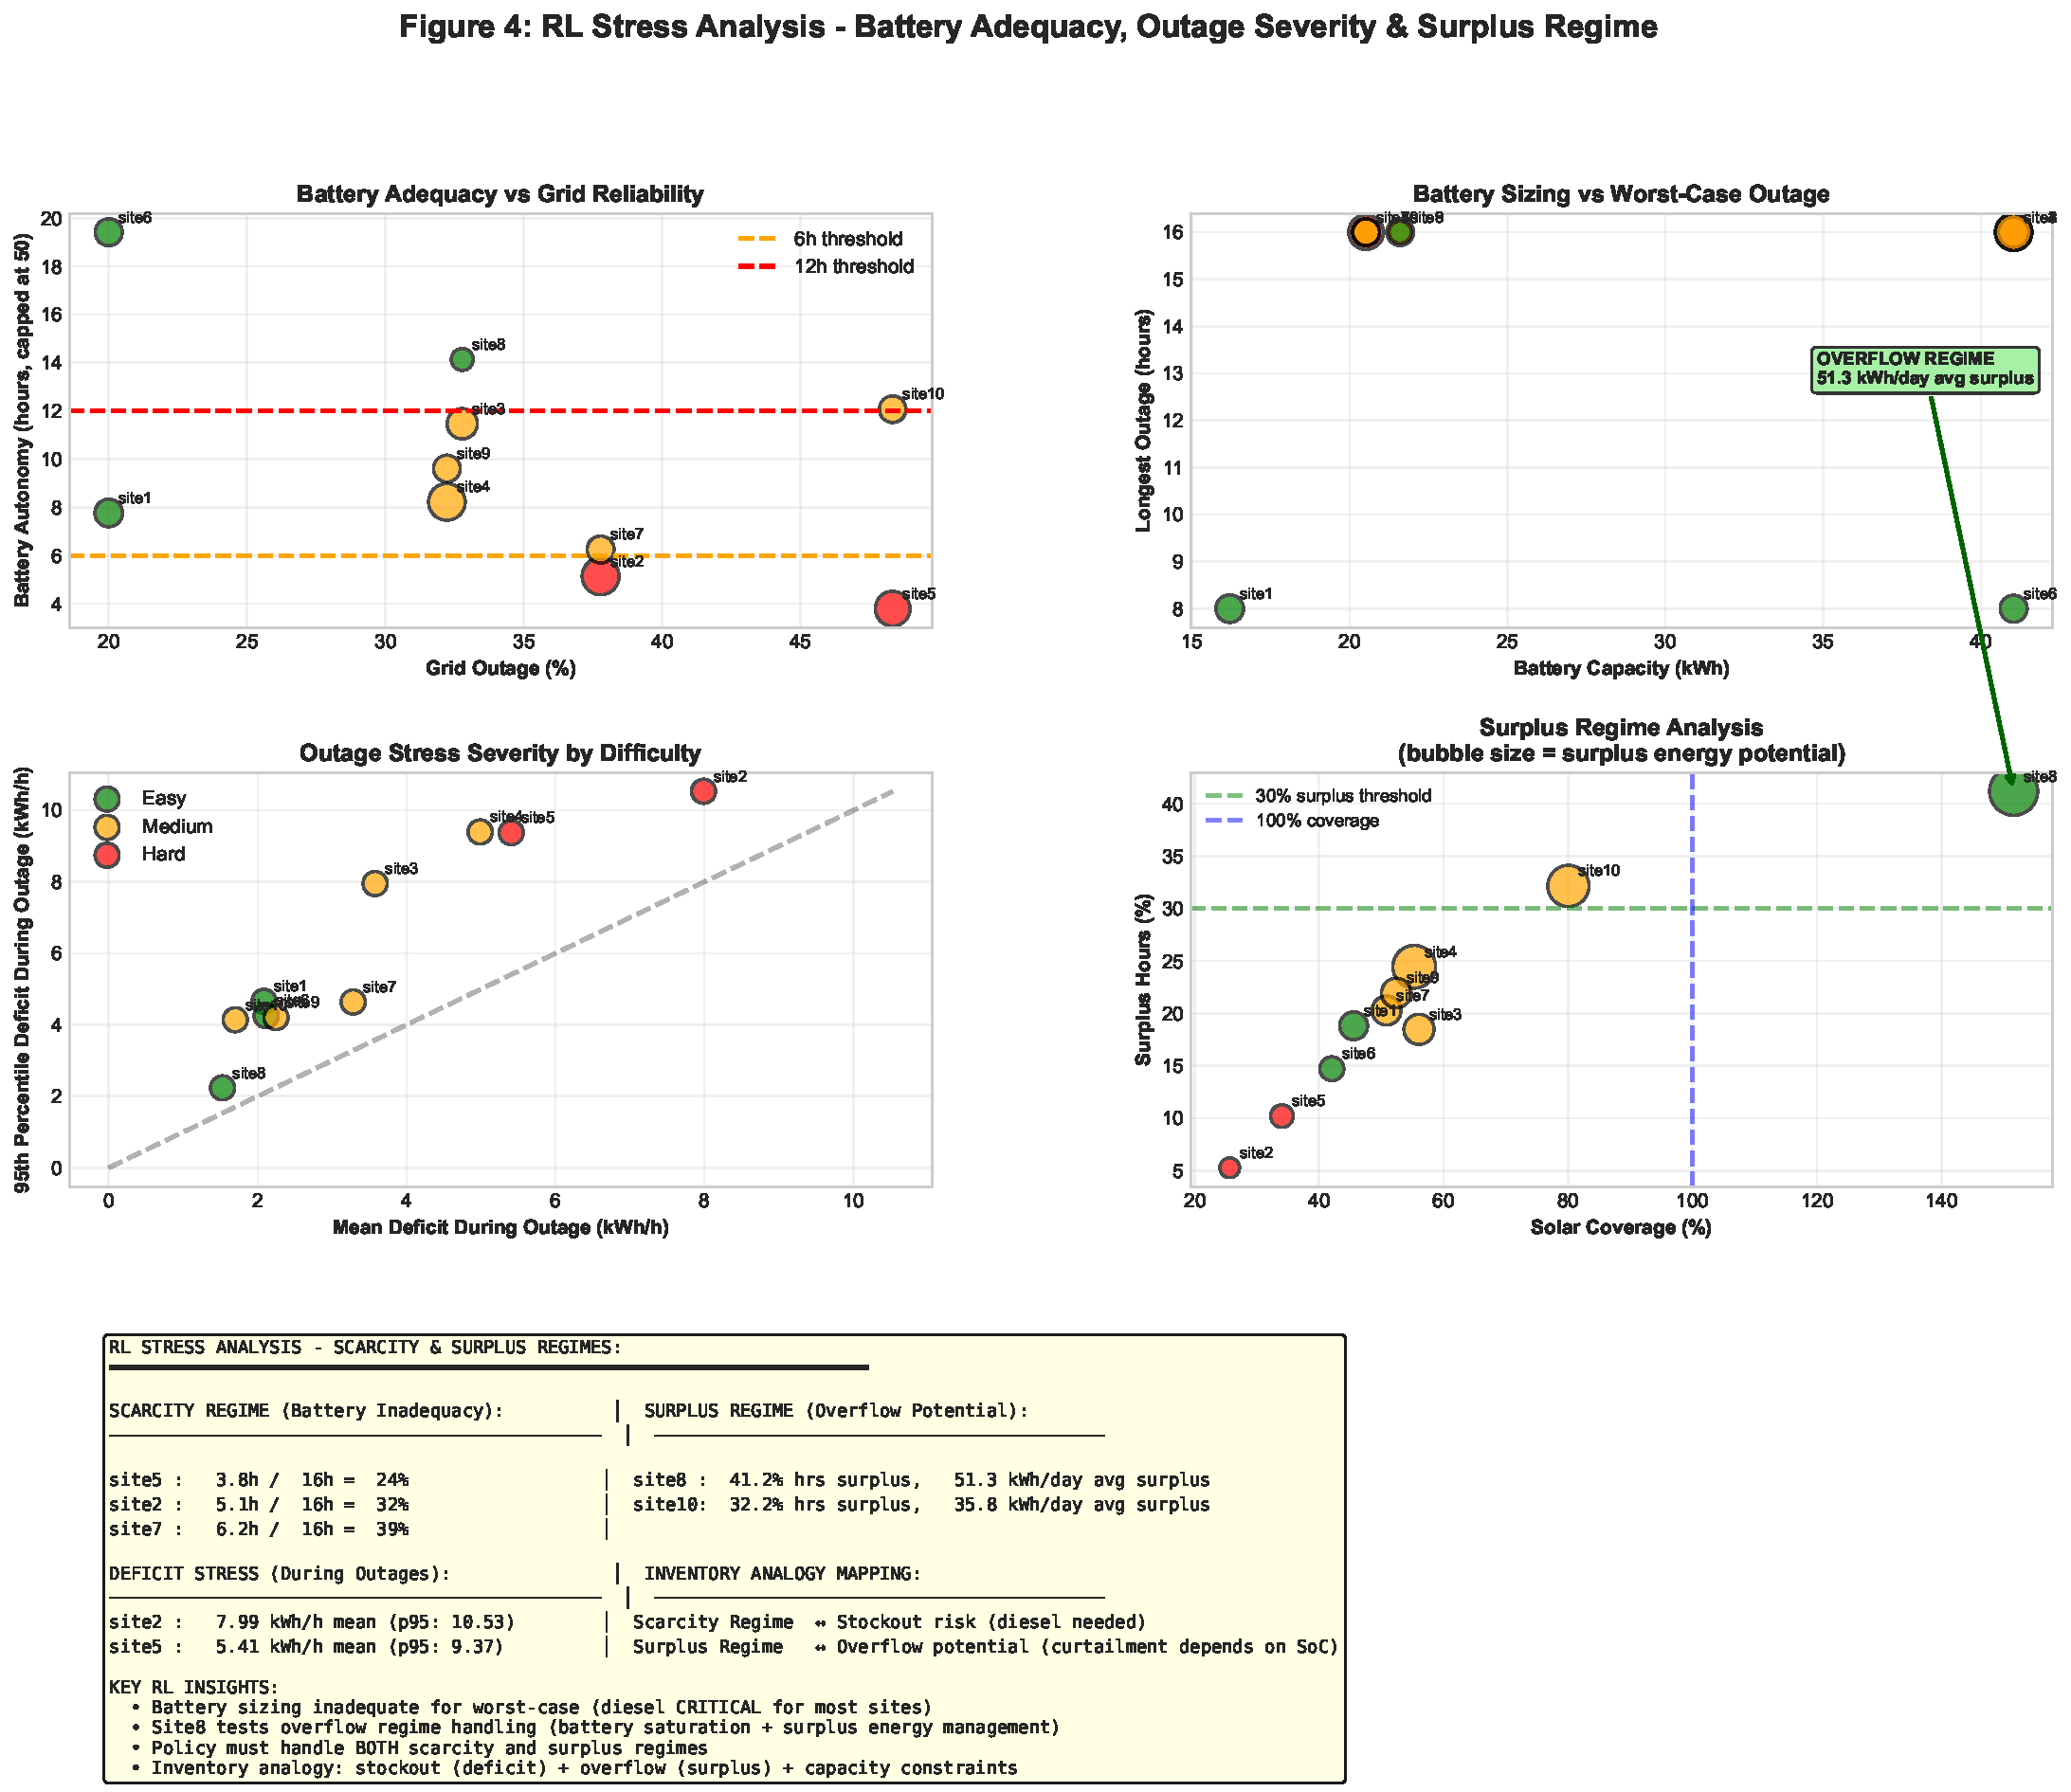
\includegraphics[width=\textwidth, clip=true]{images/fig4_rl_stress_analysis}
\caption{RL stress analysis across all ten sites.
\textit{Top-left:} battery autonomy (hours) vs.\ grid outage rate; sites
below the 6\,h threshold (orange dashed) cannot bridge a typical outage on
battery alone.  Sites~2 and~5 fall well below this line.
\textit{Top-right:} battery capacity vs.\ longest observed outage; most sites
face worst-case outages of 16\,h with batteries sized for far less.
\textit{Bottom-left:} mean vs.\ 95th-percentile deficit during outages;
sites~2 and~5 (red) show the highest deficit stress.
\textit{Bottom-right:} surplus hours vs.\ solar coverage; site~8 is in the
overflow regime with 41\% surplus hours and 51\,kWh/day average surplus.
The summary panel confirms the scarcity--surplus split: sites~2 and~5 are
battery-inadequate (inventory-critical), while site~8 and partially site~10
face overflow potential.}
\label{fig:rl_stress}
\end{figure}

Figure~\ref{fig:net_load_cdf} shows the net load
CDF for all sites; the Hard sites (site~2 and site~5, red) have right-shifted
distributions, confirming sustained positive net load and high reliance on
supplementary energy sources.

\textbf{Surplus regime.}
At the other extreme, site~8 is clearly solar-surplus, with solar coverage
of 151.6\% and net load negative for 41\% of hours (average surplus
51\,kWh/day).  Solar generation peaks at 10.5\,kWh/h near 10:00 while
load holds steady near 2\,kWh/h, saturating the 21.6\,kWh battery on
most days.  Here the main challenge is not avoiding shortage but handling
battery saturation and curtailment.  Site~8 behaves qualitatively
differently from the scarcity-dominated sites; its detailed profile is
in Appendix~\ref{app:site_profiles}.

\begin{figure}[htbp]
\centering
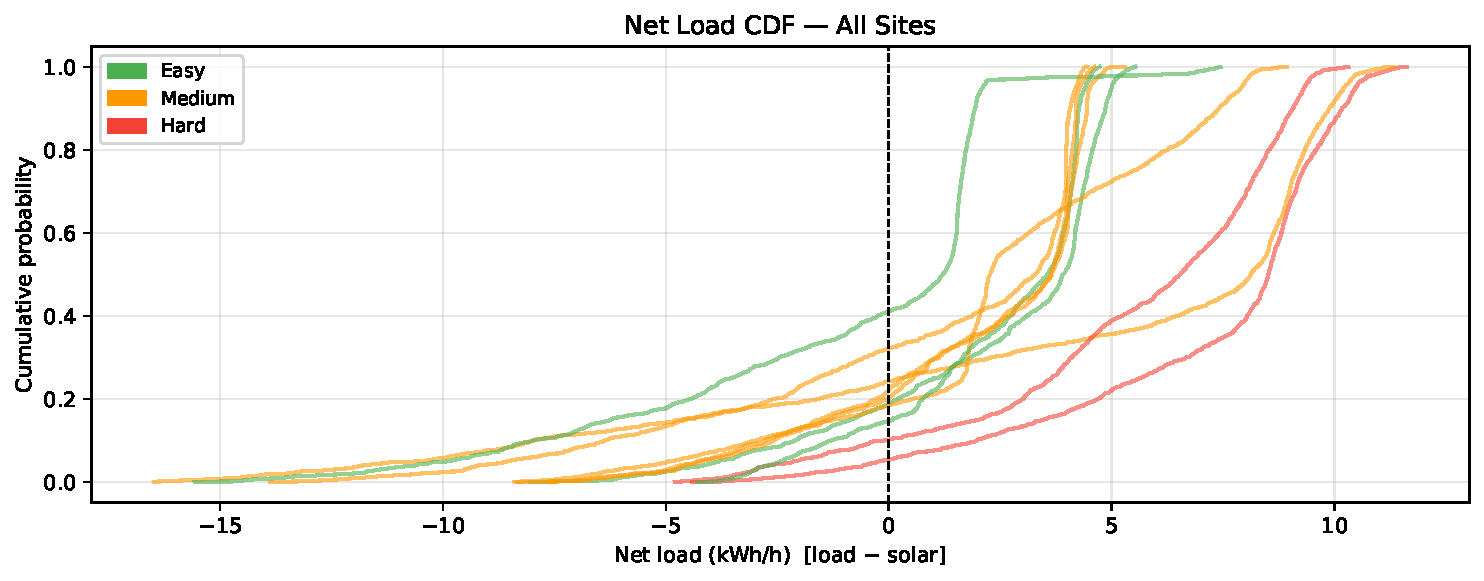
\includegraphics[width=0.85\textwidth, clip=true]{images/fig_net_load_cdf}
\caption{Cumulative distribution of net load across all sites.  The dashed
vertical line at zero separates solar-deficit hours (right) from solar-surplus
hours (left).  Hard sites (red) are entirely in deficit; site~8 (green) crosses
zero near $p = 0.6$, confirming majority solar surplus.}
\label{fig:net_load_cdf}
\end{figure}

This regime split is important for the experimental design.  Easy and
surplus-regime sites are useful robustness checks but offer limited
discriminatory power where operating conditions are mild.
The scarcity-regime sites --- primarily site~2, site~5, and site~10 under
adverse logistics conditions --- are structurally where inventory-aware
control is most likely to reveal a measurable advantage.

The main policy comparison uses all ten sites,
while selected sensitivity and extended algorithm
comparisons use smaller, explicitly identified
subsets for focused analysis.

\begin{quote}
\textbf{Note on site terminology used elsewhere in this thesis.} This
scarcity-regime grouping (site~2, site~5, site~10) and the Hard/Medium/Easy
difficulty classification of Section~\ref{sec:site_classification} below
are both derived from the EDA in this chapter. A separate, differently
selected three-site subset (site~2, site~5, site~7) is used in
Chapter~\ref{chap:results} for finer-grained sensitivity analyses; that
subset was chosen to provide diverse operating characteristics (load,
solar generation and outage behaviour) for the detailed sensitivity
analyses, rather than to represent the scarcity-based difficulty ranking
introduced in this chapter. The scarcity-regime classification introduced here is therefore used for
exploratory data analysis, whereas the site~2/site~5/site~7 subset is
used only for the detailed sensitivity analyses described in
Chapter~\ref{chap:results}.
\end{quote}

This chapter characterises the dataset, establishes its operational
properties through exploratory data analysis, and motivates the
representative site selection used throughout the thesis. The complete experimental protocol and evaluation methodology are
presented in Chapters~\ref{chap:methodology}
and~\ref{chap:results}.

These observations motivate the representative site selection adopted in
this chapter and provide the empirical basis for the experimental
evaluation protocol introduced in
Chapter~\ref{chap:methodology}.

% ============================================================
\section{Representative Site Profile}
\label{sec:site_profiles}
% ============================================================

To make the stress analysis concrete, Figure~\ref{fig:site5_analysis}
presents the enhanced profile for site~5 --- the most operationally
demanding site in the dataset and the primary test case for
inventory-aware control.  Profiles for all ten sites are provided in
Appendix~\ref{app:site_profiles}.

Site~5 combines high outage frequency (52 events over 60 days, the
highest in the dataset), low solar coverage (34\%), and a small battery
(20.5\,kWh, autonomy 3.8\,h).  The battery covers only 24\% of the
longest observed 16-hour outage.  Four outage events exceed the 12-hour
threshold.  Outage-conditioned mean deficit is 5.41\,kWh/h (95th
percentile 9.37\,kWh/h).  Under these conditions any policy that
underestimates diesel consumption risk faces repeated unserved load
events.
 This site therefore provides one of the most discriminating test
cases for comparing inventory-aware and inventory-blind control.

\begin{figure}[htbp]
\centering
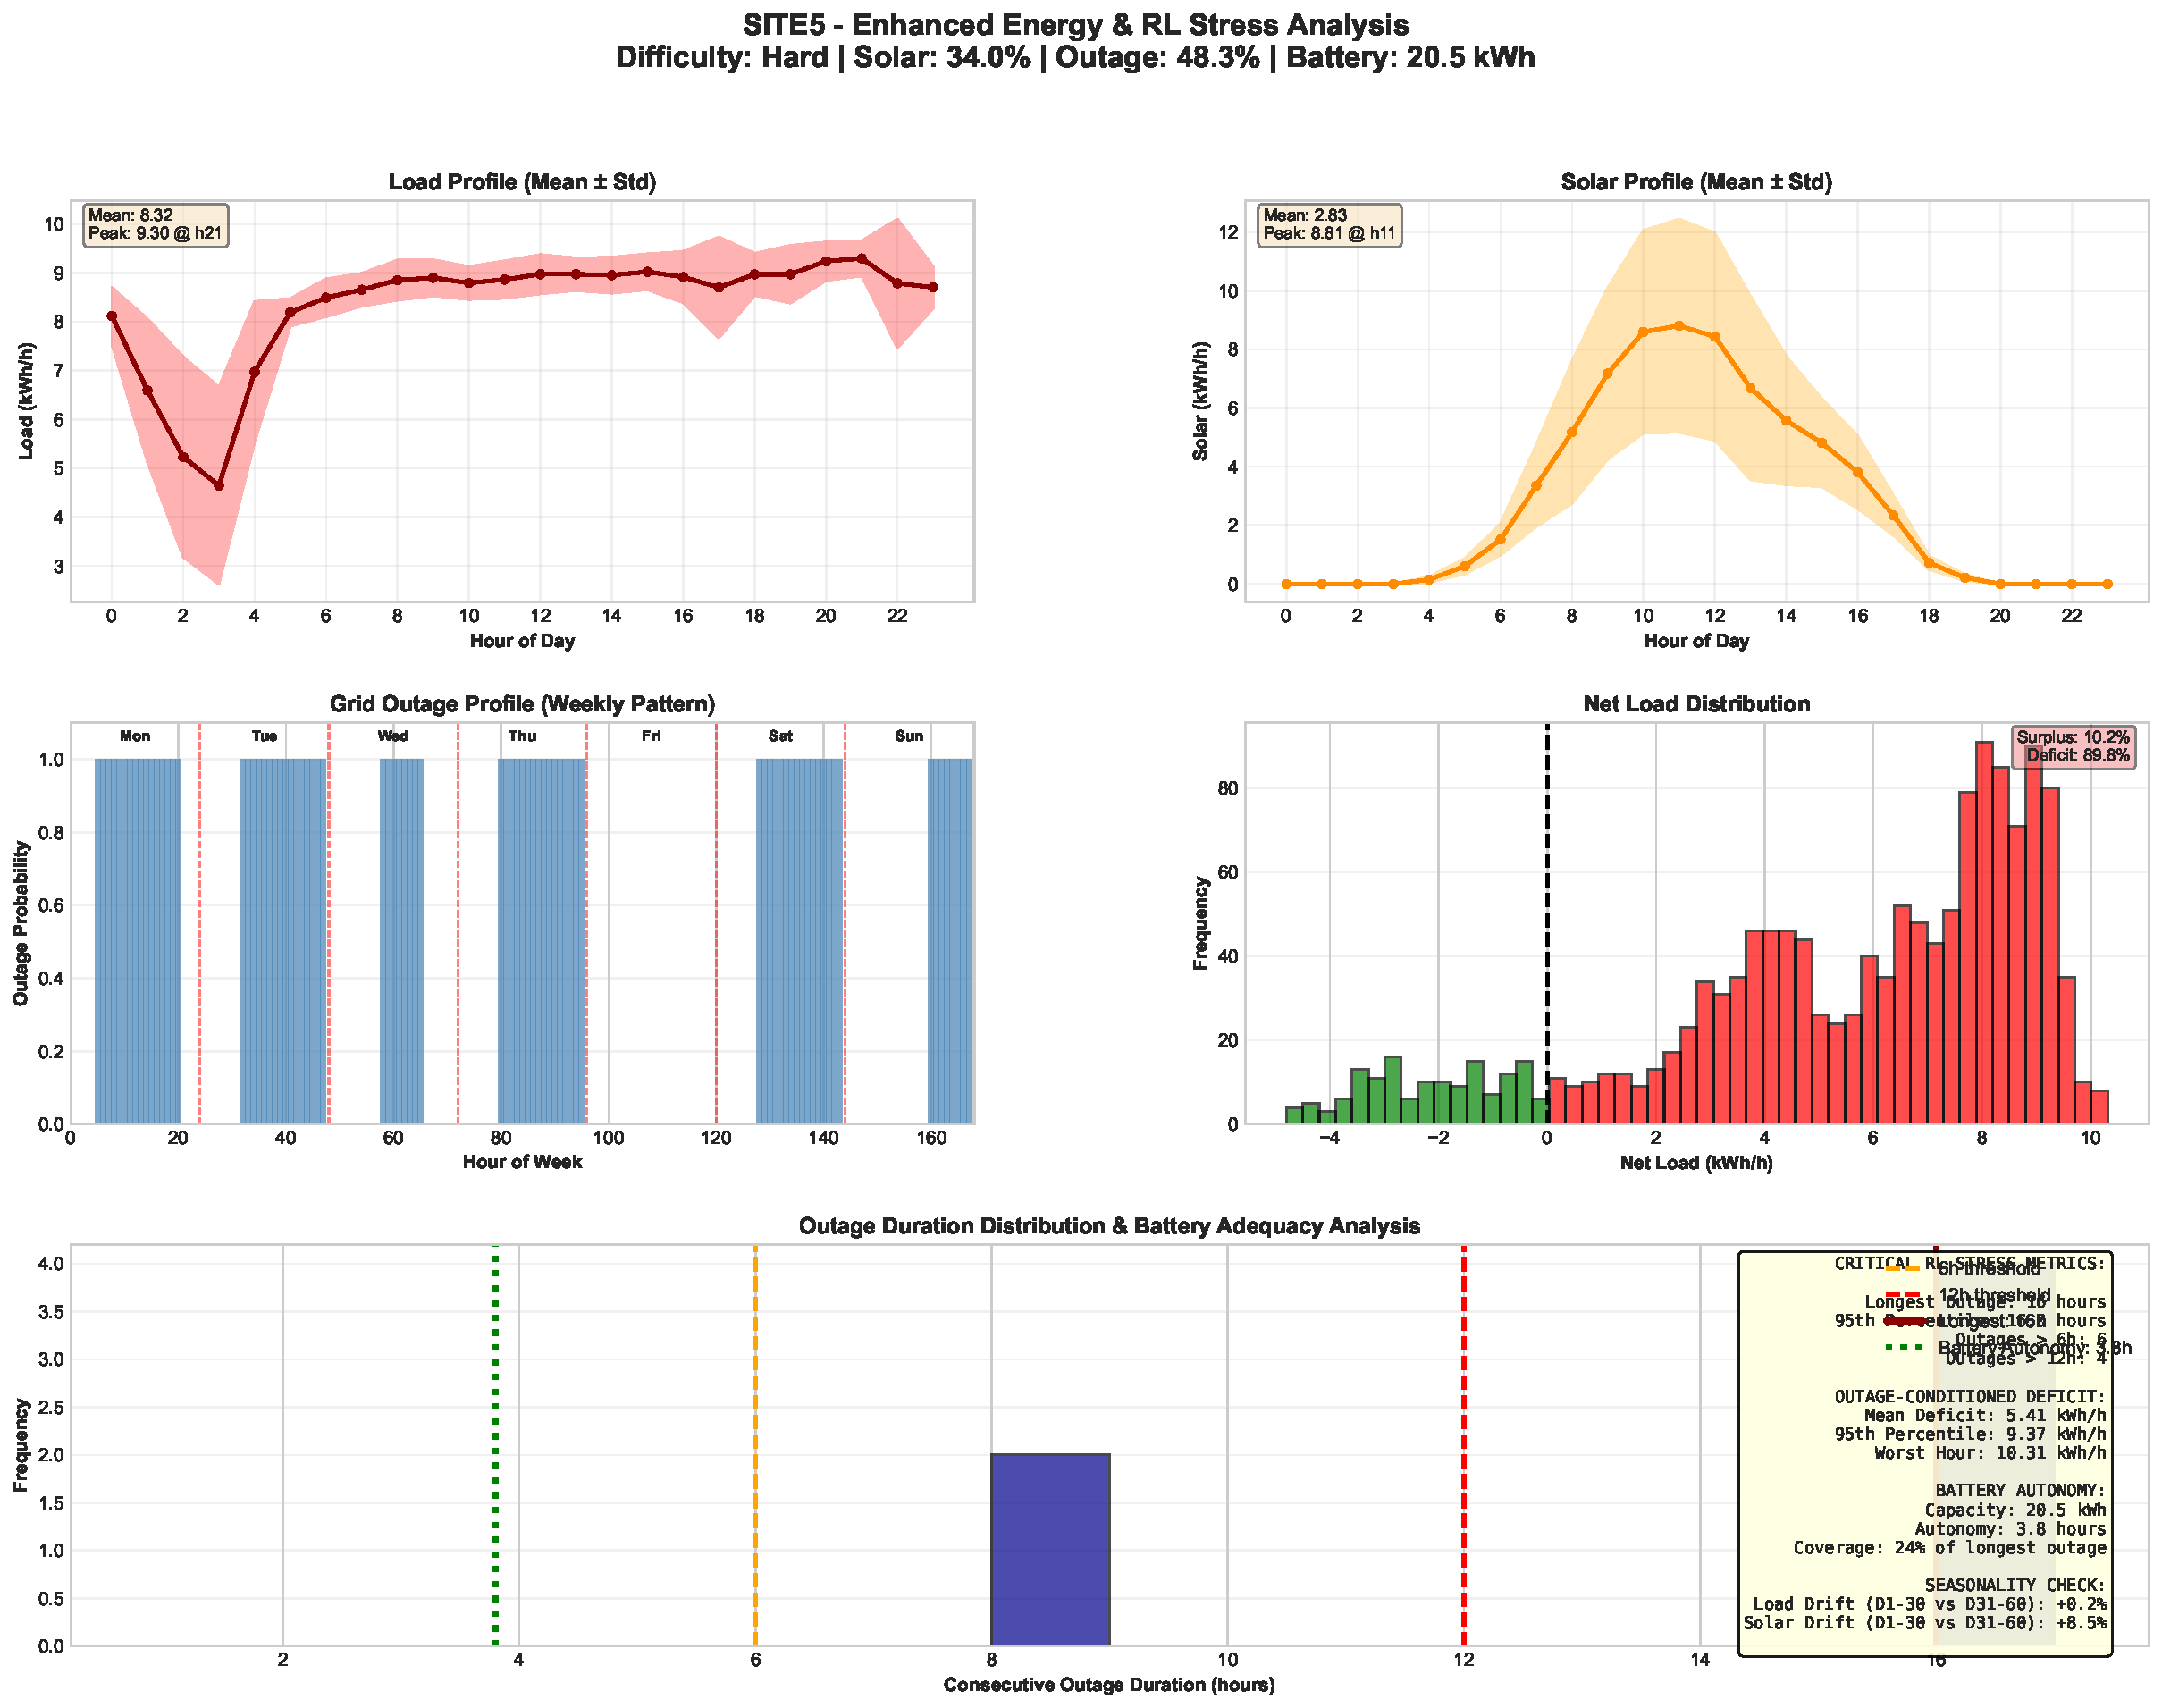
\includegraphics[width=\textwidth, clip=true]{images/site5_enhanced_analysis}
\caption{Enhanced stress analysis for site~5 (Hard).
Battery autonomy of 3.8\,h covers only 24\% of the longest outage.
52 outage events over 60 days --- the highest frequency in the dataset.
Four events exceed the 12-hour threshold (red dashed line).
Outage-conditioned 95th-percentile deficit is 9.37\,kWh/h.}
\label{fig:site5_analysis}
\end{figure}


% ============================================================
\section{Site Difficulty Classification}
\label{sec:site_classification}
% ============================================================

To organise the experiments, sites are grouped into difficulty classes using a
composite score combining grid outage frequency, solar coverage, and mean net
load.  Sites scoring 4 are classified Hard; 2 Medium; 1 Easy.
Table~\ref{tab:difficulty} shows the classification.

\begin{table}[htb]
\centering
\small
\caption{Site difficulty classification and primary challenge.  Constrained
sites (frequent outages, low solar, inadequate battery autonomy) receive
focused statistical analysis in Chapter~\ref{chap:results}.}
\label{tab:difficulty}
\begin{tabular}{p{3.8cm}p{1.5cm}p{1.5cm}p{5.0cm}}
\toprule
\textbf{Site(s)} & \textbf{Class} & \textbf{Outage (\%)} & \textbf{Primary challenge} \\
\midrule
site2, site5                       & Hard   & 38--48 & High load, low solar, frequent outages;
                                                        battery autonomy inadequate for longest outages \\
site3, site4, site7, site9, site10 & Medium & 33--48 & Moderate load-solar balance; grid
                                                        reliability moderate \\
site1, site6, site8                & Easy   & 20--33 & Adequate solar or high grid availability;
                                                        outage stress low \\
\bottomrule
\end{tabular}
\end{table}

\begin{quote}
\textbf{Note on site~10.}
Site~10 is classified Medium by composite score (solar coverage 80\%, but
outage frequency 51.7\%).  Its battery autonomy of 12.1\,h covers only
75\% of the longest observed 16-hour outage, and four outage events exceed
the 12-hour threshold.  Under adverse logistics conditions, site~10 is
structurally exposed to the same reliability risks as the Hard sites.
Results tables note this distinction where relevant.
\end{quote}

The classification is a practical organising tool, not a research outcome.
It separates sites where operating stress is structurally high
from those where conditions are comparatively mild.


% ============================================================
\section{Dataset Limitations}
\label{sec:dataset_limitations}
% ============================================================

The dataset is well suited to the present study, but three limitations must
be stated clearly.

\textbf{No diesel logistics records.}
The dataset provides load, solar, grid availability, and battery capacity, but
not diesel delivery events, lead times, or fuel replenishment logs.  The
delivery-pipeline component of the simulator is therefore synthetic.  This
is the sole component of the simulation not grounded in the ITU data, and
is clearly documented as such in Chapter~\ref{chap:methodology}.

\textbf{Limited time horizon.}
Each site contains 60 days of observations, covering a single operating
season.  Solar generation patterns and outage frequencies may differ in other
seasons; results should be interpreted as representative of the recorded
conditions rather than year-round operation.

\textbf{Assumed tank capacity.}
Absolute diesel tank capacity is not provided.  The assumption
$C^{\Tank} = 72\bar{D}$ gives physically plausible values (approximately
three days of full-load backup across all sites), but real tank sizes may
differ.  Sensitivity to this assumption is partially captured by randomising
initial inventory over $[0.3,\,0.9]\,C^{\Tank}$ during evaluation.


% ============================================================
\section{Chapter Summary}
\label{sec:dataset_summary}
% ============================================================

This chapter established the empirical foundation of the study.  The
ITU/Zindi dataset provides ten heterogeneous tower sites with hourly load,
solar, and grid traces that are replayed directly in the simulator.
Preprocessing produces clean site-level time series with consistent indexing,
derived net load, and a principled train/test split.  Exploratory analysis
shows that the sites span both scarcity-dominated and surplus-dominated
regimes, with large differences in outage severity, battery adequacy, and
renewable coverage.  These characteristics justify the multi-site evaluation
design used in the remainder of the thesis and explain why inventory-aware
control is most likely to show a measurable advantage in the most constrained
sites.
    \chapter{Experimental Execution and Implementation}
\label{chap:experimental-execution}
\setlength{\emergencystretch}{1.5em}

Chapter~\ref{chap:methodology} defined the experimental design: the
simulator architecture, policy set, and evaluation protocol. This
chapter records how that design was executed: the implementation
sequence, the training workload actually run, how the ablation set
evolved during development, and the statistical framework used for the
confirmatory evaluation. The exploratory experiments described here
informed the final experimental design but are not included in the
confirmatory hypothesis-testing results reported in
Chapter~\ref{chap:results}.
% ============================================================
\section{Implementation Sequence}
\label{sec:impl_overview}
% ============================================================

The implementation was built in layers, each producing runnable,
testable output before the next began, so that no layer depended on
untested components from a lower one (Figure~\ref{fig:exec_pipeline},
Table~\ref{tab:impl_sequence}).

\begin{figure}[htbp]
\centering
\resizebox{\textwidth}{!}{%
\begin{tikzpicture}[
  node distance=0.5cm and 1.3cm,
  box/.style={draw, rounded corners, align=center,
              minimum width=2.6cm, minimum height=0.8cm, font=\footnotesize}
]
\node[box] (data)     {Data pipeline};
\node[box, right=of data]     (sim)   {Simulator};
\node[box, right=of sim]      (base)  {Baselines};
\node[box, right=of base]     (rl)    {RL agent};
\node[box, below=1.0cm of data] (trackb) {TrackB};
\node[box, right=of trackb]   (abl)   {Ablations};
\node[box, right=of abl]      (opt)   {Optimisation baselines};
\node[box, right=of opt]      (eval)  {Full evaluation (44{,}000 rollouts)};

\draw[->] (data) -- (sim);
\draw[->] (sim)  -- (base);
\draw[->] (base) -- (rl);
\draw[->] (rl.south) -- ++(0,-0.3) -| (trackb.north);
\draw[->] (trackb) -- (abl);
\draw[->] (abl)  -- (opt);
\draw[->] (opt)  -- (eval);
\end{tikzpicture}%
}
\caption{Experiment execution pipeline, following the layer order of
Table~\ref{tab:impl_sequence}.}
\label{fig:exec_pipeline}
\end{figure}

\begin{table}[htb]
\centering
\small
\caption{Implementation execution sequence.}
\label{tab:impl_sequence}
\begin{tabular}{cp{2.6cm}p{8.2cm}}
\toprule
\textbf{Layer} & \textbf{Component} & \textbf{Deliverable} \\
\midrule
1 & Data pipeline   & ITU/Zindi site CSVs loaded, validated, split \\
2 & Simulator       & \texttt{TelecomEnv} passing unit tests on all transitions \\
3 & Baselines       & B0, B1 rule-based policies producing first cost numbers \\
4 & RL agent        & RLInv training on a single site, converging \\
5 & TrackB          & Decomposed $(s,S)$ + PPO dispatch training \\
6 & Ablations       & A5, A6, A7 variants trained and evaluated \\
7 & Optimisation baselines & MPC and Oracle-MPC MILP dispatch (HiGHS solver) \\
8 & Full evaluation & 44{,}000-rollout campaign complete (36{,}000 core $+$
                        8{,}000 exploratory) \\
\bottomrule
\end{tabular}
\end{table}

The repository structure follows this layer ordering
(\texttt{env/}, \texttt{baselines/}, \texttt{train/}, \texttt{eval/}),
with all hyperparameters centralised in a single
\texttt{config/hparams.yaml} and no magic numbers in training scripts.

Several implementation decisions made during this build are documented
in Chapter~\ref{chap:methodology}'s Implementation Deviations table
rather than repeated here, to avoid duplicating that content; this
chapter records only decisions specific to \emph{how} the build was
carried out, not \emph{what} was built.

\begin{sloppypar}
\paragraph{Parallel environment count.} The training configuration
targeted eight parallel \texttt{SubprocVecEnv} workers. On the
development machine, an OS limit on process handles caused intermittent
failures at eight workers, so the count was reduced to four for all
training runs. This roughly doubles wall-clock time per run but does not
affect the PPO gradient estimate's statistical properties, since the
effective batch size is preserved by scaling $n_{\text{steps}}$
proportionally.
\end{sloppypar}

\paragraph{Observation normalisation synchronisation.} An early
implementation issue caused anomalously high variance across seeds
during evaluation, traced to \texttt{VecNormalize} statistics not being
frozen and synchronised between training and evaluation environments. A
custom evaluation callback was added to copy the training
\texttt{VecNormalize} state to the evaluation environment before each
validation pass; the anomalous variance disappeared once this was
corrected.


% ============================================================
\section{Training Workload}
\label{sec:training_execution}
% ============================================================

Table~\ref{tab:training_workload} summarises the training workload
actually executed for the final Phase 3 campaign.

\begin{table}[htb]
\centering
\small
\setlength{\tabcolsep}{5pt}
\caption{Total training workload, final campaign.}
\label{tab:training_workload}
\begin{tabular}{lrp{5.8cm}}
\toprule
\textbf{Item} & \textbf{Count} & \textbf{Note} \\
\midrule
Sites                    & 10  & All ITU/Zindi sites \\
Seeds per policy         & 10  & 42, 123, 777, 7, 13, 21, 99, 314, 500, 999 \\
RL policies trained      & 5   & RLInv, TrackB, A5, A6, A7 (standard PPO,
                                 no masking) \\
Non-RL policies          & 4   & B0, B1 (rule-based); MPC, Oracle-MPC
                                 (optimisation-based) --- no training \\
Timesteps per RL run     & 400{,}000 & Per site per seed \\
Total RL training runs   & 500 & 5 trained policies $\times$ 10 sites
                                 $\times$ 10 seeds \\
Training budget          & Fixed & 400{,}000 steps, used consistently across all runs \\
\bottomrule
\end{tabular}
\end{table}

\subsection{Training Convergence Assessment}

A convergence check on three representative sites (1, 5, and 7) found no
consistent benefit from extending training beyond 400{,}000 steps.
The 400{,}000-step checkpoint was retained for all sites and seeds on
this basis.

To complement this checkpoint comparison,
Figure~\ref{fig:training_curves} illustrates the evolution of the mean
episode reward during training for three representative sites. The
reward improves rapidly during the early stages of learning and reaches
a broadly stable region before the selected 400{,}000-step training
budget.

\begin{figure}[htbp]
\centering
\includegraphics[width=\textwidth]{fig_training_curves}
\caption{Training convergence supporting the selected training budget.
Mean rollout episode reward during RLInv training under the Normal
training scenario for three representative sites (site2, site5 and
site7), using seed 999. Reward improves rapidly during the early stages
of training and reaches a broadly stable region before the selected
400{,}000-step training budget. The inset highlights the convergence
behaviour during the later stages of training. This figure illustrates
training convergence and is not intended to compare policy performance
across sites.}
\label{fig:training_curves}
\end{figure}

The convergence behaviour shown in
Figure~\ref{fig:training_curves}, together with the extended checkpoint
analysis, provides additional evidence that the common
400{,}000-step training budget is sufficient for the main experimental
campaign.
% ============================================================
\section{Ablation Set Evolution}
\label{sec:ablation_evolution}
% ============================================================

The original experimental plan specified eight ablations labelled
A1--A8. The executed set differs from this plan
(Table~\ref{tab:ablation_evolution}); every change is recorded here for
transparency, along with the two optimisation-based baselines (MPC,
Oracle-MPC) added later in Phase 3.

\begin{table}[htb]
\centering
\small
\caption{Evolution from the planned ablation set (A1--A8) to the
executed set.}
\label{tab:ablation_evolution}
\begin{tabular}{p{2.7cm}p{1.6cm}p{6.6cm}}
\toprule
\textbf{Original label} & \textbf{Final label} & \textbf{Decision and reason} \\
\midrule
A1 (Full SC-PPO)  & RLInv   & Renamed to reflect actual implementation
                               (MaskablePPO flat MLP, not modular SC-PPO) \\
A8 (originally labelled ``Hierarchical'') & TrackB  & Renamed; calibrated $(s,S)$ + PPO dispatch \\
A5, A7            & A5, A7  & Retained unchanged in design; evaluation
                               scope expanded from an earlier 2-site
                               targeted rerun to the full 10-site grid
                               used by every other policy in the final
                               Phase 3 campaign \\
B0, B1            & B0, B1  & Added; not in the original A1--A8 plan, but
                               essential rule-based anchors \\
\midrule
A2 (No masking alone) & Dropped & A7 already tests the no-masking
                                  condition; redundant given
                                  MaskablePPO's design \\
A3 (No Lagrangian)    & Dropped & No Lagrangian update was implemented
                                  (masking alone drove violations to
                                  zero); not executable \\
A4 (No recovery)      & Dropped & No recovery policy was implemented;
                                  not executable \\
A6 (Fixed ordering)   & Added & Not in the original plan; introduced
                                 after the TrackB comparison was found
                                 to confound ordering mechanism and
                                 dispatch architecture, providing a
                                 cleaner H1 test \\
MPC, Oracle-MPC       & Added (Phase 3) & Not in the original plan;
                                          added to distinguish whether
                                          RLInv's advantage reflects
                                          superior ordering or merely
                                          superior dispatch, against an
                                          optimisation-based reference
                                          rather than only a
                                          reinforcement-learning one \\
\midrule
\textbf{Final set} & \multicolumn{2}{l}{B0, B1, MPC, Oracle-MPC, A5, A6, A7, TrackB, RLInv} \\
\bottomrule
\end{tabular}
\end{table}

Two further policies (\texttt{mpc\_forecast}, a variant using a learned
24-hour forecasting module, and \texttt{multi}, trained across a pool of
scenarios rather than one at a time) were also implemented and
evaluated during Phase 3 but are not part of the primary comparison, as
neither altered the qualitative conclusions drawn from the nine-policy
core set; they are excluded from Chapter~\ref{chap:results} for this
reason.


% ============================================================
\section{Evaluation Execution}
\label{sec:eval_execution}
% ============================================================

The final evaluation campaign comprises:
\[
9 \text{ policies} \times 10 \text{ sites} \times 10 \text{ seeds}
\times 4 \text{ scenarios} \times 10 \text{ episodes} =
36{,}000 \text{ core rollouts},
\]
plus a further 8{,}000 rollouts for the two exploratory policies noted
above, for 44{,}000 rollouts in total. This is a full factorial design:
every one of the nine core policies is evaluated under every scenario at
every site, rather than scenario coverage being policy-specific.

\subsection{Initial inventory randomisation}

Training episodes randomise initial inventory over
$[0.20,\,0.90]\,C^{\Tank}$, so that the policy learns to manage from any
starting level rather than a single fixed condition. Evaluation episodes
randomise initial inventory over the narrower range
$[0.3,\,0.9]\,C^{\Tank}$, testing the policy across a realistic range of
deployment starting conditions.


% ============================================================
\section{Statistical Framework}
\label{sec:metrics}
% ============================================================

Table~\ref{tab:metrics} defines the operational metrics computed from
each evaluation episode; EENS is the primary metric throughout
Chapter~\ref{chap:results}, since it directly measures the consequence
of policy failure and is sensitive to both dispatch and inventory
decisions. The remaining metrics distinguish policies that achieve
similar EENS through different mechanisms.

\begin{table}[htb]
\centering
\small
\caption{Evaluation metrics and their operational interpretation.}
\label{tab:metrics}
\begin{tabular}{lp{4.0cm}p{5.0cm}}
\toprule
\textbf{Metric} & \textbf{Definition} & \textbf{Interpretation} \\
\midrule
EENS (kWh)      & Expected Energy Not Served per episode: $\sum_t U_t$
                & Primary reliability metric \\[4pt]
Diesel consumption (kWh) & Total DG energy dispatched per episode
                & Proxy for fuel cost and carbon emissions \\[4pt]
Stockout events & Hours with $\Inv_t = 0$ and $G_t = 0$
                & Hard reliability failures \\[4pt]
Mean inventory (\%) & Mean $\Inv_t / C^{\Tank}$ per episode
                & Characterises ordering behaviour \\[4pt]
Orders placed   & Count of accepted (post-mask, post-clip) non-zero
                  order actions per episode
                & Characterises ordering frequency \\
\bottomrule
\end{tabular}
\end{table}

The statistical unit of analysis is the seed-level mean: for each
policy, site, and scenario, the 10 episode values within a seed are
averaged to produce one observation per seed. Using the episode-level
mean as the unit would be incorrect, since the 10 episodes within a seed
share the same trained weights and are not independent observations of
a random policy; the seed-level mean correctly treats each independently
trained policy instance as one observation.

Treating training seeds rather than evaluation episodes as the
statistical unit avoids pseudo-replication arising from repeated
rollouts of the same trained policy.

Hypothesis comparisons (H1, H2, H3, Chapter~\ref{chap:results}) are
assessed with a paired $t$-test on within-seed differences, since every
policy is evaluated on the same 10 seeds at the same 10 sites under the
same 4 scenarios --- seed 42 under RLInv is matched against seed 42
under the comparator, not treated as an independent sample. Effect size
is reported as Cohen's $d_z$ (mean paired difference divided by the
standard deviation of the paired differences). This paired design
provides greater statistical power than an independent-samples test by
removing between-instance variability common to both policies being
compared, replacing the earlier pilot analysis based on three training
seeds.   
    \chapter{Experimental Results}
\label{chap:results}
\setlength{\emergencystretch}{1.5em}

% ============================================================
\section{Experimental Overview}
\label{sec:results_overview}
% ============================================================

This chapter answers three questions: does RLInv provide measurable
operational advantages over existing rule-based and optimisation-based
approaches, under which delivery-logistics conditions do those
advantages emerge, and which design choices are responsible? It also
examines how far these conclusions hold under different reward, sizing,
and delivery-time assumptions. Evidence
is drawn from the full Phase 3 evaluation grid (10 sites, 10 seeds,
four delivery-logistics scenarios), reported primarily as Expected
Energy Not Served (EENS), with the site, scenario, and metric
definitions given in Chapter~\ref{chap:methodology}.

% ============================================================
\section{Primary Comparison}
\label{sec:primary_comparison}
% ============================================================

\emph{Does RLInv outperform existing approaches?}

Table~\ref{tab:primary_comparison} compares RLInv against four
reference policies. Two are rule-based: B0 uses fixed, uncalibrated
thresholds for dispatch and replenishment, whereas
B1 uses fixed default $(s,S)$ ordering thresholds
($s=0.25$, $S=0.85$) with rule-based dispatch. One is optimisation-based: a rolling-horizon
Model Predictive Control baseline (MPC) that addresses the standing
question of whether classical optimisation is sufficient once its
required forecasts are supplied. The fourth (TrackB) pairs an analytically
parameterised $(s,S)$ ordering rule with a
\emph{learned} (reinforcement-learning)
dispatch policy, and is included to examine a distinct question from
the other three: whether reinforcement learning \emph{alone}, applied
only to dispatch, is sufficient, or whether the reliability gains
reported below require learning ordering and dispatch \emph{jointly}.
An oracle variant of MPC, given perfect foresight of load, solar
generation, and grid availability, is included as an optimistic reference representing the
best achievable dispatch performance within the decomposition
framework under perfect future information (diesel delivery timing remains
stochastic and governed by the same classical ordering rule as the
other MPC variants); it is not intended as a
deployable policy and is not counted among the competing baselines.

\begin{table}[htb]
\centering
\small
\caption{Primary comparison: mean EENS (kWh) by policy and delivery
scenario, aggregated over 10 sites $\times$ 10 seeds. Lower is better.}
\label{tab:primary_comparison}
\begin{tabular}{p{5.2cm}rrrr}
\toprule
Policy & Normal & Delayed & Monsoon & Extreme \\
\midrule
B0 (threshold rule) & 9.94 & 24.53 & 35.52 & 66.63 \\
B1 ($(s,S)$ + rule dispatch) & 3.55 & 13.43 & 23.20 & 57.73 \\
MPC ($H{=}24$, persistence) & 3.08 & 13.14 & 22.84 & 57.38 \\
TrackB ($(s,S)$ + learned dispatch) & 1.28 & 3.65 & 174.50 & 152.13 \\
\midrule
\textit{Oracle-MPC (perfect forecast, reference only)} & \textit{3.17} & \textit{13.26} & \textit{23.20} & \textit{57.45} \\
\midrule
\textbf{RLInv (proposed, joint learning)} & \textbf{0.02} & \textbf{3.60} & \textbf{11.29} & \textbf{53.85} \\
\bottomrule
\end{tabular}
\end{table}

\revised{Among the six policies in Table~\ref{tab:primary_comparison},
RLInv achieves the lowest EENS across all four scenarios.} Under normal
logistics, most policies perform adequately, but the advantage of
RLInv widens substantially as delivery uncertainty increases: relative
to the strongest classical baseline (B1), RLInv reduces EENS by 73\%
under delayed logistics, 51\% under monsoon conditions, and 7\% under
extreme logistics stress. The narrowing margin under the most severe
scenario is itself informative: under a mean 336-hour delivery lead
time, the achievable planning horizon for \emph{any} policy is bounded
by physical fuel availability, and the residual advantage reflects
RLInv's more efficient scheduling of a scarce resource rather than a
qualitatively different capability (see Section~\ref{sec:mechanism_h1}).

The comparison with Oracle-MPC, on paired (site, seed) comparisons
($n{=}100$), indicates a real difference under normal, delayed, and
monsoon conditions: mean paired differences of 3.15, 9.67, and
11.91\,kWh respectively, with 95\% confidence intervals excluding zero
in all three cases. Under extreme conditions the paired difference is
directionally consistent but the interval spans zero (3.60\,kWh, 95\%
CI $[-0.18, 7.38]$). This gap is largest under
Monsoon but narrows again under Extreme, where physical fuel
availability increasingly constrains all policies --- indicating that RLInv's
benefit cannot be explained solely by improved forecasting or dispatch
optimisation, since Oracle-MPC already has access to realised future
load, solar generation, and grid availability for dispatch planning.

This reliability advantage is not obtained through disproportionate
diesel consumption: aggregated across all sites and scenarios, RLInv
consumes 205.7\,kWh of diesel versus B1's 198.5\,kWh (approximately
3.6\% more), a modest increase consistent with a genuine operational
trade-off rather than an inflated or unfair comparison.
Table~\ref{tab:secondary_metrics} shows that this modest increase is
accompanied by a consistently larger inventory buffer and more proactive
replenishment behaviour.

\begin{table}[htb]
\centering
\small
\caption{Secondary operational metrics by policy and scenario, aggregated
over 10 sites $\times$ 10 seeds.}
\label{tab:secondary_metrics}
\begin{tabular}{llrrrrr}
\toprule
\textbf{Policy} & \textbf{Scenario} & \textbf{EENS} & \textbf{Diesel} &
\textbf{Completed} & \textbf{Mean} & \textbf{Minimum} \\
 & & (kWh) & (kWh) & \textbf{orders/episode} & \textbf{inventory (\%)} & \textbf{inventory (\%)} \\
\midrule
RLInv  & Normal  & 0.02   & 222.9 & 2.16 & 78.8 & 52.4 \\
RLInv  & Monsoon & 11.29  & 211.6 & 1.97 & 68.1 & 45.4 \\
RLInv  & Extreme & 53.85  & 169.1 & 1.34 & 53.1 & 37.3 \\
\midrule
B1     & Normal  & 3.55   & 219.4 & 0.63 & 54.0 & 36.6 \\
B1     & Monsoon & 23.20  & 199.7 & 0.58 & 50.9 & 35.2 \\
B1     & Extreme & 57.73  & 165.2 & 0.50 & 47.0 & 34.4 \\
\midrule
TrackB & Normal  & 1.28   & 221.7 & 1.13 & 53.2 & 39.0 \\
TrackB & Monsoon & 174.50 & 48.4  & 0.90 & 74.3 & 55.8 \\
TrackB & Extreme & 152.13 & 70.8  & 0.79 & 61.8 & 50.6 \\
\midrule
A6     & Normal  & 1.28   & 221.7 & 1.13 & 53.2 & 39.0 \\
A6     & Monsoon & 10.65  & 212.3 & 3.79 & 75.0 & 47.1 \\
A6     & Extreme & 61.50  & 161.4 & 0.69 & 46.2 & 34.6 \\
\bottomrule
\end{tabular}
\end{table}

RLInv's ordering frequency and inventory buffer both decline
monotonically as logistics stress increases (orders: 2.16 $\to$ 1.34;
mean inventory: 78.8\% $\to$ 53.1\%, Normal to Extreme), consistent with
proactive replenishment rather than reactive over-ordering under stress.
TrackB's low diesel consumption under Monsoon and Extreme should not be
interpreted as greater efficiency; instead, poor dispatch leaves more
fuel unused while EENS increases substantially. Under Normal logistics,
TrackB and A6 produce nearly identical outcomes because both share the
same calibrated $(s,S)$ replenishment policy and dispatch decisions have
little influence under low-stress conditions.

Notably, the TrackB comparison shows that replacing rule-based dispatch with \emph{learned} dispatch
while keeping classical $(s,S)$ ordering does not
reproduce RLInv's advantage --- indeed it performs \emph{worse} than
either rule-based baseline under monsoon and extreme conditions. This
suggests that reinforcement learning alone, applied
only to the dispatch decision, does not explain RLInv's performance.

MPC approximately optimises dispatch over a 24-hour receding horizon using the available forecast, yet still under-performs
RLInv because its planning horizon ($H{=}24$\,h) cannot see far enough
ahead to plan for delivery delays that can extend far beyond the
24-hour planning horizon.

\textbf{Improving dispatch alone --- whether through reinforcement
learning or through optimisation --- does not eliminate the degradation
caused by externally managed replenishment.} RLInv achieves the best
overall performance in the evaluated grid (Figure~\ref{fig:eens_comparison}); the following ablations
examine how much of that result can be attributed to joint replenishment
learning and the other design choices. This motivates the mechanistic analysis in
Section~\ref{sec:mechanism}, where the three pre-specified ablation
studies isolate the individual contributions of coupled replenishment
learning, action masking, and inventory-aware state representation.

\begin{figure}[htb]
\centering
\includegraphics[width=\textwidth]{fig_eens_comparison_v4.png}
\caption{Overall policy performance across delivery scenarios. Policies,
left to right: \textbf{B0} (threshold dispatch, fixed uncalibrated
threshold ordering), \textbf{B1} (threshold dispatch, ixed-threshold $(s,S)$
ordering), \textbf{MPC} (model-predictive dispatch; planning horizon
discussed in Chapter~\ref{chap:methodology}), \textbf{TrackB}
($(s,S)$ ordering with a separately learned dispatch policy),
\textbf{Oracle-MPC} (dispatch with perfect future load, solar and grid
information; an optimistic reference representing the best achievable
dispatch performance within the decomposition framework, not a
deployable policy; diesel delivery remains stochastic), and \textbf{RLInv} (the proposed joint
policy). Error bars show 95\% confidence intervals over $n=100$
(10 sites $\times$ 10 seeds).}
\label{fig:eens_comparison}
\end{figure}

\subsection{Performance across sites with different operating characteristics}
\label{sec:site_breakdown}

The comparison above aggregates over all ten sites; it is worth
checking that RLInv's advantage is not driven by a small number of
sites while performing poorly elsewhere. Figure~\ref{fig:site_breakdown}
reports RLInv and B1 mean EENS under normal logistics, computed
separately for each site (each site's policy is trained and evaluated
on that site individually), grouped by an independent difficulty
classification (solar coverage, outage frequency, and battery
autonomy; see Chapter~\ref{chap:datasets-setup},
Section~\ref{sec:site_classification} for the classification
criteria). RLInv matches or improves on
B1 at every site, among the largest absolute gains on the hardest
(lowest-autonomy, highest-outage) sites, where B1's reactive ordering
is least able to keep pace with demand. This is a per-site robustness
check, not a test of generalisation to unseen sites: each site's policy
is trained specifically for that site, and no claim of transfer to
sites outside the training set is made anywhere in this thesis.

\begin{figure}[htb]
\centering
\includegraphics[width=\textwidth]{fig_cross_site.png}
\caption{Performance across sites with different operating
characteristics: mean EENS (kWh/episode) for RLInv and B1, each
trained and evaluated on its own site, normal logistics. X-axis label
colour indicates the independent difficulty classification (green =
Easy, orange = Medium, red = Hard).}
\label{fig:site_breakdown}
\end{figure}

% ============================================================
\section{Understanding Why RLInv Works}
\label{sec:mechanism}
% ============================================================

The primary comparison establishes that RLInv consistently achieves
the best overall performance. To understand which design choices
contribute to this, three planned ablation comparisons examine the
contributions of replenishment learning, action masking, and
logistics-related observation channels (Chapter~\ref{chap:methodology}).
Not every comparison changes only one implementation detail, so the
limitations of each comparison are stated explicitly below. They are referred to here by what they test --- \textbf{joint
replenishment and dispatch learning}, \textbf{action masking}, and
\textbf{inventory observability} --- corresponding to the H1, H2, and
H3 labels used in the methodology chapter and analysis scripts. All
comparisons below are
\emph{paired at the seed level}: the same 10 seeds are evaluated under
every policy, so seed 42 under RLInv is matched against seed 42 under
the comparator, not treated as an independent sample. Significance is
therefore assessed with a paired $t$-test on the within-seed
differences, with effect size Cohen's $d_z$ (mean paired difference /
std of paired differences), following the corrected statistical
methodology adopted after Phase 2 (an earlier, independent-samples test
understated significance for this design).

\subsection{Joint replenishment and dispatch learning}
\label{sec:mechanism_h1}

\textbf{Evidence.} A6 replaces jointly learned replenishment with an
external calibrated $(s,S)$ policy and re-trains dispatch using a
reduced two-action space (\texttt{Discrete(2)}, generator on/off only)
while retaining the full 11-dimensional observation, in contrast to
RLInv's six-action joint space (\texttt{Discrete(6)}) (Figure~\ref{fig:ablation_h1}). It therefore
provides a cleaner replenishment comparison than TrackB, but does not
hold the dispatch architecture fully constant --- it does not isolate
``ordering'' as a standalone mechanism, since A6
still learns its own dispatch policy, under a different action space
than RLInv's joint action. The paired comparison is scenario-dependent rather than
uniform: RLInv is significantly better under Normal ($p=0.0175$,
$d_z=-0.92$) and Extreme ($p=0.00035$, $d_z=-1.76$, a large effect),
the difference is negligible under Delayed ($p=0.83$, $d_z=-0.07$),
and under Monsoon the comparison is not statistically distinguishable
and nominally favours A6 ($p=0.41$, $d_z=+0.27$). The same qualitative
pattern holds when restricted to the selected three-site sensitivity
subset (site2, site5, and site7), so
this is not an artefact of averaging across easier sites.

\textbf{Interpretation.} The additional benefit attributable to
jointly learned replenishment was observed under Normal and Extreme
logistics, but not under Delayed or Monsoon conditions. Diagnostic
inspection (constraint violations, stockout events,
diesel usage; Section~\ref{sec:behaviour}) shows zero hard violations
for both policies throughout, so the Normal/Extreme difference is not
explained by infeasible or erratic actions; it is consistent with
RLInv's ability to anticipate that its own dispatch decisions can
deplete inventory ahead of a delayed delivery, a benefit that is not
uniformly present across every logistics regime tested.

For context, RLInv also differs from TrackB (classical $(s,S)$
ordering paired with a \emph{separately trained} dispatch policy, a
more confounded comparator than A6 since both ordering and dispatch
architecture differ). This gap is large and consistent
(Table~\ref{tab:primary_comparison}: e.g.\ 11.29 vs.\ 174.50\,kWh
monsoon, 53.85 vs.\ 152.13\,kWh extreme), but because TrackB confounds
two design differences at once, it is used below to examine
masking-related architectural differences, with the observation-space
confound stated explicitly, rather than as primary evidence for joint
replenishment.

\begin{figure}[htb]
\centering
\includegraphics[width=0.98\textwidth]{fig_ablation_h1_v3.png}
\caption{Joint replenishment and dispatch learning: RLInv vs.\ A6 (cleaner
practical replenishment comparison; dispatch is re-trained under a
reduced action space) and vs.\ TrackB
(shown for context; confounds ordering and dispatch architecture). Paired
$t$-test significance shown where applicable: * $p<0.05$, ***
$p<0.001$, ns = not significant. Error bars: 95\% CI, $n=10$ seeds.}
\label{fig:ablation_h1}
\end{figure}

\subsection{Action masking}
\label{sec:mechanism_h2}

\textbf{Evidence.} A6 (masked dispatch) and TrackB (unmasked
dispatch) share an identical classical $(s,S)$ ordering rule; A6 retains
the full 11-dimensional observation while TrackB's dispatch agent uses a
reduced 6-dimensional observation (Chapter~\ref{chap:methodology}), so
this comparison differs in both masking and observation design, not
masking alone. There is no meaningful difference
under Normal or Delayed logistics (identical or not significant), but a
very large, highly significant effect under Monsoon ($d_z=-10.2$,
$p<0.0001$) and Extreme ($d_z=-4.6$, $p<0.0001$), both favouring the
masked (A6) variant (Figure~\ref{fig:ablation_h2}). Separately, RLInv vs.\ A7 (vanilla PPO, no
masking, otherwise identical to RLInv, so ordering is already jointly
learned in both, and both share the same 11-dimensional observation)
shows no significant difference in any scenario
($|d_z|\leq 0.37$ throughout).

\textbf{Interpretation.} The A6--TrackB result is consistent with an
architecture-dependent robustness difference under stressed logistics,
but cannot be attributed to masking alone because the observation
designs also differ; the resulting gap is also confounded with
whether ordering is jointly learned, since RLInv and TrackB differ in
that respect too. The defensible claim is that masking is associated
with a substantial part of the RLInv--TrackB gap under Monsoon/Extreme,
not all of it. The cleaner RLInv-vs-A7 comparison (identical
observation space, ordering already jointly learned in both) shows no
statistically distinguishable mean-EENS effect from masking in any
scenario. Both A6 and TrackB record zero explicit hard constraint
violations, so the A6--TrackB effect is not about constraint
enforcement \emph{per se}. Masking's benefit is therefore conditional
on ordering being externally managed, not a general main effect of the
learning algorithm.

\begin{figure}[htb]
\centering
\includegraphics[width=0.85\textwidth]{fig_ablation_h2_v3.png}
\caption{Action masking: A6 (masked) vs.\ TrackB (unmasked); the external
$(s,S)$
ordering policy is identical in both (observation design differs --- see
text). Effect is large and significant under
Monsoon/Extreme only. See text for why this is not interpreted as
explaining the entire RLInv--TrackB gap, and for the separate,
non-significant RLInv-vs-A7 comparison.}
\label{fig:ablation_h2}
\end{figure}

\subsection{Inventory observability}
\label{sec:mechanism_h3}

\textbf{Evidence.} A5 is trained identically to RLInv but with five
logistics/inventory-related channels removed from its observation
space (inventory level, pending-delivery flag, pending quantity,
elapsed time since ordering, and the remaining delivery-time channel).
RLInv achieves numerically lower mean EENS than A5 in every
scenario, but the paired differences are small and do not reach
statistical significance under the final evaluation protocol
($|d_z|$ ranging 0.24--0.69; closest to significance under Extreme,
$p=0.058$, still not significant at $\alpha=0.05$) (Figure~\ref{fig:ablation_h3}).

\textbf{Interpretation.} Inventory observability produced consistently
lower mean EENS, but the differences remained small and were not
statistically distinguishable under the final evaluation protocol. This
is reported as a genuine finding rather than omitted, since it
clarifies which state information the learned policy actually exploits
--- the agent appears able to infer much of the required information
indirectly from other observable variables (battery state-of-charge,
grid availability, load, solar generation, and time-of-day information).
The combined contribution of the removed logistics-related channels
appears modest under the final evaluation protocol.

\begin{figure}[htb]
\centering
\includegraphics[width=0.75\textwidth]{fig_ablation_h3_v3.png}
\caption{Inventory observability: RLInv (observes tank fill fraction,
pending-delivery status, and ordering-history channels) vs.\ A5
(identical, these five logistics/inventory-related observations
zeroed). RLInv is numerically lower in every scenario but the
difference does not reach significance ($p=0.058$ at closest, Extreme
scenario). Error bars: 95\% CI, $n=10$ seeds.}
\label{fig:ablation_h3}
\end{figure}



% ============================================================
\section{Behavioural Analysis}
\label{sec:behaviour}
% ============================================================

A representative single-site trajectory (Figure~\ref{fig:trajectory})
illustrates patterns also visible in aggregate across the full
evaluation grid. Mean ordering frequency (RLInv, count of orders
actually placed after action masking and tank-capacity clipping ---
not the number of ordering actions attempted) decreased monotonically
from 2.16 orders per episode under Normal logistics to 1.34 under
Extreme disruption. This is consistent with the policy reducing new
orders when delivery completion within the remaining evaluation
horizon becomes increasingly unlikely; 
diesel generator use is
curtailed selectively rather than run to exhaustion.

\revised{Across the 44,000 archived evaluation episodes, no
stockout events or physical-clipping violations were recorded,
although unmet load occurred. The corresponding stockout and
violation penalties were therefore inactive during evaluation.}


These behavioural observations provide an explanatory interpretation of
the quantitative differences identified in the preceding hypothesis
analyses rather than constituting additional independent statistical
evidence.

\begin{figure}[htb]
\centering
\includegraphics[width=\textwidth]{fig_trajectory.png}
\caption{Representative single-episode trajectory (site2, monsoon
scenario): inventory fraction, diesel orders placed, and unmet energy
demand over the episode, compared between RLInv and B1.}
\label{fig:trajectory}
\end{figure}

% ============================================================
\section{Additional Experimental Evaluation}
\label{sec:robustness}
% ============================================================

This section tests whether the preceding conclusions survive changes
to reward design, physical sizing, and delivery-time modelling.

\subsection{Sensitivity to delivery lead time}
\label{sec:lead_sensitivity}

The four scenarios used throughout this chapter (Normal, Delayed,
Monsoon, Extreme) are discrete operating points; this subsection
instead asks how performance evolves across a wider sequence of mean
delivery lead-time settings, increasing from 0h to 336h, \revised{evaluated across sites 2, 5, 7, and 10
using the evaluation seeds} (Figure~\ref{fig:lead_sensitivity}).

\begin{figure}[htb]
\centering
\includegraphics[width=\textwidth]{fig_lead_sensitivity.png}
\caption{Policy performance under increasing delivery delays. (a) Mean
EENS vs.\ mean delivery lead time for RLInv, B1, and B0: all three
degrade as delays increase, with RLInv consistently below B1 and B0
consistently worst. (b) RLInv's absolute advantage over B1 across the
same range. The advantage grows through 72h, then narrows from 120h
onward --- not because RLInv stops working, but because at very long
lead times physical tank capacity becomes the binding constraint for
every policy: there is only so much fuel that can be pre-ordered
regardless of ordering strategy, so the RLInv--B1 gap narrows as
physical tank capacity becomes increasingly binding.}
\label{fig:lead_sensitivity}
\end{figure}

RLInv's advantage over B1 is small at short lead times (1.3\,kWh at
24h), peaks at 29.5\,kWh around 72h, and narrows to 8.6\,kWh by 336h
even though RLInv remains numerically better throughout (134.3 vs.\
142.9\,kWh at 336h). This wider sequence of lead-time settings is consistent with, and adds
resolution to, the four discrete scenarios reported elsewhere in this
chapter.

\subsection{Reward Function Sensitivity}
Ten reward-weight configurations were evaluated, independently varying
the unmet-demand penalty ($\lambda \in \{25,\dots,500\}$, a 20-fold
range), the stockout penalty, the grid-cost weight, and the constraint
violation penalty. Extreme-scenario EENS varied by only 3.32\,kWh
(167.74--171.06\,kWh) across the entire sweep, and Monsoon-scenario
EENS varied by 2.90\,kWh across the sweep. Separately, training
with $\gamma \in \{0.95, 0.99, 0.995\}$ produced results within
2.4\,kWh of one another on every scenario (Figure~\ref{fig:reward_sensitivity}).

\begin{figure}[htb]
\centering
\includegraphics[width=\textwidth]{fig_reward_sensitivity.png}
\caption{Sensitivity of RLInv's performance to reward weights (a) and
discount factor
(b), evaluated on the selected
three-site sensitivity
subset under the monsoon and extreme scenarios, 3 seeds $\times$ 400k training
steps.}
\label{fig:reward_sensitivity}
\end{figure}

RLInv's EENS remained within a narrow range across the tested
reward-weight and discount-factor settings, indicating that its own
performance is not highly sensitive to these choices.

\subsection{Tank capacity sensitivity}
RLInv's advantage over B1 was evaluated across five tank capacities
(24\,h, 48\,h, 72\,h baseline, 144\,h, and 336\,h of buffer) on the
selected three-site sensitivity subset under delayed logistics
(Table~\ref{tab:tank_sensitivity}, Figure~\ref{fig:tank_sensitivity}).

\begin{table}[htb]
\centering
\caption{Tank capacity sensitivity: mean EENS (kWh), selected
three-site sensitivity subset,
delayed scenario, $n=10$ seeds.}
\label{tab:tank_sensitivity}
\begin{tabular}{lrrr}
\toprule
Tank capacity & RLInv & B1 & RLInv advantage \\
\midrule
24\,h (0.33$\times$) & 215.554 & 283.553 & 67.999 \\
48\,h (0.67$\times$) & 42.876 & 94.682 & 51.806 \\
72\,h (1.0$\times$, baseline) & 11.949 & 44.630 & 32.681 \\
144\,h (2.0$\times$) & 0.000 & 4.812 & 4.812 \\
336\,h (4.67$\times$) & 0.000 & 0.000 & 0.000 \\
\bottomrule
\end{tabular}
\end{table}

\begin{figure}[htb]
\centering
\includegraphics[width=0.8\textwidth]{fig_tank_sensitivity.png}
\caption{RLInv's advantage over B1 as a function of tank capacity,
relative to each scenario's mean delivery lead time. The advantage
vanishes once tank capacity is large enough to absorb delivery
uncertainty without proactive ordering.}
\label{fig:tank_sensitivity}
\end{figure}

RLInv's advantage decreases monotonically as tank capacity grows, from
68.0\,kWh at 24\,h to 0\,kWh at 336\,h: inventory coupling matters
specifically when tank capacity is small relative to delivery lead
time, and a reactive rule-based policy becomes adequate once the
physical buffer is large enough to absorb the same uncertainty.

\subsection{Distributional robustness}
The evaluation grid above assumes delivery lead times follow a
geometric distribution. To test sensitivity to this modelling choice,
additional evaluation runs were conducted under three alternative
delivery-time distributions with matched scenario means: lognormal
($\sigma=0.5$), lognormal ($\sigma=0.8$, heavier tail), and Weibull
($k=2$) (Figure~\ref{fig:distributional_robustness}).

\begin{figure}[htb]
\centering
\includegraphics[width=0.85\textwidth]{fig_distributional_robustness.png}
\caption{EENS under the training (geometric) delivery-time
distribution and three alternative distributions --- lognormal
($\sigma=0.5$), lognormal ($\sigma=0.8$), and Weibull ($k=2$) --- for
RLInv, B1, and MPC across all four scenarios. Log-scaled $y$-axis to
accommodate the extreme-scenario range.}
\label{fig:distributional_robustness}
\end{figure}

Policy rankings are preserved across all four scenarios and all three
alternative distributions, and the mean absolute change in EENS
relative to the training (geometric) distribution is smaller for RLInv
than for B1 in the lognormal comparisons (4.56\,kWh vs.\ 7.62\,kWh at
$\sigma=0.5$).

The preserved rankings indicate that the main comparison is not
sensitive to the particular lead-time distribution tested, and if
anything RLInv is less sensitive to this modelling choice than the
classical baseline.

\subsection{Stochastic grid outage}
This comparison evaluates RLInv under a stochastic (Markov-chain) grid
outage model rather than the deterministic weekly template used
elsewhere in this chapter. Both use the same sites, training budget,
seeds and evaluation protocol, but differ in the grid process used
during training. The two policies are evaluated on the same three-site
sensitivity subset
(site2, site5, site7), the same 3 seed realisations, and the same 10
episodes per (site, scenario) cell in both cases --- a smaller
evaluation grid than the 10-site comparison used elsewhere in this
chapter, since this experiment was run only on the sites where
logistics stress is most likely to be informative.

\begin{table}[htb]
\centering
\caption{EENS (kWh) under the stochastic grid outage model:
deterministic-grid-trained policy evaluated on the stochastic grid,
vs.\ a policy trained and evaluated on the stochastic grid. 3 hard
sites, 3 seeds, 10 episodes per cell.}
\label{tab:stochastic_grid}
\begin{tabular}{lrrr}
\toprule
Scenario & Deterministic-trained (eval on stochastic) & Stochastic-trained & Change \\
\midrule
Normal & 2.96 & 0.24 & $-$91.9\% \\
Delayed & 21.49 & 27.30 & $+$27.0\% \\
Monsoon & 42.62 & 61.12 & $+$43.4\% \\
Extreme & 153.27 & 181.08 & $+$18.1\% \\
\bottomrule
\end{tabular}
\end{table}

The policy trained under stochastic grid outages achieved lower EENS
under Normal conditions but higher EENS under Delayed, Monsoon and
Extreme logistics. The largest relative degradation
occurs under the Monsoon scenario, indicating a trade-off between
adapting to grid uncertainty and conserving diesel under prolonged
delivery disruption. This is reported as an identified limitation
rather than resolved, and, given the narrower evaluation grid used
here, is not generalised beyond the three sites tested.

\subsection{RLInv-DA: exploratory extension motivated by reviewer feedback}
\label{sec:rlinv_da}

Reviewer feedback received during the Phase~2 evaluation raised two
related questions: whether the diesel supply chain could be modelled
more realistically, including vendor-side considerations, and whether
the reordering strategy could track and
predict delivery delays rather than treating each delivery as an
independent random event. This subsection reports an
exploratory extension, RLInv-DA, introduced to investigate delay
awareness within the stated single-vendor abstraction, without altering the main
results reported in Sections~\ref{sec:primary_comparison}--\ref{sec:mechanism}.

RLInv-DA extends RLInv with a single additional observation,
$\widehat{L}_t$, an exponentially weighted moving average of realised
delivery delays updated on each arrival ($\widehat{L}_t = 0.3\,
L_t^{\mathrm{realised}} + 0.7\, \widehat{L}_{t-1}$), evaluated under a
two-state (Normal/Disrupted) supplier-regime environment that gives
delivery delays the temporal correlation an EWMA needs to have
anything to detect. Alternative approaches, including predictive
lead-time models and more detailed supply-chain formulations, were
considered during the design phase but were not adopted because they
addressed different problem formulations or required assumptions
beyond the scope of this study (see Chapter~\ref{chap:methodology}).
Both RLInv-DA and a base-regime RLInv policy were
retrained from scratch under identical conditions, and diagnostic
trace analysis confirmed the estimator updates correctly and that
ordering decisions consistently occur after each update --- the policy
has genuine opportunity to use the signal.

\textbf{Results.} Unless otherwise stated, results in this subsection
are aggregated over 3 sites $\times$ 3 training seeds $\times$ 4
scenarios $\times$ 10 evaluation episodes per variant (720 episodes
total). Table~\ref{tab:rlinv_da_results} and Figure~\ref{fig:rlinv_da} report EENS across
all four scenarios for both variants. Confidence intervals overlap in every scenario, and no
consistent direction of improvement emerges: across the full grid of
36 site--seed--scenario comparisons, RLInv-DA achieved lower EENS in 5
cases, higher EENS in 11 cases, and statistically indistinguishable
performance in the remaining 20. Restricting to the two scenarios
where delivery-delay tracking is most plausibly informative (delayed
and monsoon), the pattern is unchanged (3 better, 5 worse, 10
comparable of 18), and an extended evaluation across normal and
extreme logistics confirms this is not an artefact of scenario choice
rather than a genuine absence of consistent benefit: both policies are
indistinguishable under normal logistics, where the control problem is
too easy to differentiate, and differ by under 1\% under extreme
logistics, where both policies incur high EENS regardless of delay
awareness.

\begin{table}[htb]
\centering
\caption{RLInv-DA performance: mean EENS (kWh) with 95\% confidence
intervals, aggregated over 3 sites $\times$ 3 seeds.}
\label{tab:rlinv_da_results}
\begin{tabular}{lrr}
\toprule
Scenario & Base-regime RLInv & RLInv-DA (EWMA) \\
\midrule
Normal & 0.000 & 0.000 \\
Delayed & 4.408 [0.86, 7.95] & 3.779 [0.13, 7.43] \\
Monsoon & 20.297 [10.22, 30.37] & 23.111 [12.37, 33.86] \\
Extreme & 233.632 [202.2, 265.0] & 235.429 [204.0, 266.9] \\
\bottomrule
\end{tabular}
\end{table}

\begin{figure}[htb]
\centering
\includegraphics[width=\textwidth]{fig_rlinv_da.png}
\caption{RLInv-DA vs.\ base-regime RLInv: mean EENS (kWh) with 95\%
confidence intervals across all four scenarios, 3 sites $\times$ 3
seeds.}
\label{fig:rlinv_da}
\end{figure}

Behavioural analysis across 72 matched representative trace episodes
(3 sites $\times$ 3 seeds $\times$ 4 scenarios $\times$ 2 variants,
one representative episode per site--seed--scenario combination rather
than an average over the full 10-episode evaluation grid used for the
performance results above)
(Table~\ref{tab:rlinv_da_behaviour}, Figure~\ref{fig:rlinv_da_behaviour}) shows that the EWMA-aware policy
is behaviourally active rather than ignoring the additional
observation, but its effect is scenario-dependent and not uniformly
protective. Under monsoon conditions, RLInv-DA orders later and at
lower inventory than the base-regime policy (mean inter-order interval
150.0\,h versus 137.2\,h, +9.4\%); under extreme conditions the effect
reverses, with RLInv-DA ordering slightly earlier and at higher
inventory (160.0\,h versus 164.3\,h). This reversal is consistent with
an estimator that responds to the overall level of realised delay
specific to each regime: the persistently long delays characteristic
of extreme logistics push the EWMA estimate upward, prompting earlier
ordering, whereas the comparatively shorter and more variable delays
under monsoon conditions do not sustain the same elevated estimate,
occasionally licensing later ordering that increases exposure.

\begin{table}[htb]
\centering
\caption{RLInv-DA behavioural mechanism: mean inventory fraction at
order placement and mean inter-order interval, 72 matched representative
trace episodes (one per site--seed--scenario combination, not a
10-episode average).}
\label{tab:rlinv_da_behaviour}
\begin{tabular}{lrrrr}
\toprule
& \multicolumn{2}{c}{Inventory at order} & \multicolumn{2}{c}{Inter-order interval (h)} \\
Scenario & Base & EWMA & Base & EWMA \\
\midrule
Normal & 0.650 & 0.669 & 101.5 & 103.4 \\
Delayed & 0.628 & 0.628 & 108.3 & 112.6 \\
Monsoon & 0.588 & 0.566 & 137.2 & 150.0 \\
Extreme & 0.596 & 0.603 & 164.3 & 160.0 \\
\bottomrule
\end{tabular}
\end{table}

\begin{figure}[htb]
\centering
\includegraphics[width=\textwidth]{fig_rlinv_da_behaviour.png}
\caption{RLInv-DA behavioural mechanism: inventory fraction at order
placement and inter-order interval, base-regime vs.\ EWMA-aware
policy, across the four scenarios (72 matched representative trace
episodes).}
\label{fig:rlinv_da_behaviour}
\end{figure}

\textbf{Interpretation.} The contribution of this extension is not
that explicit delay estimation improved reliability. It is that,
under a controlled supplier-regime model designed specifically to
give such estimation a genuine opportunity to help, the mechanism was
implemented, verified, and evaluated, and found to provide no
consistent additional benefit beyond the information already available to RLInv
through its existing inventory and pipeline state. This is reported as
a completed finding addressing the underlying reviewer feedback,
rather than deferred as future work.

% rlinv_da_design_rationale.tex
% Research workflow diagram for RLInv-DA exploratory extension (Comments #9/#10)
% REDESIGNED: two-column zigzag layout (was single tall column, forced into
% resizebox{!}{0.78\textheight} which crushed font size and box width).
% This version scales to full page width instead, at a near-square aspect
% ratio, so boxes and text render at a comfortable size.
%
% Required packages (add to thesis preamble if not already present):
%   \usepackage{tikz}
%   \usetikzlibrary{arrows.meta, shapes.geometric, positioning, fit, backgrounds}
%   \usepackage{xcolor}

\begin{figure}[htbp]
\centering
\resizebox{\textwidth}{!}{%
\begin{tikzpicture}[
    node distance = 7mm and 14mm,
    % Box styles
    reviewer/.style = {
        rectangle, rounded corners=3pt,
        draw=black!60, fill=gray!10,
        text width=68mm, align=center,
        font=\normalsize\itshape, inner sep=5pt
    },
    problem/.style = {
        rectangle, rounded corners=3pt,
        draw=orange!70, fill=orange!8,
        text width=68mm, align=center,
        font=\normalsize, inner sep=5pt
    },
    decision/.style = {
        rectangle, rounded corners=3pt,
        draw=blue!50, fill=blue!6,
        text width=68mm, align=center,
        font=\normalsize, inner sep=5pt
    },
    result/.style = {
        rectangle, rounded corners=3pt,
        draw=teal!60, fill=teal!6,
        text width=68mm, align=center,
        font=\normalsize, inner sep=5pt
    },
    conclusion/.style = {
        rectangle, rounded corners=3pt,
        draw=green!50!black, fill=green!6,
        text width=140mm, align=center,
        font=\normalsize\bfseries, inner sep=6pt
    },
    evidence/.style = {
        rectangle, rounded corners=3pt,
        draw=purple!50, fill=purple!5,
        text width=68mm, align=left,
        font=\normalsize, inner sep=6pt
    },
    % Arrow style
    arr/.style = {-{Stealth[length=6pt]}, thick, gray!70},
    jump/.style = {-{Stealth[length=6pt]}, thick, gray!50, dashed}
]

% Column 1: reviewer comment through motivation
\node[reviewer] (comment)
    {Reviewer Comments \#9 / \#10\\[2pt]
     \textit{``Track delivery delays; model a more realistic supply chain''}};

\node[problem, below=of comment] (iid)
    {Original environment: i.i.d.\ geometric delivery times\\[2pt]
     \textrightarrow\ Past delays carry no predictive information};

\node[decision, below=of iid] (regime)
    {\textbf{Comment \#9 response:} Two-state Markov supplier\\[2pt]
     Normal $\leftrightarrow$ Disrupted (persistent disruptions)\\
     Disrupted mean $= 2\times$ normal mean};

\node[problem, below=of regime] (informative)
    {Past realised delays now contain predictive information\\[2pt]
     \textrightarrow\ EWMA estimation is scientifically motivated};

% Column 2: response through evaluation
\node[decision, right=of comment, xshift=14mm] (ewma)
    {\textbf{Comment \#10 response:} EWMA lead-time estimator\\[2pt]
     $\hat{L}_{t} = \alpha \cdot L^{\text{realised}}_t + (1-\alpha)\cdot\hat{L}_{t-1}$, \quad $\alpha = 0.3$\\
     No future leakage; uses only past observations};

\node[decision, below=of ewma] (rlinvda)
    {\textbf{RLInv-DA:} Base observation space $+$ EWMA estimate\\[2pt]
     Both \textit{Base-regime} and \textit{EWMA-aware} retrained\\
     under same supplier model (fair ablation)};

\node[result, below=of rlinvda] (eval)
    {\textbf{Evaluation}\\[2pt]
     Performance: 720 episodes (3 sites $\times$ 3 seeds $\times$ 4 scenarios)\\
     Behaviour: 72 matched trace episodes\\
     Diagnostics: formula verified, regime confirmed, signal available};

\node[evidence, below=of eval] (evidence)
    {\textbf{Evidence}\\[3pt]
     {\color{green!50!black}$\checkmark$} EWMA formula correct ($\alpha = 0.3$, all updates verified)\\
     {\color{green!50!black}$\checkmark$} Supplier regime active (transitions confirmed)\\
     {\color{green!50!black}$\checkmark$} Bidirectional adaptation (up and down)\\
     {\color{green!50!black}$\checkmark$} Only modest behavioural change (+9.4\% inter-order interval, Monsoon)\\
     {\color{red!60!black}$\times$} No consistent EENS improvement (5/36 better, 11/36 worse)};

% Conclusion: full-width band beneath both columns
\node[conclusion, below=15mm of evidence, xshift=-41mm] (conclusion)
    {Conclusion\\[2pt]
     The existing RLInv observation space (inventory, pipeline, pending
     orders) was already sufficiently informative. EWMA did not provide
     additional useful signal under the evaluated supplier-regime model.};

% Arrows
\draw[arr]  (comment)     -- (iid);
\draw[arr]  (iid)         -- (regime);
\draw[arr]  (regime)      -- (informative);
\draw[jump] (informative.east) -- ++(6mm,0) |- (ewma.west);
\draw[arr]  (ewma)        -- (rlinvda);
\draw[arr]  (rlinvda)     -- (eval);
\draw[arr]  (eval)        -- (evidence);
\draw[arr]  (informative.south) |- (conclusion.west);
\draw[arr]  (evidence.south) |- (conclusion.east);

\end{tikzpicture}%
}
\caption{Research design rationale for the RLInv-DA exploratory extension
(Reviewer Comments~\#9 and~\#10). The diagram shows the reasoning chain
from reviewer feedback (left column) through experimental design and
evaluation (right column) to conclusion. The neutral result is
scientifically valid because it is explained by information redundancy:
the existing inventory and pipeline state representation already
captures the information that EWMA-based delay estimation provides
under the evaluated supplier-regime model.}
\label{fig:rlinv_da_rationale}
\end{figure}



% ============================================================
\section[Extended Controller Comparisons]
{\revised{Extended Controller Comparisons}}
% ============================================================

\subsection[Calibrated Classical Baselines]
{\revised{Calibrated Classical Baselines}}


\begin{revisedblock}
The classical $(s,S)$ controller was further evaluated
using three alternative threshold configurations:
B1-Analytic and two offline-calibrated variants,
B1*-Deployable and B1*-HighBuffer (collectively
denoted B1*). B1-Analytic determines its reorder
point from expected consumption over the assumed
Normal supplier lead time of 24 hours. The B1*
thresholds were selected through offline calibration
on days 1--45, under Normal logistics.

The calibration evaluated 503 candidate configurations
across ten sites, using 5,030 simulated episodes and
initial inventory sampled uniformly over 20--90\% of
tank capacity. B1*-Deployable prioritises low EENS,
followed by diesel consumption and order frequency
among near-best configurations. B1*-HighBuffer selects
the highest reorder threshold among candidates attaining
the minimum training EENS.

The selected parameters are site-specific and remain
fixed throughout held-out evaluation. None of the
classical controllers updates its ordering thresholds
from observed supplier delays during operation.
\end{revisedblock}



\begin{table}[htbp]
\centering
\small
\caption{\revised{Mean EENS (kWh per episode) for the
classical ordering baselines and RLInv across ten sites.
Lower values indicate better reliability.}}
\label{tab:calibrated_baselines}
\begin{tabular}{lrrrr}
\toprule
\textbf{Controller} &
\textbf{Normal} &
\textbf{Delayed} &
\textbf{Monsoon} &
\textbf{Extreme} \\
\midrule
\revised{B1-Original} &
\revised{3.5476} & \revised{13.4320} &
\revised{23.2043} & \revised{57.7315} \\
\revised{B1-Analytic} &
\revised{1.6862} & \revised{12.4825} &
\revised{23.1672} & \revised{61.9676} \\
\revised{B1*-Deployable} &
\revised{0.6744} & \revised{7.1170} &
\revised{16.4545} & \revised{55.6580} \\
\revised{B1*-HighBuffer} &
\revised{0.0628} & \revised{3.3952} &
\revised{11.2822} & \revised{53.1643} \\
\midrule
\revised{RLInv} &
\revised{0.0189} & \revised{3.5992} &
\revised{11.2865} & \revised{53.8544} \\
\bottomrule
\end{tabular}
\end{table}


\begin{table}[htbp]
\centering
\small
\caption{\revised{Mean orders placed per 360-hour episode
across ten sites, under the same evaluation conditions
as Table~\ref{tab:calibrated_baselines}.}}
\label{tab:calibrated_baseline_orders}
\begin{tabular}{lrrrr}
\toprule
\textbf{Controller} &
\textbf{Normal} &
\textbf{Delayed} &
\textbf{Monsoon} &
\textbf{Extreme} \\
\midrule
\revised{B1*-Deployable} &
\revised{0.982} & \revised{0.938} &
\revised{0.884} & \revised{0.637} \\
\revised{B1*-HighBuffer} &
\revised{1.998} & \revised{1.954} &
\revised{1.829} & \revised{1.252} \\
\revised{RLInv} &
\revised{2.164} & \revised{2.106} &
\revised{1.970} & \revised{1.341} \\
\bottomrule
\end{tabular}
\end{table}



\begin{revisedblock}
B1*-HighBuffer achieves substantially lower EENS than
B1*-Deployable under Delayed and Monsoon logistics,
but places more orders. Compared with RLInv, however,
HighBuffer achieves similar aggregate reliability with
slightly fewer orders across all four scenarios.

The results are not uniform across sites. For example,
under Extreme logistics on site5, HighBuffer records
higher EENS than Deployable (243.652 versus
241.348 kWh). The HighBuffer selection was motivated
by the possibility of longer delivery delays, although
its parameters were derived from Normal-scenario
training results. A limited held-out pilot was also
inspected before the complete evaluation.

These findings demonstrate that classical threshold
selection materially affects reliability and ordering
behaviour. They do not establish universal superiority
of either the calibrated classical controller or RLInv,
nor do order counts alone represent total operating cost.
\end{revisedblock}


% ============================================================
\subsection[Comparison of Reinforcement Learning Algorithms]
{\revised{Comparison of Reinforcement Learning Algorithms}}
\label{sec:g4_rl_comparison}
% ============================================================

\begin{revisedblock}
To examine whether the results depend on the choice of
reinforcement learning algorithm, four controller
configurations were compared: RLInv (MaskablePPO),
unmasked PPO (A7), Deep Q-Network (DQN), and
Advantage Actor-Critic (A2C).

The comparison used three representative sites:
site1 (Easy), site3 (Medium), and site5 (Hard),
covering the operating-difficulty classes defined
in Section~\ref{sec:site_classification}
(Table~\ref{tab:difficulty}).
Each controller was evaluated using five training seeds
(42, 123, 777, 7, 21), four delivery scenarios,
and ten evaluation episodes per seed and scenario.
This gives 2,400 evaluation episodes across the four
controllers, with five independently trained models
per site and algorithm.

All controllers were evaluated on the same held-out
days 46--60, with matched initial inventory conditions.
The nominal training budget was 400,000 interactions.
Actual interaction counts were 401,408 for RLInv and
A7, 400,000 for DQN, and 400,384 for A2C.
\end{revisedblock}

\begin{table}[htbp]
\centering
\small
\caption{\revised{Mean EENS (kWh per 360-hour episode)
on the constrained site5, averaged over five trained
seeds and ten evaluation episodes per seed.
Lower values indicate better reliability.}}
\label{tab:g4_rl_site5}
\begin{tabular}{lrrrr}
\toprule
\textbf{Scenario} &
\textbf{RLInv} &
\textbf{A7} &
\textbf{DQN} &
\textbf{A2C} \\
\midrule
\revised{Normal} &
\revised{0.000} & \revised{0.000} &
\revised{0.000} & \revised{0.722} \\
\revised{Delayed} &
\revised{12.464} & \revised{15.911} &
\revised{12.639} & \revised{16.452} \\
\revised{Monsoon} &
\revised{58.509} & \revised{61.653} &
\revised{55.240} & \revised{60.819} \\
\revised{Extreme} &
\revised{257.897} & \revised{260.711} &
\revised{255.662} & \revised{261.194} \\
\bottomrule
\end{tabular}
\end{table}

\begin{revisedblock}
Under Normal logistics, RLInv, A7, and DQN record
zero mean EENS on site5. Under Delayed conditions,
RLInv and DQN have similar mean EENS. DQN records
numerically lower EENS under Monsoon and Extreme
conditions, but the paired five-seed confidence
intervals for the DQN--RLInv differences include zero
in all three stressed scenarios.

The other sites provide less discrimination between
algorithms. On site1, DQN and A2C record zero EENS
across all evaluated episodes. Site3 shows only small
differences, concentrated in a few evaluation cases.
The Normal-scenario RLInv--DQN and A7--DQN comparisons
are exact EENS ties across all 150 matched episodes
in the three-site subset.

These results do not establish a consistent reliability
advantage for any one RL algorithm. They show that DQN
can achieve reliability comparable to RLInv within the
evaluated controller configurations.
\end{revisedblock}

\begin{table}[htbp]
\centering
\small
\caption{\revised{Order requests blocked by the simulator
as a percentage of all evaluation steps in the
four-controller comparison. Each controller was
evaluated over 216,000 hourly steps.}}
\label{tab:g4_order_blocking}
\begin{tabular}{lr}
\toprule
\textbf{Controller} &
\textbf{Blocked order requests (\% of steps)} \\
\midrule
\revised{RLInv (masked)} & \revised{0.00} \\
\revised{A7 (unmasked PPO)} & \revised{58.50} \\
\revised{DQN (unmasked)} & \revised{55.90} \\
\revised{A2C (unmasked)} & \revised{40.54} \\
\bottomrule
\end{tabular}
\end{table}

\begin{revisedblock}
The controllers also differ in their ordering behaviour.
The unmasked policies frequently request orders that
the environment subsequently blocks, primarily because
a delivery is already pending. RLInv avoids such
requests through action masking before action selection.
Its zero blocked-request rate therefore follows from
the masking mechanism, rather than demonstrating
that the policy learned feasibility independently.

The comparison has two training-design differences.
RLInv was trained with initial inventory sampled
uniformly over 20--90\% of tank capacity, whereas
A7, DQN, and A2C used a fixed initial fraction of
60\%. The algorithms also used different optimisation
and tuning configurations. Consequently, the results
compare the implemented controller configurations
rather than isolating the effect of algorithm choice
alone.
\end{revisedblock}


\begin{revisedblock}
A supplementary training-budget analysis examined
DQN and A2C at intermediate checkpoints of 50,000,
100,000, and 200,000 interactions, alongside their
final 400,000-interaction checkpoints. On the
constrained site5, DQN approached its final observed
EENS level by 100,000 interactions, whereas A2C
exhibited non-monotonic performance. The exploratory
paired confidence intervals did not establish
significant EENS differences between intermediate
and final checkpoints. These observations provide
additional context for the selected training budget,
but do not establish convergence or comparative
learning efficiency across all four RL algorithms.
The detailed results are presented in
\hyperref[app:rl_training_budget]{Appendix~\ref*{app:rl_training_budget}}.
\end{revisedblock}


% ============================================================
\section{Summary}
\label{sec:results_summary}
% ============================================================
\begin{sloppypar}
RLInv achieves the lowest mean EENS under Normal and Extreme logistics,
is statistically indistinguishable from the closest comparator under
Delayed, and is nominally outperformed by the classical-ordering
comparator (A6) under Monsoon. The ablations provide a
more qualified explanation than the primary comparison alone. The
additional benefit of jointly learned replenishment is
scenario-dependent, appearing under Normal and Extreme conditions but
not under Delayed or Monsoon logistics. The cleaner RLInv--A7
comparison finds no statistically distinguishable mean-EENS effect
from action masking when replenishment is jointly learned, while the
larger A6--TrackB gap under stressed logistics is confounded by
differences in observation design. Removing the five logistics-related
observation channels produces only small, non-significant changes.
Reward, tank-capacity, and delivery-distribution analyses further
clarify the conditions under which RLInv's advantage persists, while
the stochastic-grid experiment and RLInv-DA extension identify
limitations rather than universal improvements.
\end{sloppypar}
    \chapter{Discussion and Conclusion}
\label{chap:conclusion}
\setlength{\emergencystretch}{1.5em}

Chapter~\ref{chap:results} reported what the experimental evidence
shows. This chapter interprets those findings in relation to the three
research hypotheses introduced in
Chapter~\ref{chap:problem}, including how the evidence supports a more
scenario-dependent interpretation than originally hypothesised. It then
discusses the broader implications of the proposed framework, its
limitations, and directions for future research.

% ============================================================
\section{Summary of the Work}
\label{sec:conclusion_summary}
% ============================================================
\begin{sloppypar}
This thesis investigated whether a unified reinforcement learning
agent, jointly optimising energy dispatch and diesel inventory
ordering, provides measurable operational advantages over decoupled
classical and optimisation-based approaches, and how those advantages
depend on delivery-logistics conditions. The gap motivating this work is
practical: prior RL-based energy management for remote base stations
routinely models battery dispatch and generator scheduling but omits
the upstream replenishment decision --- when and how much diesel to
order --- despite delayed replenishment being an important source of
reliability risk in fuel-constrained deployments.
\end{sloppypar}

The problem was framed as a constrained Markov decision process in
which a single policy (RLInv) controls generator commitment and diesel
order quantity jointly, with battery dispatch handled by a fixed
priority rule and an 11-dimensional observation vector including
explicit inventory and pipeline state (Chapter~\ref{chap:problem}).
RLInv was evaluated against eight comparator policies spanning
rule-based, reinforcement learning, and optimisation-based approaches ---
including, notably, a receding-horizon MPC baseline and an
Oracle-MPC optimistic dispatch reference under perfect future load, solar-generation and grid-availability information, added specifically to distinguish whether any
observed advantage reflects better \emph{ordering} or merely better
\emph{dispatch} (Chapter~\ref{chap:methodology}). The final campaign
evaluated all nine core policies across 10 ITU/Zindi sites and four
delivery-logistics scenarios of increasing severity (Normal, Delayed,
Monsoon, Extreme). The five learned policies (RLInv, TrackB, A5, A6,
A7; see Table~\ref{tab:ablation-design}) used 10 independent training
seeds, with all policies evaluated
under the corresponding matched protocol and paired training-seed
statistical comparisons for the primary policy and ablation analyses
(Chapter~\ref{chap:experimental-execution}).

% ============================================================
\section{Key Results and Discussion}
\label{sec:conclusion_results}
% ============================================================

\subsection{What the primary comparison shows}

Across the evaluated scenarios, RLInv consistently ranks among the
best-performing policies, achieving the lowest mean EENS under Normal
and Extreme logistics, a result statistically indistinguishable from
the closest comparator under Delayed, and a result that nominally
favours the classical-ordering comparator (A6) under Monsoon.
Importantly, this advantage is not explained by superior
dispatch alone: the persistence-based MPC policy does not
meaningfully outperform B1, despite replacing B1's rule-based dispatch
with receding-horizon optimisation while retaining the same fixed
$(s,S)$ replenishment rule, and Oracle-MPC --- which has access to
realised future load, solar generation and grid availability for dispatch planning --- never
achieves a lower mean EENS than RLInv; its gap to RLInv is largest under
Monsoon but narrows again under Extreme, where physical fuel
availability increasingly constrains all policies. Taken together, these results show that dispatch quality and
forecasting alone do not explain RLInv's overall performance. The
ablation results indicate that jointly learned replenishment
contributes under some logistics regimes, although its independent
effect is not uniform across scenarios. The advantage is also not achieved through
disproportionate fuel use: RLInv consumes only 3.6\% more diesel than
the best classical baseline (205.7 vs.\ 198.5\,kWh), showing that the
EENS advantage is not driven by substantially higher fuel consumption.

Read together, the Oracle-MPC comparison and the mechanism results
that follow point to a single underlying message. RLInv's contribution
is not that reinforcement learning is universally better than classical
optimisation --- Oracle-MPC, MPC, and the classical $(s,S)$ rule remain
strong references throughout. It is that joint optimisation of
replenishment and dispatch becomes valuable specifically under
uncertainty that classical rule-based coordination cannot easily
represent, and that this value is conditional on the logistics regime
rather than unconditional.

\subsection{Why the mechanism results are scenario-dependent, not uniform}

The three pre-specified hypotheses were tested through paired,
seed-level ablations rather than a single aggregate comparison, and the
honest answer in each case is more nuanced than a simple confirmed/rejected
verdict.

\textbf{Joint replenishment and dispatch learning (H1).} The cleaner
practical test (RLInv vs.\ A6) replaces learned ordering with an
external calibrated $(s,S)$ rule and retrains dispatch using a reduced
two-action space; it therefore reduces the confounding present in
RLInv--TrackB, but does not hold the dispatch architecture fully
constant. This comparison shows a
significant RLInv advantage under Normal and Extreme logistics, no
statistically distinguishable difference under Delayed, and a result that nominally favours the
classical-ordering comparator under Monsoon. This differs from the
uniform benefit originally hypothesised. The expanded paired analysis
shows that jointly learned replenishment provides an additional
measurable benefit under Normal and Extreme logistics, but not under
Delayed or Monsoon conditions.

\textbf{Action masking (H2).} A6 substantially outperforms TrackB
under Monsoon and Extreme logistics. However, the comparison differs
in both masking and observation design (Chapter~\ref{chap:methodology}), so the gap cannot be
attributed to masking alone. The cleaner RLInv--A7 comparison, which
retains the same observation and joint-control architecture, finds no
statistically distinguishable mean-EENS effect from removing masking.
The evidence therefore does not establish a universal independent
performance benefit from masking, although masking remains the
mechanism used to enforce action feasibility. The observed A6--TrackB
gap is architecture-dependent and appears only under stressed
logistics.

\textbf{Inventory observability (H3).} RLInv achieves numerically lower
EENS than an ablation with inventory and ordering-history observations
removed, in every scenario, but the difference never reaches
significance (closest at Extreme, $p=0.058$). The result is interpreted
cautiously. This may indicate that the remaining observations (battery
state-of-charge, load, solar generation, grid availability, and
time-of-day features) provide useful indirect information, or that the
incremental contribution of the five removed channels is small under
the tested conditions. Because the five removed logistics-related
channels are removed together, the experiment does not isolate the
contribution of inventory level from pending-order and
ordering-history information.

\subsection{Behaviour, robustness, and the exploratory extension}

Behavioural analysis shows RLInv's ordering frequency decreasing
monotonically from 2.16 orders per episode under Normal logistics to
1.34 under Extreme, consistent with the policy reducing new orders as
delivery completion within the evaluation horizon becomes increasingly
unlikely, while stockout events remain at zero even under Extreme
stress --- non-zero EENS occurs without recorded diesel stockout or
hard constraint violation. A sensitivity analysis across a wider
sequence of mean delivery
lead times shows RLInv's advantage over the best classical baseline
peaking at 29.5\,kWh around 72\,h and narrowing to 8.6\,kWh by 336\,h;
this narrowing reflects a physical constraint common to every policy
(tank capacity bounds how much can be pre-ordered regardless of
strategy), not RLInv ceasing to function.

RLInv's performance is robust to the tested reward-coefficient choices
(EENS varies by only 3.32\,kWh across the evaluated $\lambda$ range of
25--500), to tank capacity (RLInv's advantage narrows as tank capacity
increases, showing that sufficiently large physical buffers reduce the
value of proactive learned ordering), and to the parametric form
assumed for delivery delay (policy rankings are preserved under
lognormal and Weibull alternatives, with RLInv less sensitive to this
modelling choice than the classical baseline). One genuine limitation
was found under stochastic (rather than deterministic) grid outages: a
policy trained under this harder condition improves under Normal
logistics but degrades under Delayed, Monsoon, and Extreme, most
severely at Monsoon (+43.4\%). This pattern suggests a possible
trade-off between adaptation to grid uncertainty and fuel conservation
under prolonged delivery
disruption, reported as an identified limitation rather than resolved.

An exploratory extension (RLInv-DA) investigated whether explicit
delay-history tracking, motivated by Phase-I reviewer feedback,
improves on RLInv further. Despite a verified, working mechanism (a
correctly updating delay estimate under a persistent two-regime
supplier model), the extension produced no consistent EENS improvement
over RLInv on the narrower evaluation grid used for this exploratory
study. This may indicate that the existing state already
contains sufficient indirect information for the tested conditions, or
that the simple EWMA signal does not capture the relevant supplier
dynamics; the added complexity is not justified at the scale evaluated.

% ============================================================
\section{Thesis Contributions}
\label{sec:conclusion_contributions}
% ============================================================

This thesis makes the following contributions to RL-based energy
management of remote telecom infrastructure:

\begin{enumerate}

  \item \textbf{A CMDP formulation with explicit, jointly controlled
  inventory and dispatch decisions.} The inclusion of diesel inventory
  and in-transit pipeline state alongside battery state-of-charge and
  grid availability enables anticipatory ordering that reacts to
  lead-time uncertainty before a stockout occurs, and is evaluated
  against eight rule-based, RL-based and optimisation-based comparator
  policies.

  \item \textbf{An empirical comparison of coupled and decomposed
  control.} The study compares RLInv with rule-based, RL-based, and
  optimisation-based alternatives. The A6 ablation provides a cleaner
  practical assessment of learned replenishment, while its reduced
  dispatch action space is acknowledged as a remaining design
  difference. MPC and Oracle-MPC help contextualise dispatch and
  forecasting quality; they do not by themselves isolate ordering. The
  result is a genuinely
  scenario-dependent finding, reported honestly rather than as a single
  uniform verdict.

  \item \textbf{A qualified assessment of action masking.} Action
  masking is implemented as deterministic feasibility filtering. The
  cleaner RLInv--A7 comparison finds no statistically distinguishable
  mean-EENS effect when ordering is jointly learned, while the larger
  A6--TrackB gap under stressed logistics is confounded by differences
  in observation design. This distinction prevents feasibility
  enforcement from being mistaken for a universal performance gain.

  \item \textbf{A reproducible multi-stage evaluation framework.} The
  primary comparison and core ablations use the common 10-site,
  10-seed, and four-scenario protocol. Additional reward, tank,
  distributional, stochastic-grid, and delay-aware studies use
  explicitly documented experimental grids appropriate to their
  respective questions. Canonical source files, aggregation rules and
  statistical units are documented for each analysis to support
  reproducibility.

  \item \textbf{An exploratory delay-aware extension.} The
  delay-aware extension is reported as a verified exploratory study
  that did not produce a consistent improvement under the tested
  conditions.

\end{enumerate}

% ============================================================
\section{Critique and Limitations}
\label{sec:conclusion_limitations}
% ============================================================

The following limitations define the scope within which these results
should be interpreted.
\begin{sloppypar}
\begin{description}

  \item[Synthetic delivery-pipeline state.] The diesel-delivery process
  and in-transit pipeline variables are synthetic overlays because the
  ITU/Zindi dataset contains no order or delivery records. Load, PV
  generation, and grid availability are dataset-derived, while
  equipment parameters and operating constraints follow the
  engineering assumptions documented in Chapters~\ref{chap:problem}
  and~\ref{chap:methodology}.
  Its geometric (and, as a robustness check, lognormal and Weibull)
  parameterisation is a modelling choice, not an empirical distribution
  fitted to real vendor data.

  \item[Discrete, tank-relative order quantities.] Order quantities are
  restricted to three levels expressed as a percentage of tank capacity
  (0\%, 30\%, 60\%), rather than continuous or site-specific fixed
  litre amounts. This simplifies the action space but means the
  precise quantity granularity available to a real operator is not
  represented.

  \item[Single-tower scope.] Each site is evaluated as an independent
  control problem. Multi-tower coordination --- for example, several
  towers competing for delivery slots from a shared supplier during a
  regional disruption --- is outside the scope of the CMDP formulated
  here.

  \item[Stochastic grid outage trade-off unresolved.] Training under a
  stochastic rather than deterministic grid-outage model improves
  Normal-scenario performance but degrades performance under logistics
  stress; this trade-off is documented (Chapter~\ref{chap:results}) but
  not resolved within this thesis.

  \item[RLInv-DA evaluated on a narrower grid.] The delay-aware
  extension's evaluation uses three sites and three training seeds
  rather than the full ten-site, ten-seed grid used elsewhere, since it
  was scoped as an exploratory check rather than a primary result; its
  finding of no consistent improvement should be read with this narrower scope in mind.

  \item[No real vendor delivery data.] Every distributional-robustness
  check (geometric, lognormal, Weibull) is a comparison between
  parametric assumptions, not a validation against observed delivery
  logs, which do not exist in the available dataset.

  \item[No held-out-site transfer evaluation.] Policies were trained
  and evaluated per site; the study does not establish transfer to
  previously unseen sites or regions.

  \item[Single RL algorithm family.] The study evaluates Maskable PPO
  and its ablations but does not compare against a broad set of RL
  algorithms; the results therefore support the RLInv formulation, not
  a claim that PPO is universally optimal.

\end{description}
\end{sloppypar}

% ============================================================
\section{Future Work}
\label{sec:conclusion_future}
% ============================================================

The remaining research directions follow directly from the
limitations and conditional findings identified in this thesis. Four
major directions are discussed below, followed by two smaller
extensions.

\textbf{1.\ Richer logistics and supplier-behaviour modelling.} Two
results in this thesis point the same way. First, RLInv-DA showed that
a simple online estimator (EWMA) of realised delivery delay does not
improve replenishment at the evaluation scale tested. Future work could
compare richer state-estimation approaches, including Bayesian filters,
state-space models, and learned delay predictors, using empirical
supplier data where available.
Second, training under stochastic grid outages improves Normal-scenario
performance at the cost of degraded performance under logistics stress;
a natural extension is to train jointly under stochastic grid
\emph{and} varied logistics scenarios simultaneously, testing whether
this trade-off is an artefact of modelling only one source of
uncertainty at a time. Both directions aim at the same underlying gap:
richer, more realistic supplier and infrastructure behaviour than the
geometric and two-state abstractions used here.

\textbf{2.\ Fleet-level coordination.} Realistic
deployments often involve several towers sharing a common diesel
supplier and competing for delivery capacity during regional
disruptions. The single-tower CMDP formulated here cannot capture this
coordination problem. Future work could model shared supplier capacity
through multi-agent reinforcement learning, centralised fleet
optimisation, or hybrid coordination approaches, as the natural
fleet-level counterpart to the single-tower joint-optimisation result
established here.

\textbf{3.\ Validation against empirical delivery datasets.} Every
distributional-robustness check in this thesis (geometric, lognormal,
Weibull) compares parametric modelling assumptions against one another,
not against observed delivery logs, since none exist in the available
dataset. Partnering with a telecom operator or fuel logistics provider
to obtain real delivery-time records would allow the lead-time model
itself to be validated empirically, rather than only stress-tested
across plausible parametric forms.

\begin{sloppypar}
\textbf{4.\ Transfer learning and cross-region deployment.} The
per-site evaluation across multiple profiles in this thesis trains and
evaluates a separate
policy per site; it is a per-site robustness check, not a test of
whether a policy trained on a subset of sites transfers to unseen ones
or to a different deployment region. Training on a subset of sites and
evaluating on held-out sites, or on sites from a different geographic
region with different solar, load, and outage characteristics, would
test this directly and is the natural precursor to any claim of
practical, low-cost deployment across a large or geographically diverse
fleet.

Three smaller extensions follow directly from the objective function and
state representation already defined in this thesis, which could be
explored within the existing simulator framework after adding the
required parameters or forecast inputs. 
\end{sloppypar}
\textbf{Carbon and multi-objective
reporting}: future work could extend the current energy- and
reliability-based objective with explicit emissions and
battery-degradation terms, and report EENS--cost--CO$_2$ Pareto
trade-offs rather than relying on a single scalar reward. \textbf{Solar forecast integration}: RLInv
currently observes only realised PV output; augmenting the observation
with a short-horizon solar forecast, available in practice from
numerical weather prediction services, would let the agent anticipate
low-PV periods rather than reacting to them, a natural complement to
the delay-aware extension already explored on the ordering side.
\textbf{Forecast-aware control.} Forecast-aware dispatch was also
explored during the course of this research. Preliminary experiments
incorporated short-term load and solar forecasts into the MPC
baseline's dispatch planning, to test whether predictive information
about future conditions would improve performance relative to
persistence-based planning. Although this direction showed promise
conceptually, it did not consistently improve operational performance
within the scope of this study. This finding is consistent with RLInv's
design choice of learning directly from the current system state rather
than depending on external forecasts, though forecast-integrated
reinforcement learning remains an interesting direction for future work.

% ============================================================
\section{Closing Remarks}
\label{sec:conclusion_closing}
% ============================================================

This thesis set out to answer a specific question: does making the
diesel inventory pipeline visible to a reinforcement-learning
controller, and letting it decide when and how much to order,
measurably improve service reliability at fuel-constrained telecom
base stations, relative to decomposed classical control and
optimisation-based dispatch? The answer, from a carefully audited
evaluation across ten sites, ten seeds, and
four logistics regimes, is conditional. The additional
benefit from jointly learned replenishment is measurable under Normal
and Extreme logistics, but is not statistically distinguishable under
Delayed or Monsoon conditions.

These conditional results are operationally useful because a
practitioner deciding how to deploy energy-management software at a
remote site now has evidence about \emph{when} joint optimisation is
worth its added complexity, rather than a claim that it always is. The
decision to test three pre-specified hypotheses rather than assert
that reinforcement learning is unconditionally superior allowed
the scenario-dependent H1 result, the architecture-dependent H2
findings, the small and non-significant H3 differences, and RLInv-DA's
lack of consistent improvement to
be reported as genuine evidence rather than suppressed in favour of a
cleaner narrative.

Energy security at remote telecom towers is not a niche engineering
problem. In many low- and middle-income countries, reliable
base-station operation supports access to emergency communication,
mobile banking, and public health services, and diesel logistics
account for a substantial share of operating cost in weak-grid
deployments. A controller that is
reliable under routine conditions and whose limits under logistics
stress are precisely characterised, rather than assumed away, is a
more trustworthy basis for real deployment decisions than one whose
advantages are reported without qualification.

    \appendix
    \chapter{Thesis Execution Timeline}
    \label{app:gantt}

This appendix summarises the execution timeline of the thesis across
its three research phases. Phase~I focused on problem formulation and
simulator design, Phase~II on implementation, training, and initial
evaluation, and Phase~III on expanding the experimental evidence through
robustness studies, optimisation-based comparisons, reviewer-driven
extensions, and comprehensive thesis verification.

\begin{figure}[htbp]
\centering
\resizebox{\textwidth}{!}{%
\begin{ganttchart}[
    hgrid,
    vgrid={*{3}{draw=none}, dotted},
    time slot format=isodate,
    time slot unit=day,
    x unit=0.024cm,
    y unit title=0.6cm,
    y unit chart=0.55cm,
    title height=1,
    title label font=\scriptsize\bfseries,
    bar label font=\scriptsize,
    bar label node/.append style={align=left, text width=4.2cm},
    group label font=\scriptsize\bfseries,
    group label node/.append style={align=left, text width=4.2cm},
    bar/.append style={fill=blue!40, rounded corners=1pt},
    group/.append style={fill=black!70},
    milestone/.append style={fill=red!70, shape=diamond},
    today=2026-07-12,
    today rule/.style={draw=red!80, line width=1pt, dashed},
    today label=\scriptsize Final submission,
    canvas/.append style={draw=black!20}
]{2025-10-01}{2026-07-31}

% ── Month labels ──────────────────────────────────────────
\gantttitle{Oct}{31}
\gantttitle{Nov}{30}
\gantttitle{Dec}{31}
\gantttitle{Jan}{31}
\gantttitle{Feb}{28}
\gantttitle{Mar}{31}
\gantttitle{Apr}{30}
\gantttitle{May}{31}
\gantttitle{Jun}{30}
\gantttitle{Jul}{31} \\

% ── PHASE I ──────────────────────────────────────────────
\ganttgroup{Phase I: Formulation \& Design}{2025-10-01}{2025-12-31} \\
\ganttbar{Literature review \& CMDP formulation}{2025-10-01}{2025-11-30} \\
\ganttbar{Simulator design}{2025-11-01}{2025-12-20} \\
\ganttbar{Phase~I thesis writing}{2025-12-01}{2025-12-31} \\
\ganttmilestone{Phase~I submitted}{2025-12-31} \\[grid]

% ── PHASE II ─────────────────────────────────────────────
\ganttgroup{Phase II: Implementation \& Evaluation}{2026-01-01}{2026-03-11} \\
\ganttbar{Implementation (dataset, simulator, RLInv, TrackB)}{2026-01-01}{2026-02-20} \\
\ganttbar{Training \& evaluation}{2026-02-01}{2026-03-05} \\
\ganttbar{Thesis writing \& revision}{2026-02-28}{2026-03-11} \\
\ganttmilestone{Phase~II submitted}{2026-03-11} \\[grid]

% ── PHASE III ────────────────────────────────────────────
\ganttgroup{Phase III: Evidence Expansion \& Final Verification}{2026-04-01}{2026-07-12} \\
\ganttbar{Full evaluation campaign \& robustness studies}{2026-04-01}{2026-05-31} \\
\ganttbar{Reviewer-driven extensions (RLInv-DA)}{2026-06-01}{2026-06-20} \\
\ganttbar{Final verification \& thesis assembly}{2026-06-15}{2026-07-12} \\
\ganttmilestone{Final submission}{2026-07-12}

\end{ganttchart}%
}
\caption{Thesis execution timeline across three phases: formulation and
design, implementation and evaluation, and final evidence expansion and
verification. The red dashed line marks the final submission date.}
\label{fig:gantt}
\end{figure}
    \chapter{Public Data Sources and Reference Parameters}
    
\label{app:data-sources}

All datasets and reference parameters used in this thesis are publicly
accessible. The primary experimental dataset, and the contextual
reference sources used to motivate and parameterise the simulation, are
listed below.

\begin{itemize}[leftmargin=*]
    \item \textbf{Primary experimental dataset}:
    ITU 2024 Smart Energy Scheduling Challenge dataset (ten telecom base
    station sites, 60 days each, hourly resolution), released via Zindi
    \citep{itu2024zindi} —
    \url{https://zindi.africa/competitions/smart-energy-supply-scheduling-for-green-telecom}

    \item \textbf{Solar irradiance and temperature}:  
    NREL NSRDB PSM~v3 — \url{https://nsrdb.nrel.gov}

    \item \textbf{Telecom load references}:  
    TRAI QoS and performance indicator reports — \url{https://www.trai.gov.in}

    \item \textbf{Grid reliability statistics}:  
    Central Electricity Authority (CEA) annual reports — \url{https://cea.nic.in} \\
    UDAY DISCOM portal — \url{https://www.uday.gov.in}

    \item \textbf{Diesel logistics}:  
    GSMA Green Power for Mobile reports — \url{https://www.gsma.com} \\
    DoT rural audits and energy reports — \url{https://dot.gov.in}

    \item \textbf{Battery parameters}:  
    representative LFP manufacturer datasheets (Delta, Huawei, Emerson, Amara Raja)

    \item \textbf{Economic and emission factors}:  
    IOCL/BPCL/HPCL fuel-price bulletins — \url{https://iocl.com} \\
    State Electricity Regulatory Commissions (SERC) tariff orders \\
    CEA CO$_2$ Baseline Database — \url{https://cea.nic.in}
\end{itemize}
    \chapter{Per-Site Enhanced Stress Analyses}
    \label{app:site_profiles}
    % filename: appendix_site_profiles.tex
These figures are included as reference material and are not required
for understanding the main experimental results.

This appendix presents the enhanced energy and RL stress analysis for all
ten ITU/Zindi sites.  Each figure shows five panels: (1) mean hourly load
profile with $\pm$1\,standard deviation band, (2) mean hourly solar profile with
$\pm$1\,std band, (3) weekly grid outage pattern, (4) net load distribution
separating surplus (green) and deficit (red) hours, and (5) outage duration
distribution with battery autonomy threshold overlaid and a summary of
critical stress metrics.

Site~5 is discussed in detail in
Section~\ref{sec:site_profiles} of Chapter~\ref{chap:datasets-setup} as
the most operationally demanding site in the dataset. The remaining nine
sites are presented here for completeness and to support any
site-specific interpretation of the results in
Chapter~\ref{chap:results}.

The Easy/Medium/Hard labels reported below correspond to the exploratory
dataset characterisation introduced in Chapter~\ref{chap:datasets-setup}
and should not be confused with the three-site diversity subset
(site~2, site~5, site~7) used for the finer-grained sensitivity analyses
in Chapter~\ref{chap:results}; the two groupings serve different
purposes and are constructed independently (see the note in
Chapter~\ref{chap:datasets-setup}, Section~\ref{sec:scarcity_surplus}).

\begin{figure}[htbp]
\centering
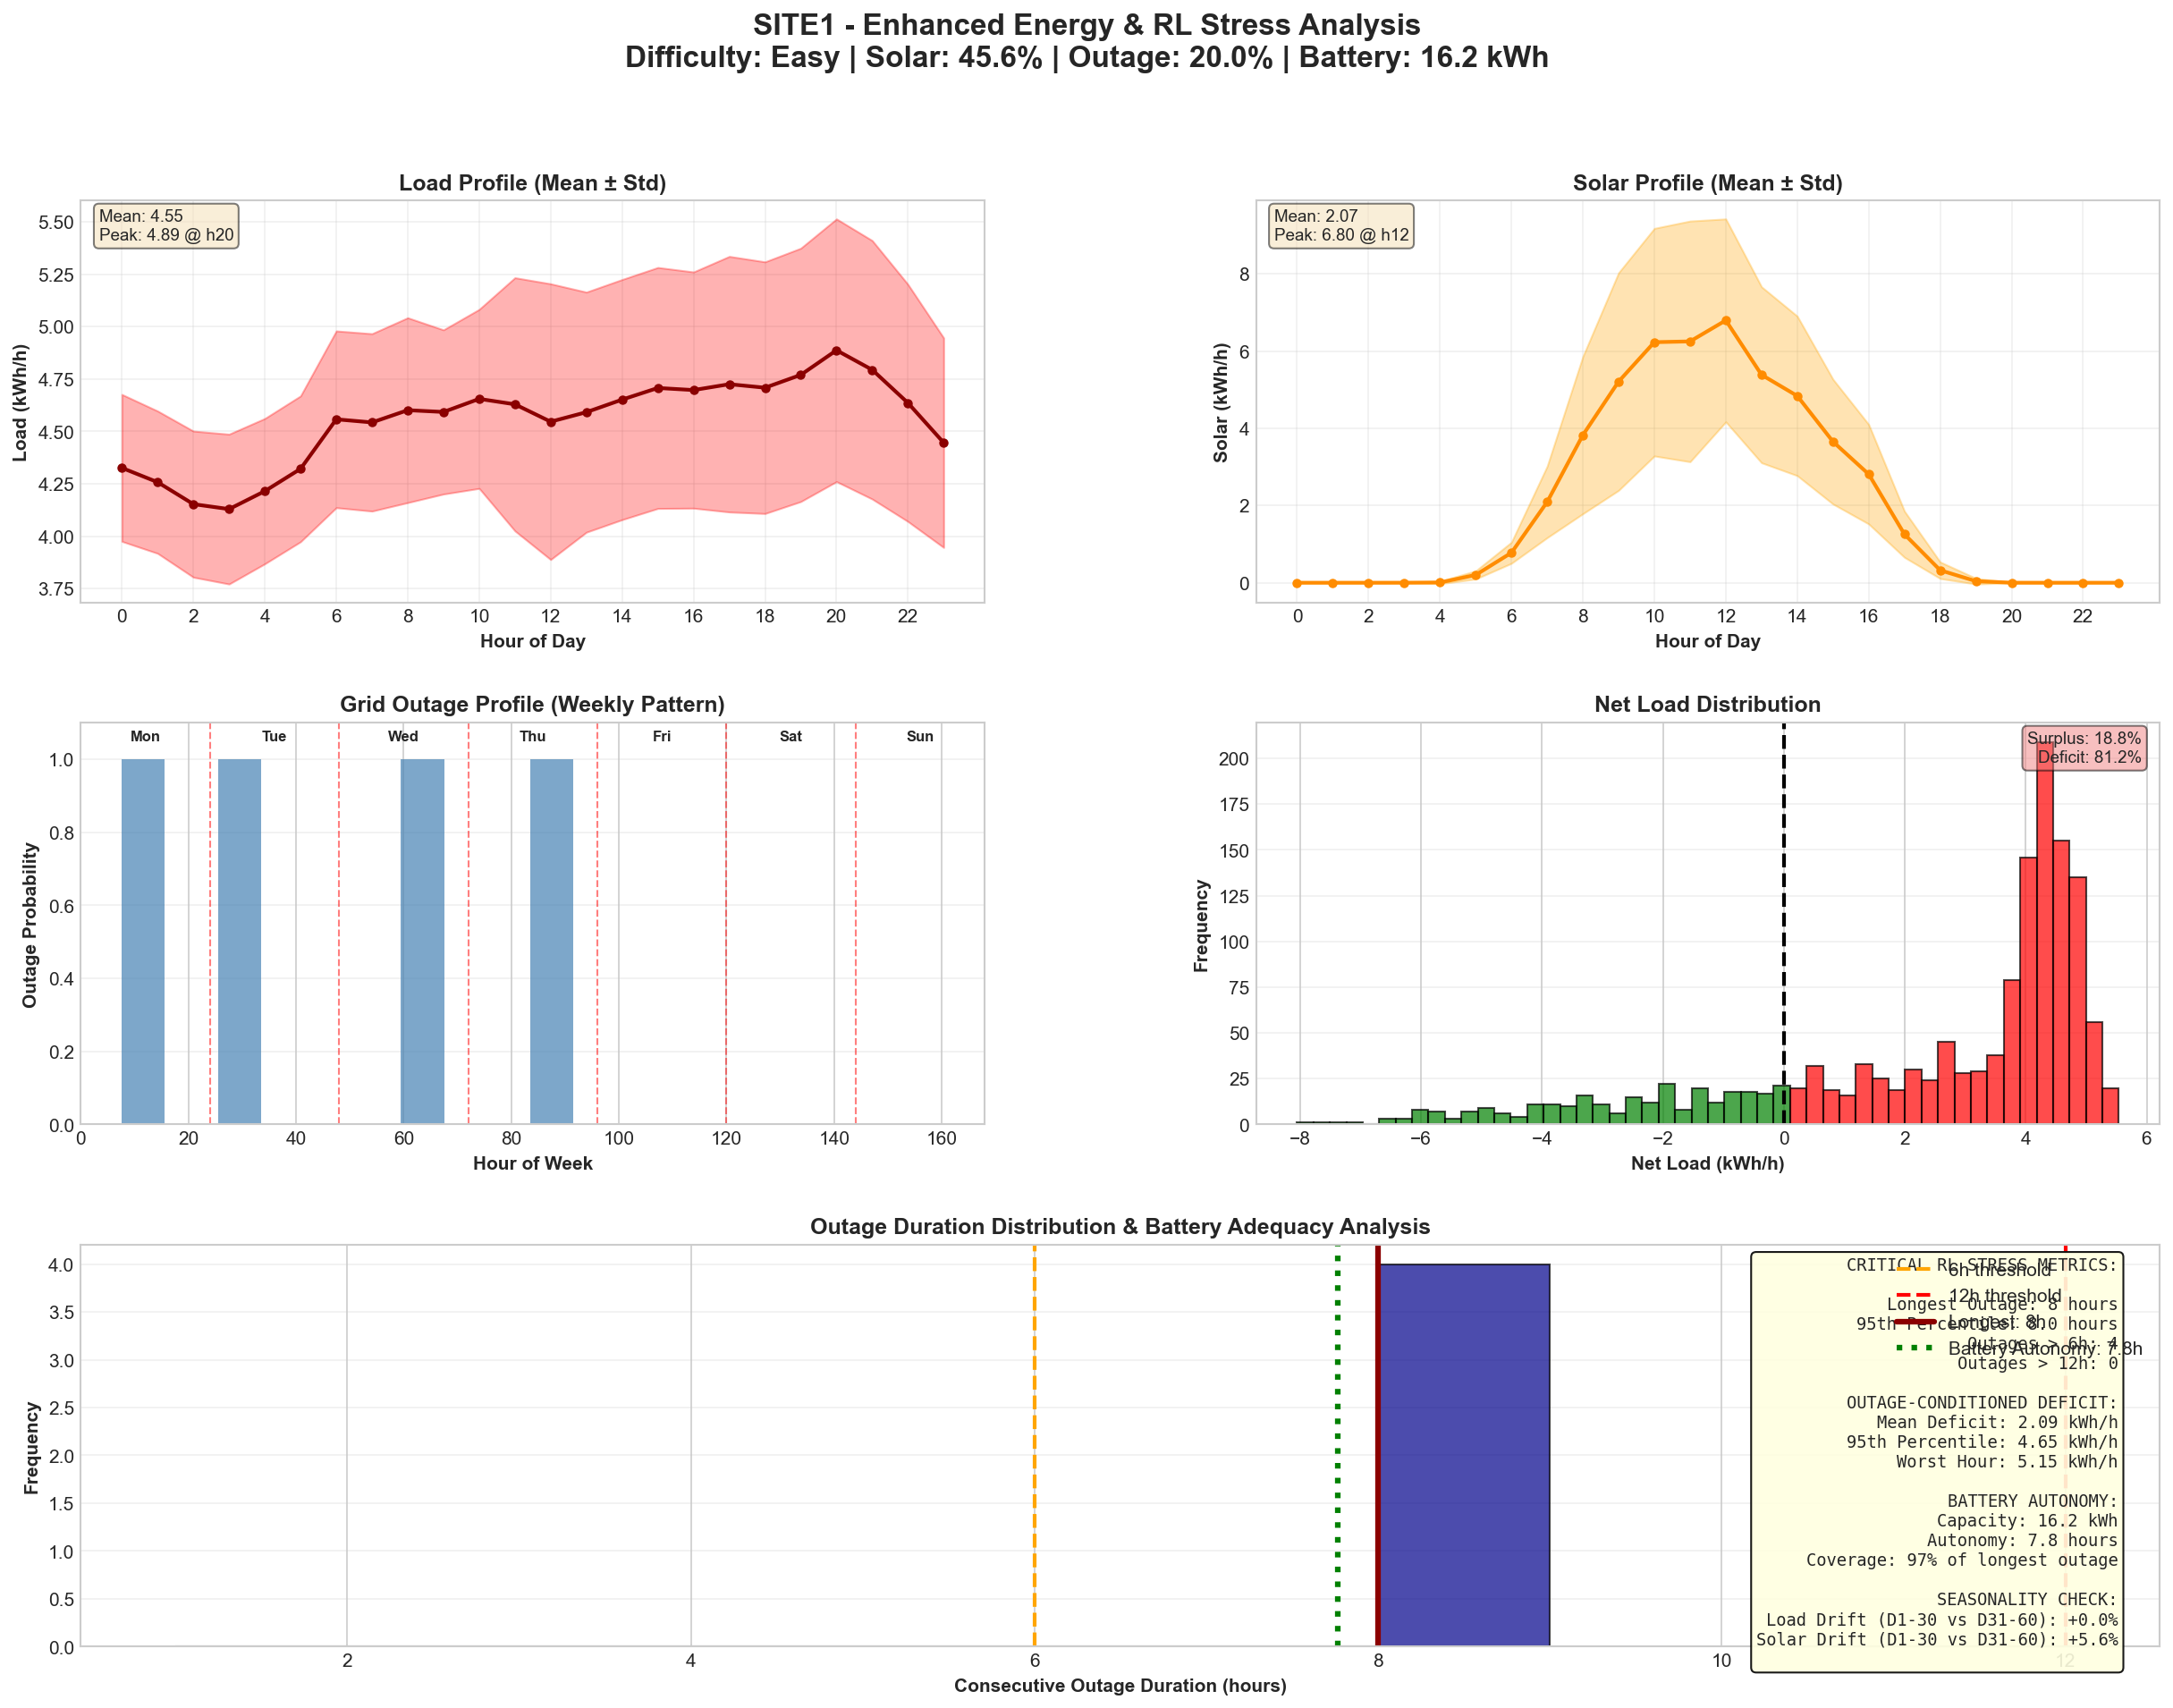
\includegraphics[width=\textwidth]{images/site1_enhanced_analysis}
\caption{Site~1 --- Easy. Load mean 4.55\,kWh/h; solar coverage 45.6\%;
grid availability 80.0\%; battery autonomy 7.8\,h (97\% of longest outage).
No outages exceed 12\,h. Outage-conditioned mean deficit 2.09\,kWh/h.}
\label{fig:app_site1}
\end{figure}

\begin{figure}[htbp]
\centering
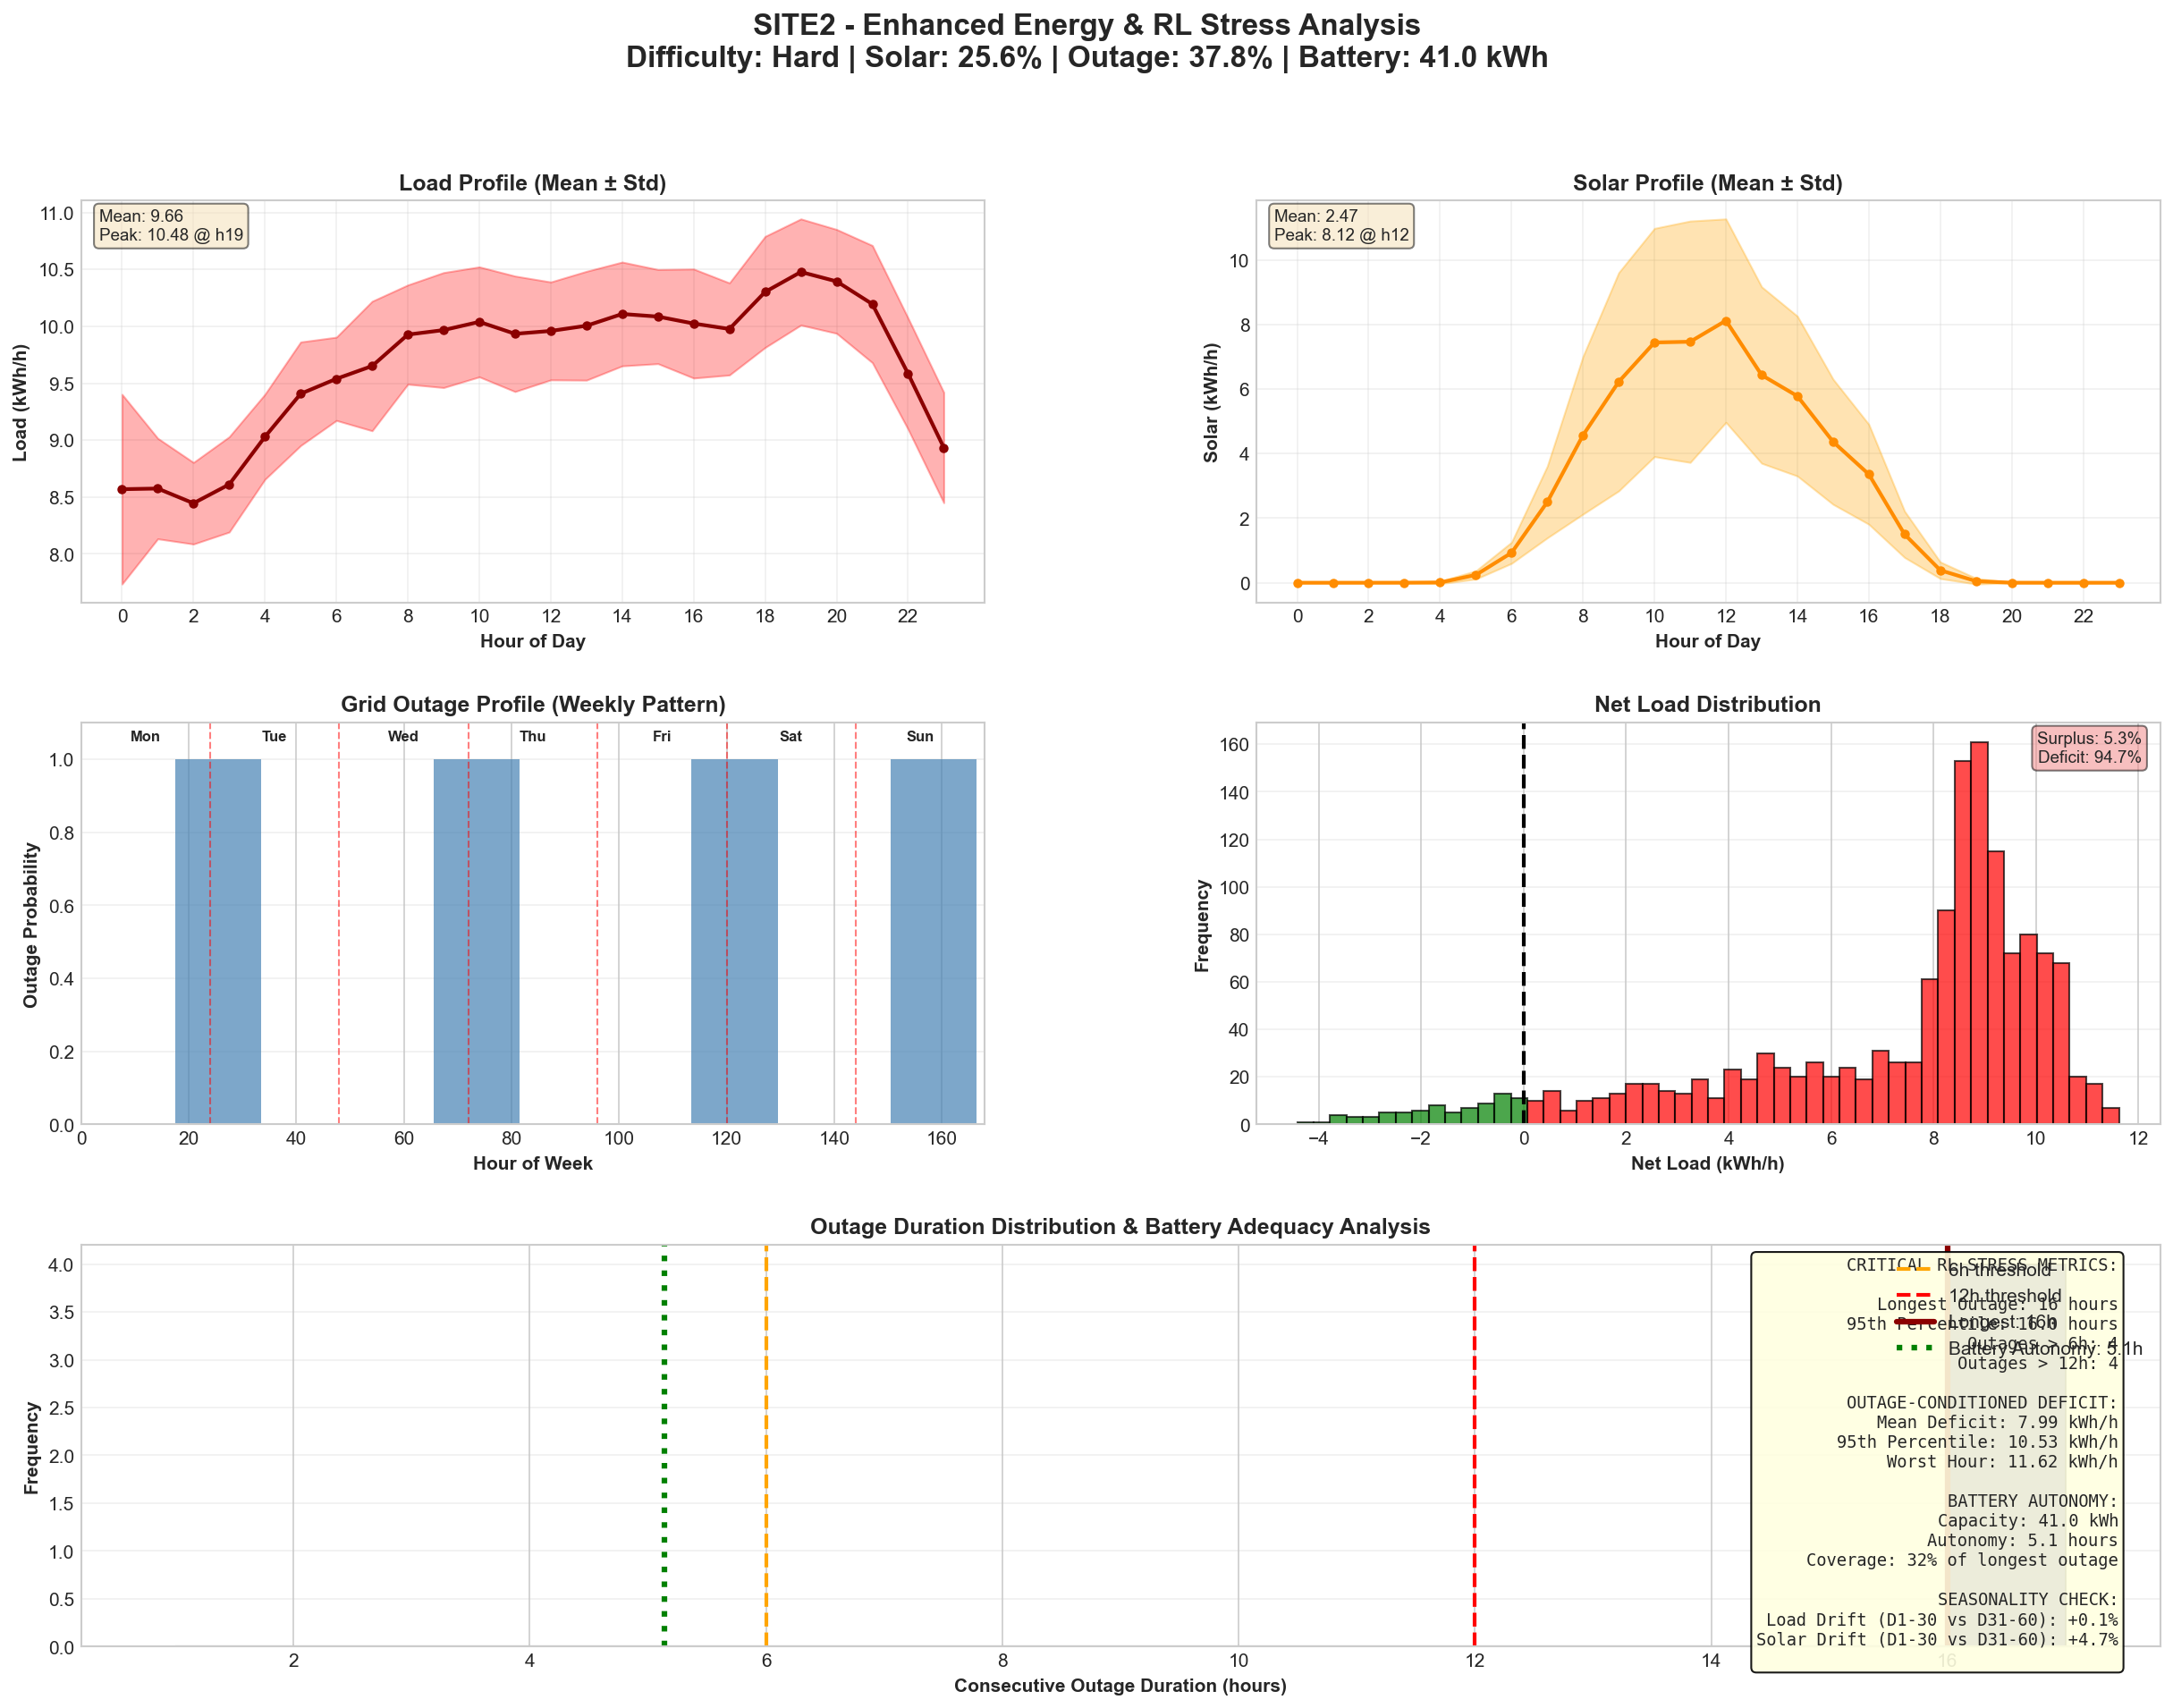
\includegraphics[width=\textwidth]{images/site2_enhanced_analysis}
\caption{Site~2 --- Hard. Load mean 9.66\,kWh/h (highest in dataset);
solar coverage 25.6\% (lowest); battery autonomy 5.1\,h (32\% of longest
outage). Four outages exceed 12\,h. Outage-conditioned mean deficit
7.99\,kWh/h.}
\label{fig:app_site2}
\end{figure}

\begin{figure}[htbp]
\centering
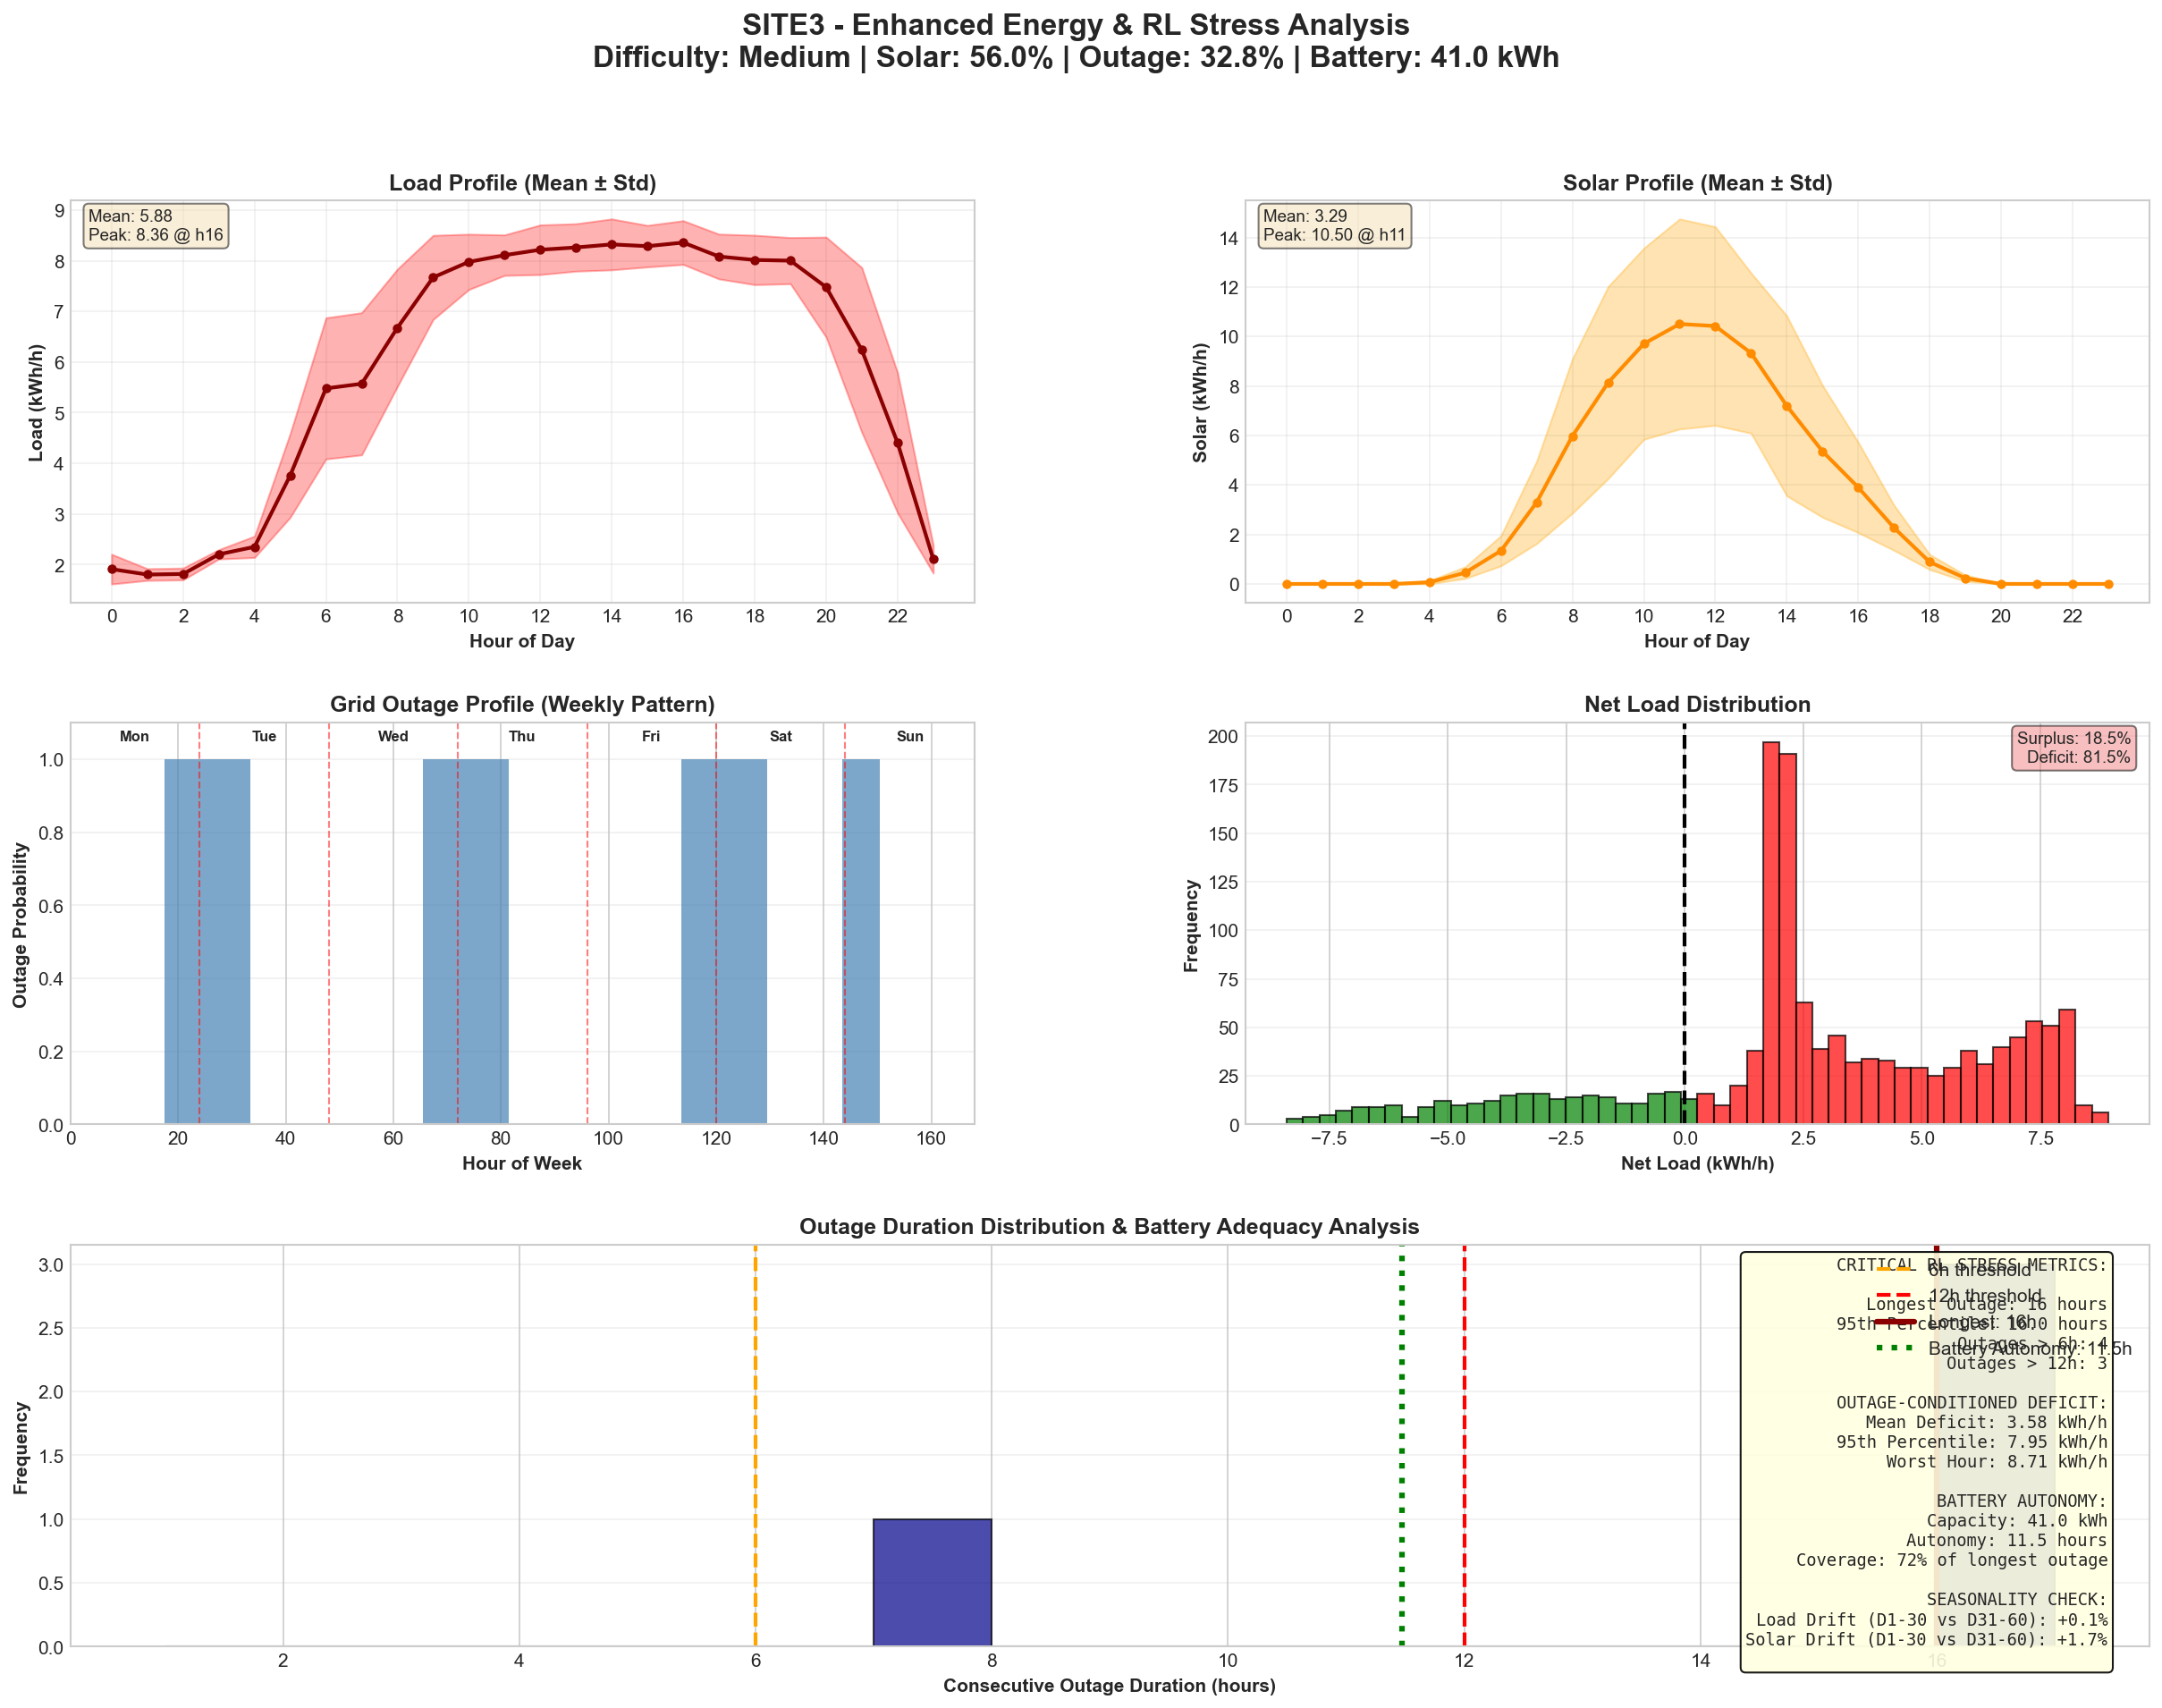
\includegraphics[width=\textwidth]{images/site3_enhanced_analysis}
\caption{Site~3 --- Medium. Load mean 5.88\,kWh/h; solar coverage 56.0\%;
battery autonomy 11.5\,h (72\% of longest outage). Three outages exceed
12\,h. Outage-conditioned mean deficit 3.58\,kWh/h.}
\label{fig:app_site3}
\end{figure}

\begin{figure}[htbp]
\centering
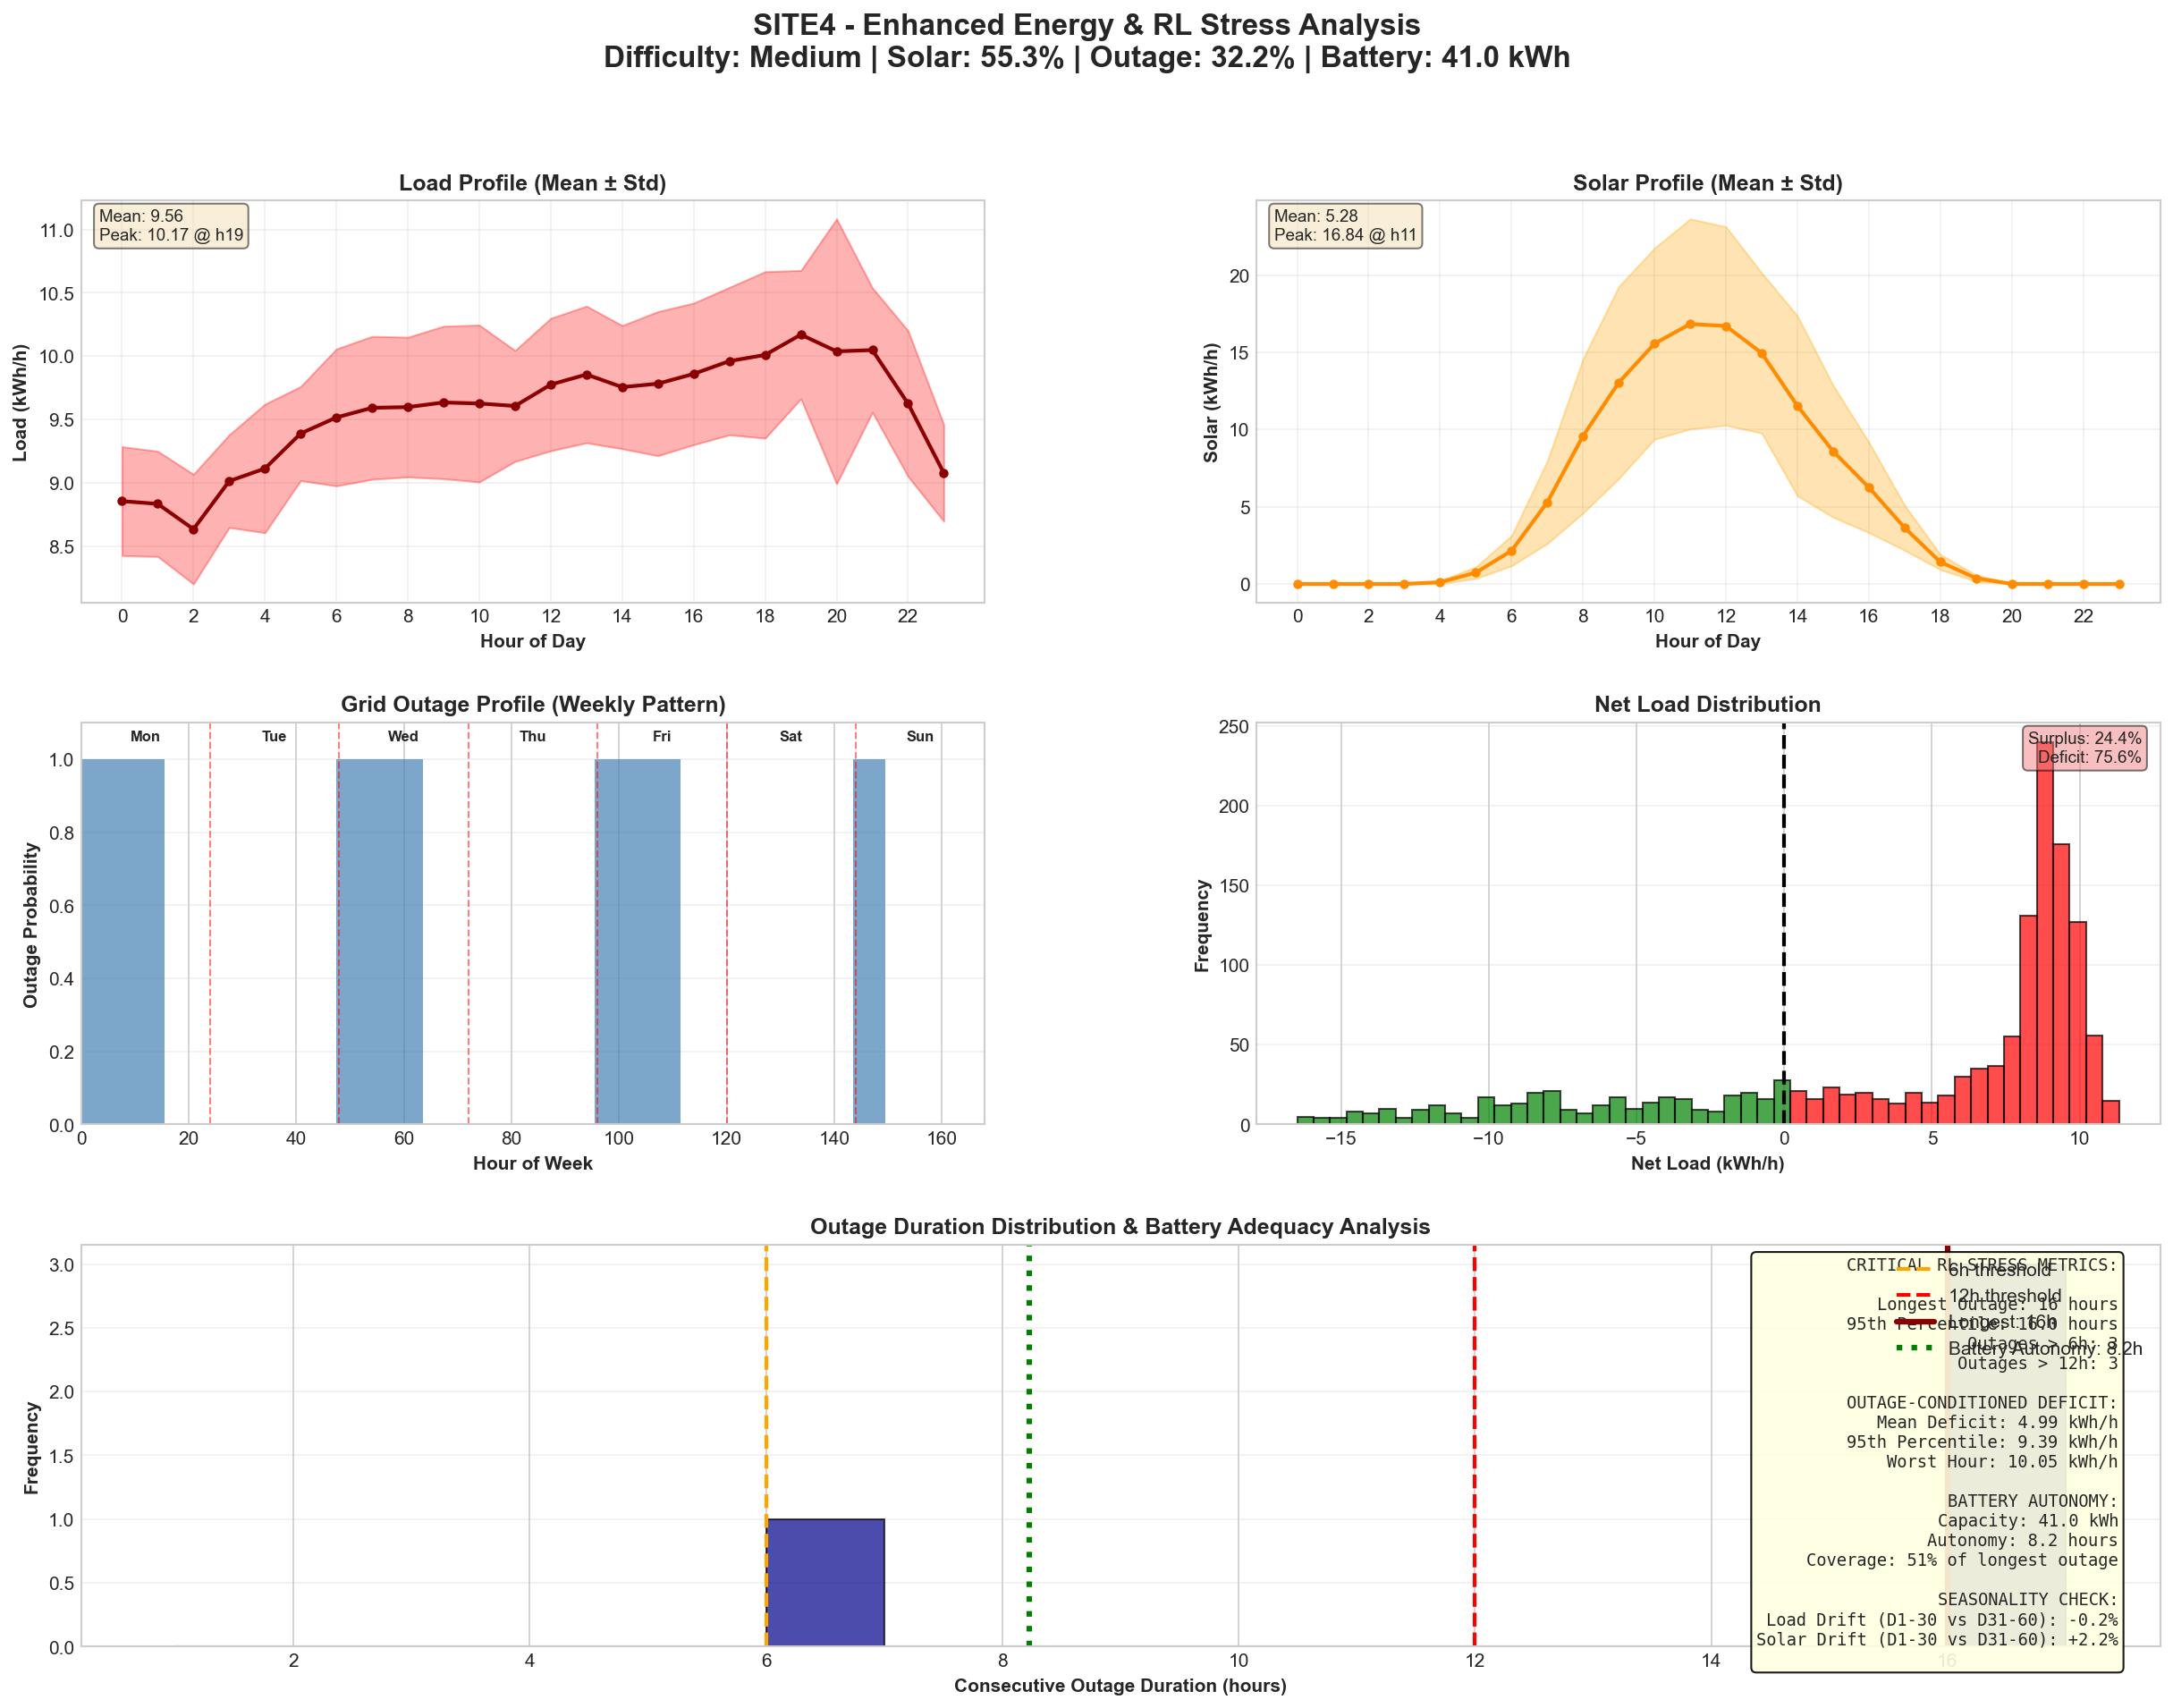
\includegraphics[width=\textwidth]{images/site4_enhanced_analysis}
\caption{Site~4 --- Medium. Load mean 9.56\,kWh/h; solar coverage 55.3\%;
battery autonomy 8.2\,h (51\% of longest outage). Three outages exceed
12\,h. Outage-conditioned mean deficit 4.99\,kWh/h. Notable for
combining high load with reasonable solar coverage.}
\label{fig:app_site4}
\end{figure}

\begin{figure}[htbp]
\centering
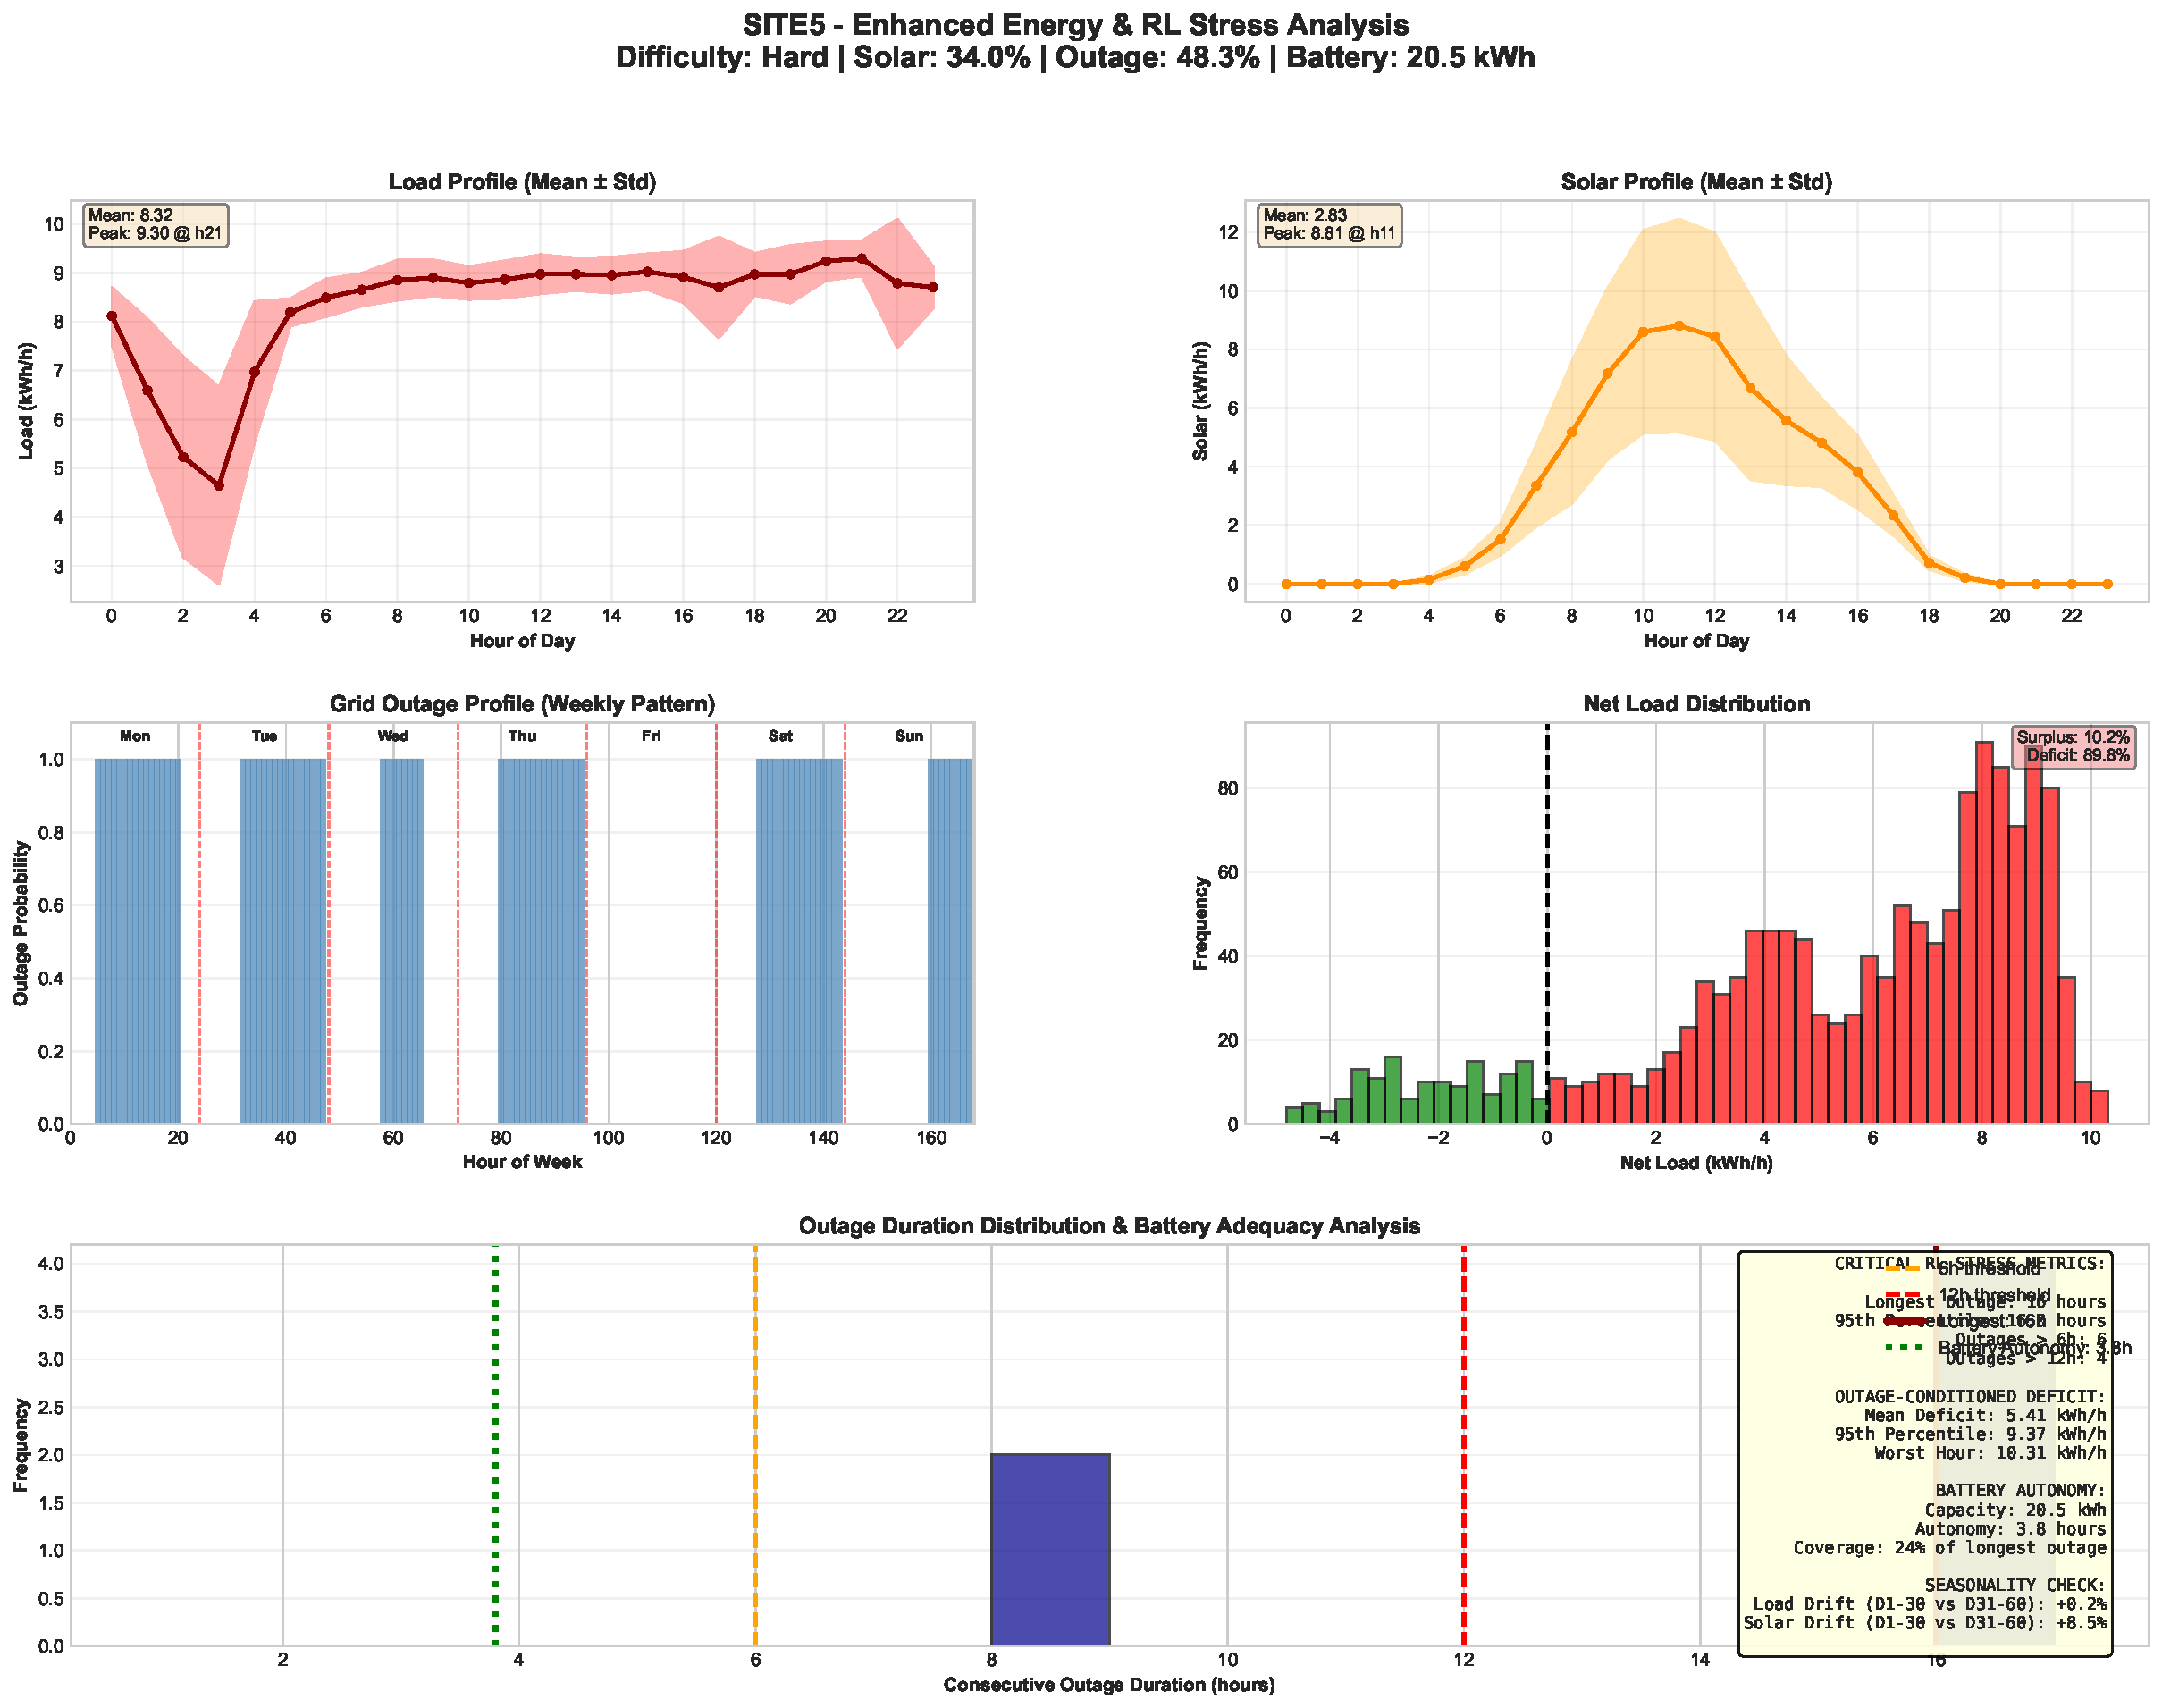
\includegraphics[width=\textwidth]{images/site5_enhanced_analysis}
\caption{Site~5 --- Hard. Load mean 8.32\,kWh/h; solar coverage 34.0\%;
battery autonomy 3.8\,h (24\% of longest outage). 52 outage events ---
highest frequency in dataset. Four outages exceed 12\,h.
Outage-conditioned mean deficit 5.41\,kWh/h.}
\label{fig:app_site5}
\end{figure}

\begin{figure}[htbp]
\centering
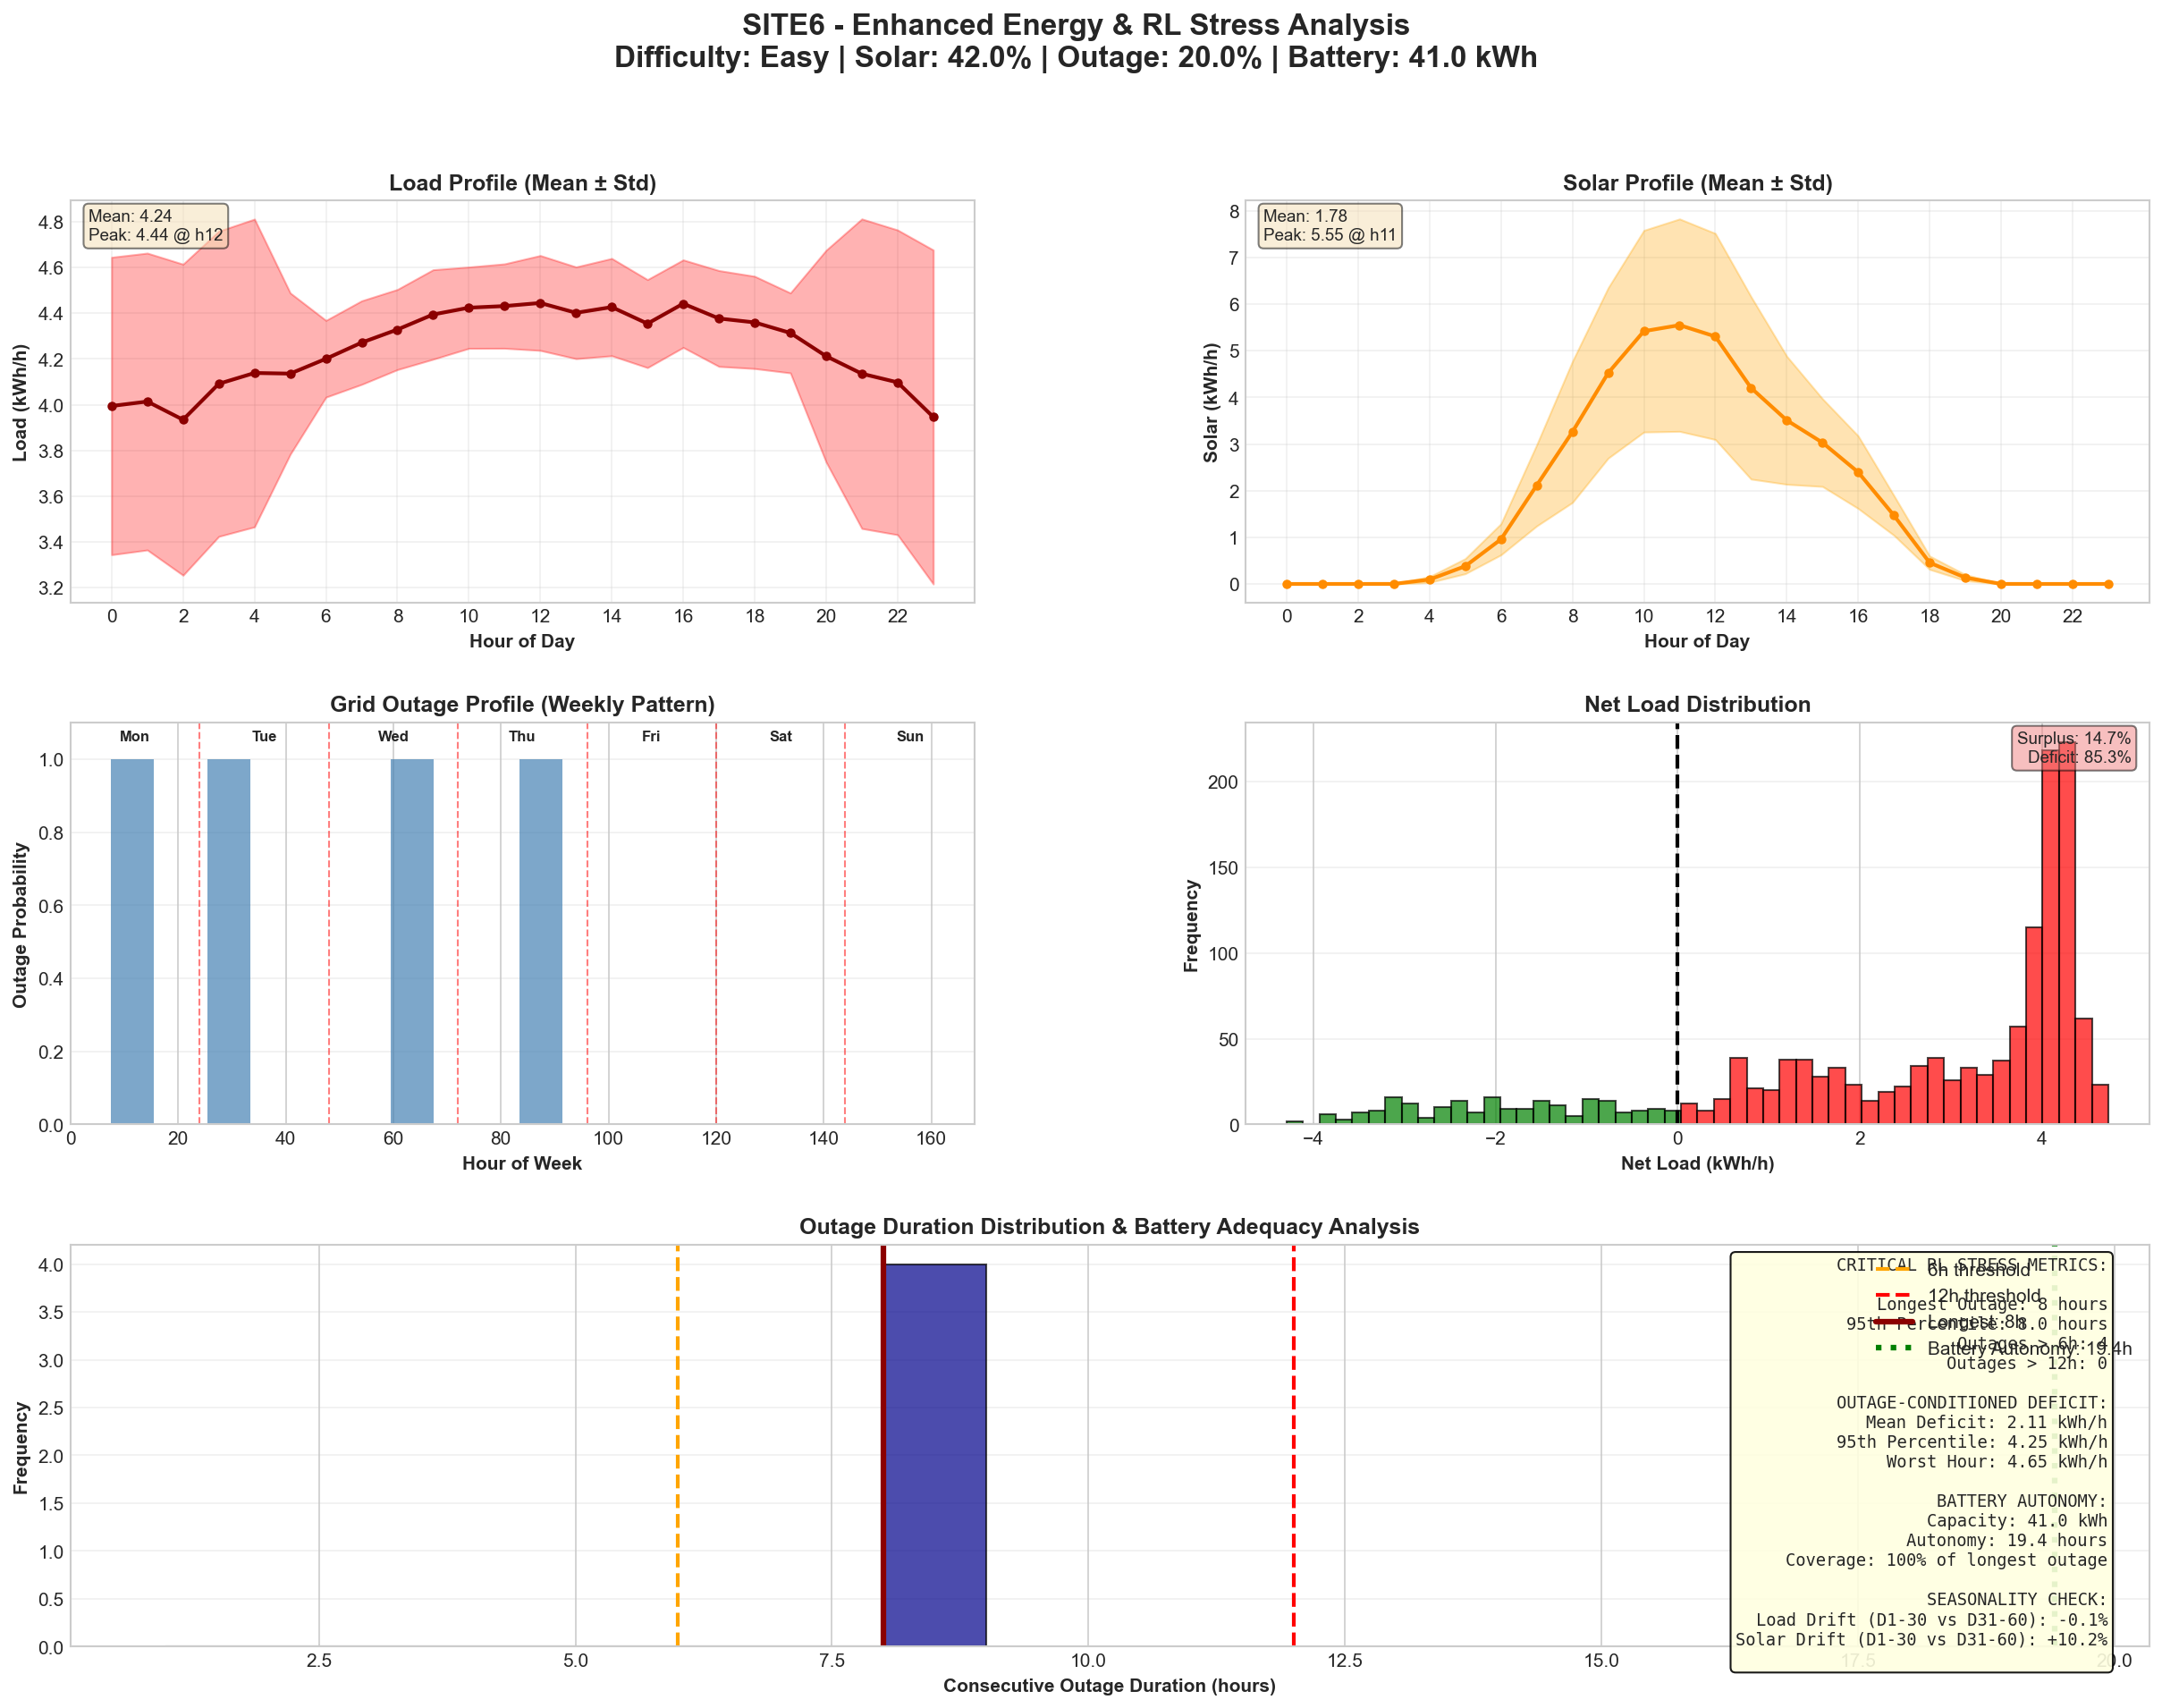
\includegraphics[width=\textwidth]{images/site6_enhanced_analysis}
\caption{Site~6 --- Easy. Load mean 4.24\,kWh/h; solar coverage 42.0\%;
grid availability 80.0\%; battery autonomy 19.4\,h (100\% of longest
outage). No outages exceed 12\,h. Outage-conditioned mean deficit
2.11\,kWh/h. Site~6 is the most battery-adequate site in the dataset.}
\label{fig:app_site6}
\end{figure}

\begin{figure}[htbp]
\centering
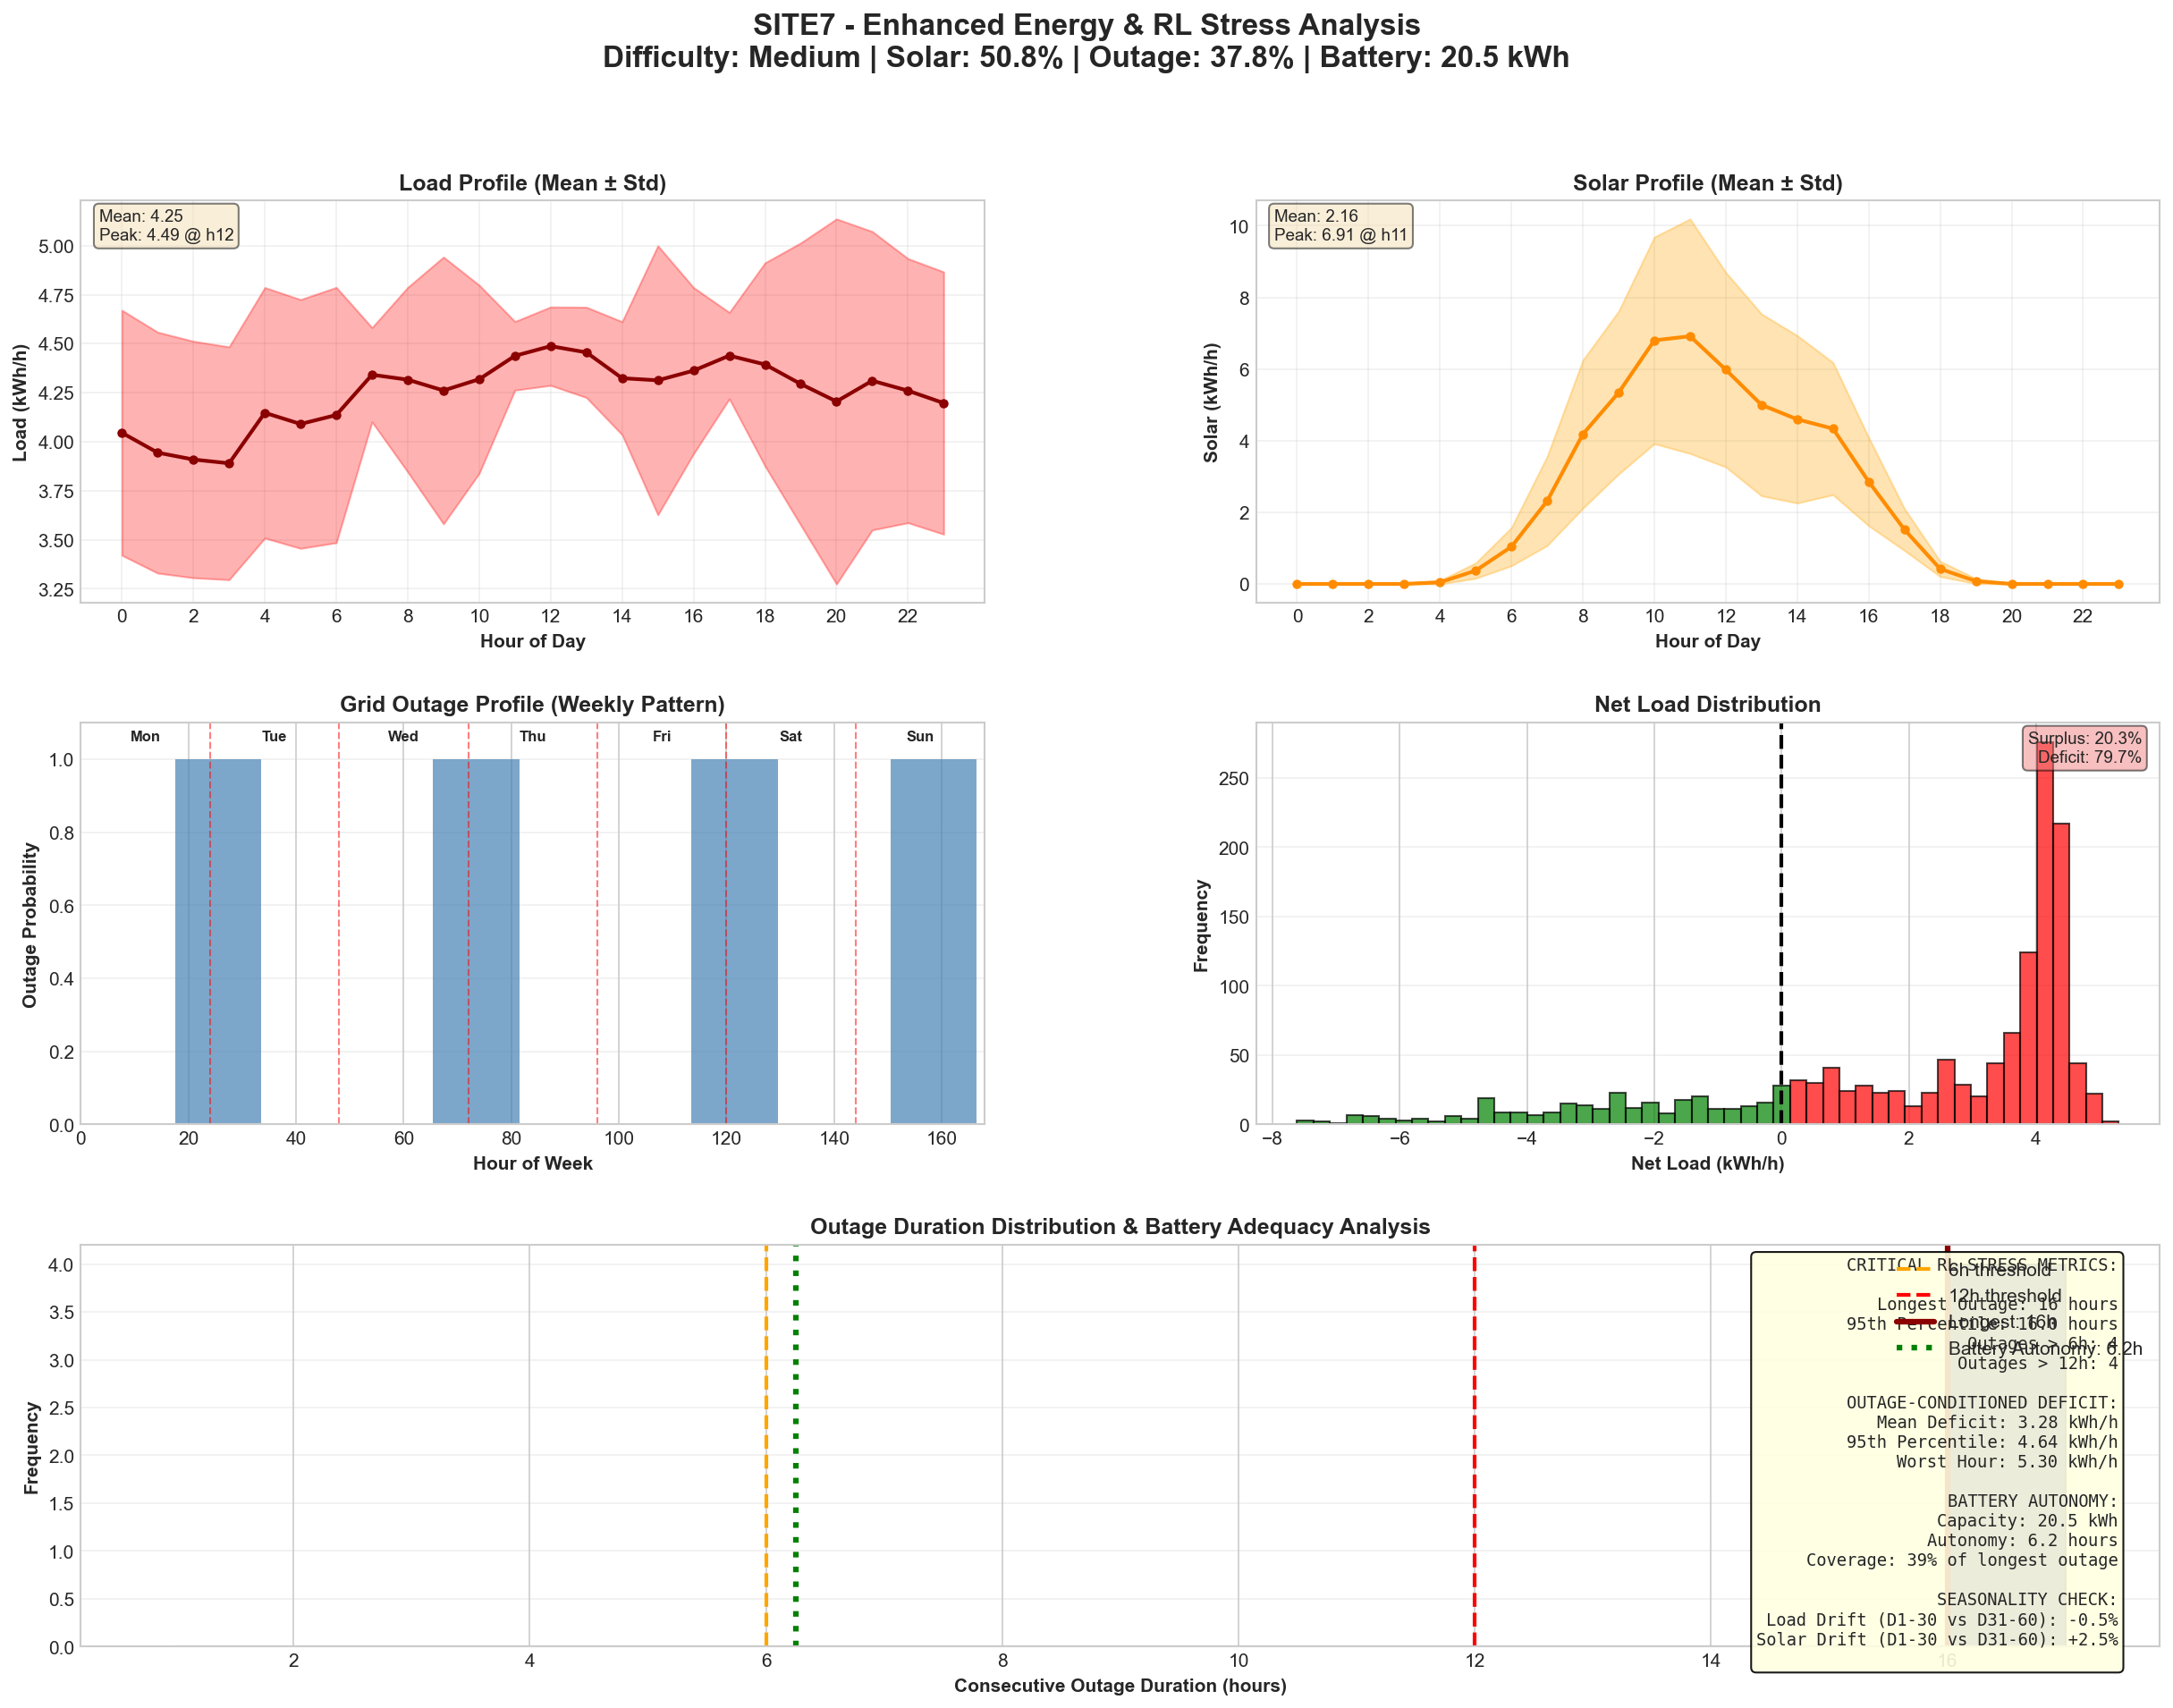
\includegraphics[width=\textwidth]{images/site7_enhanced_analysis}
\caption{Site~7 --- Medium. Load mean 4.25\,kWh/h; solar coverage 50.8\%;
battery autonomy 6.2\,h (39\% of longest outage). Four outages exceed
12\,h. Outage-conditioned mean deficit 3.28\,kWh/h. Despite moderate
load, battery undersizing relative to 16-hour outages creates reliability
risk.}
\label{fig:app_site7}
\end{figure}

\begin{figure}[htbp]
\centering
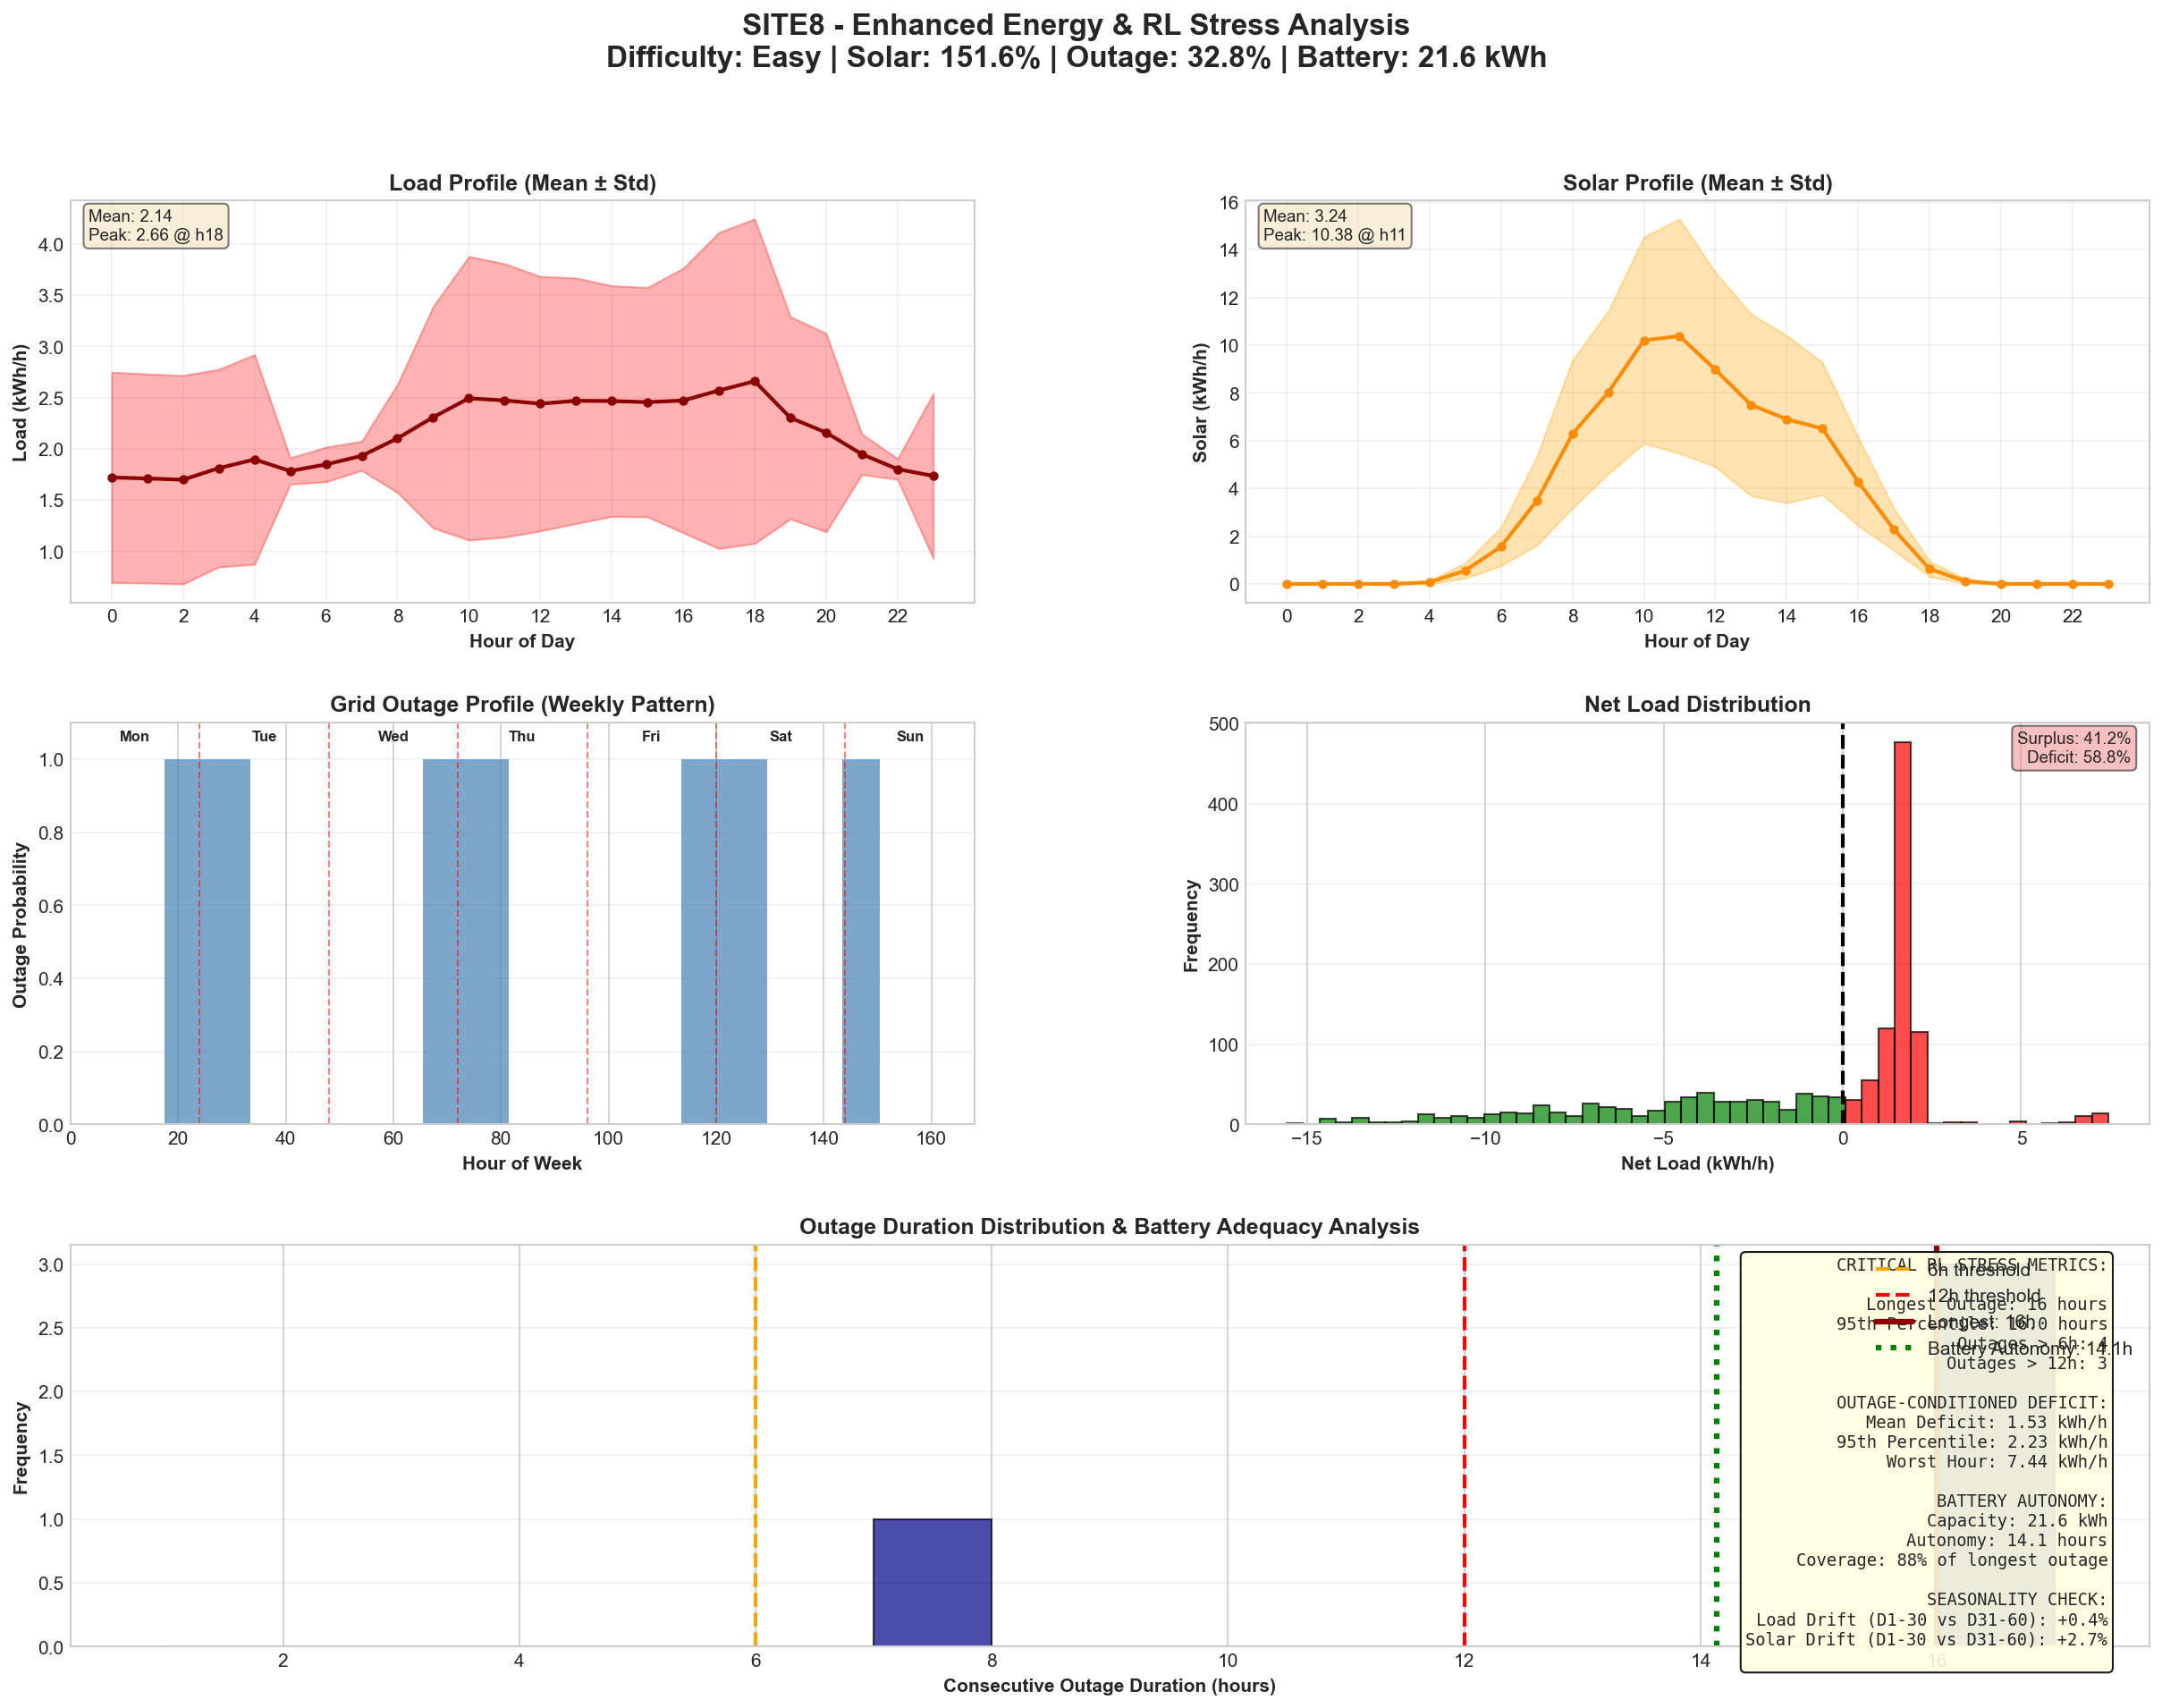
\includegraphics[width=\textwidth]{images/site8_enhanced_analysis}
\caption{Site~8 --- Easy (solar surplus). Load mean 2.14\,kWh/h; solar
coverage 151.6\%; battery autonomy 14.1\,h (88\% of longest outage).
41.2\% of hours are solar-surplus. Three outages exceed 12\,h but
outage-conditioned mean deficit is only 1.53\,kWh/h. Primary challenge
is battery saturation and curtailment, not stockout.}
\label{fig:app_site8}
\end{figure}

\begin{figure}[htbp]
\centering
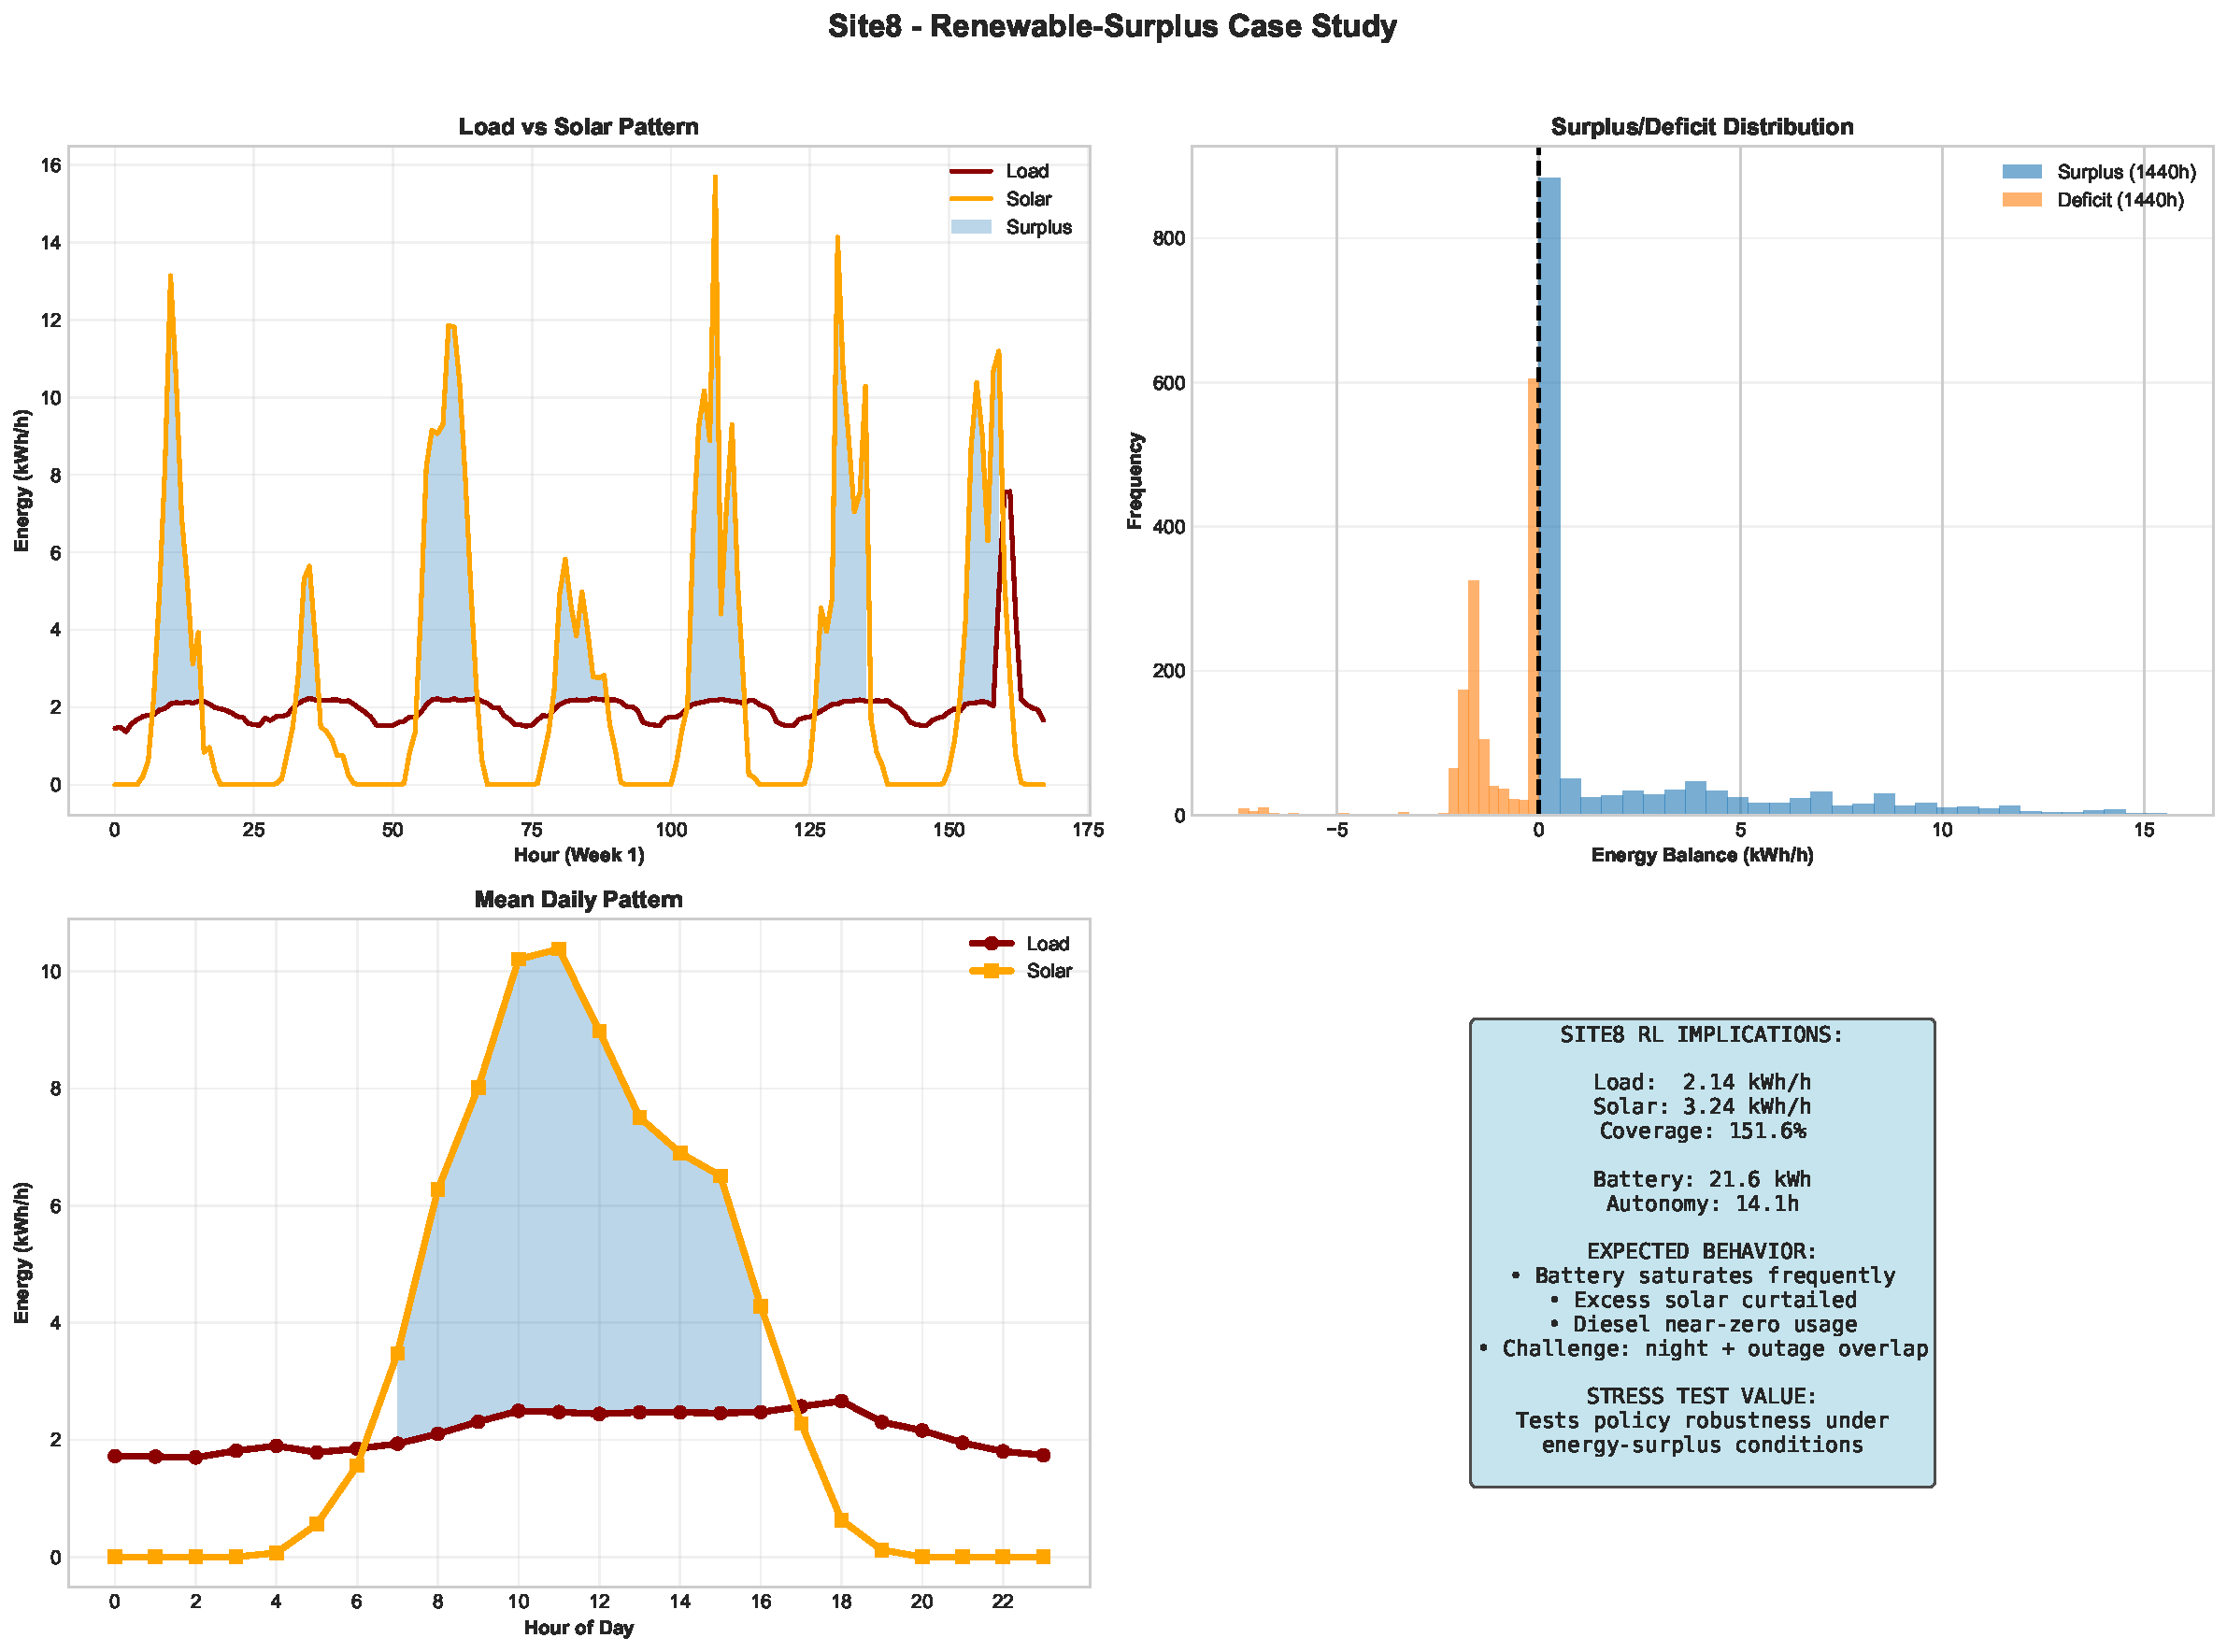
\includegraphics[width=\textwidth]{images/fig3_site8_surplus}
\caption{Site~8 renewable-surplus case study showing load vs.\ solar time
series (top-left), surplus/deficit distribution (top-right), and mean
daily pattern (bottom-left). 41\% of hours are solar-surplus; average
surplus 51\,kWh/day.}
\label{fig:app_site8_surplus}
\end{figure}

\begin{figure}[htbp]
\centering
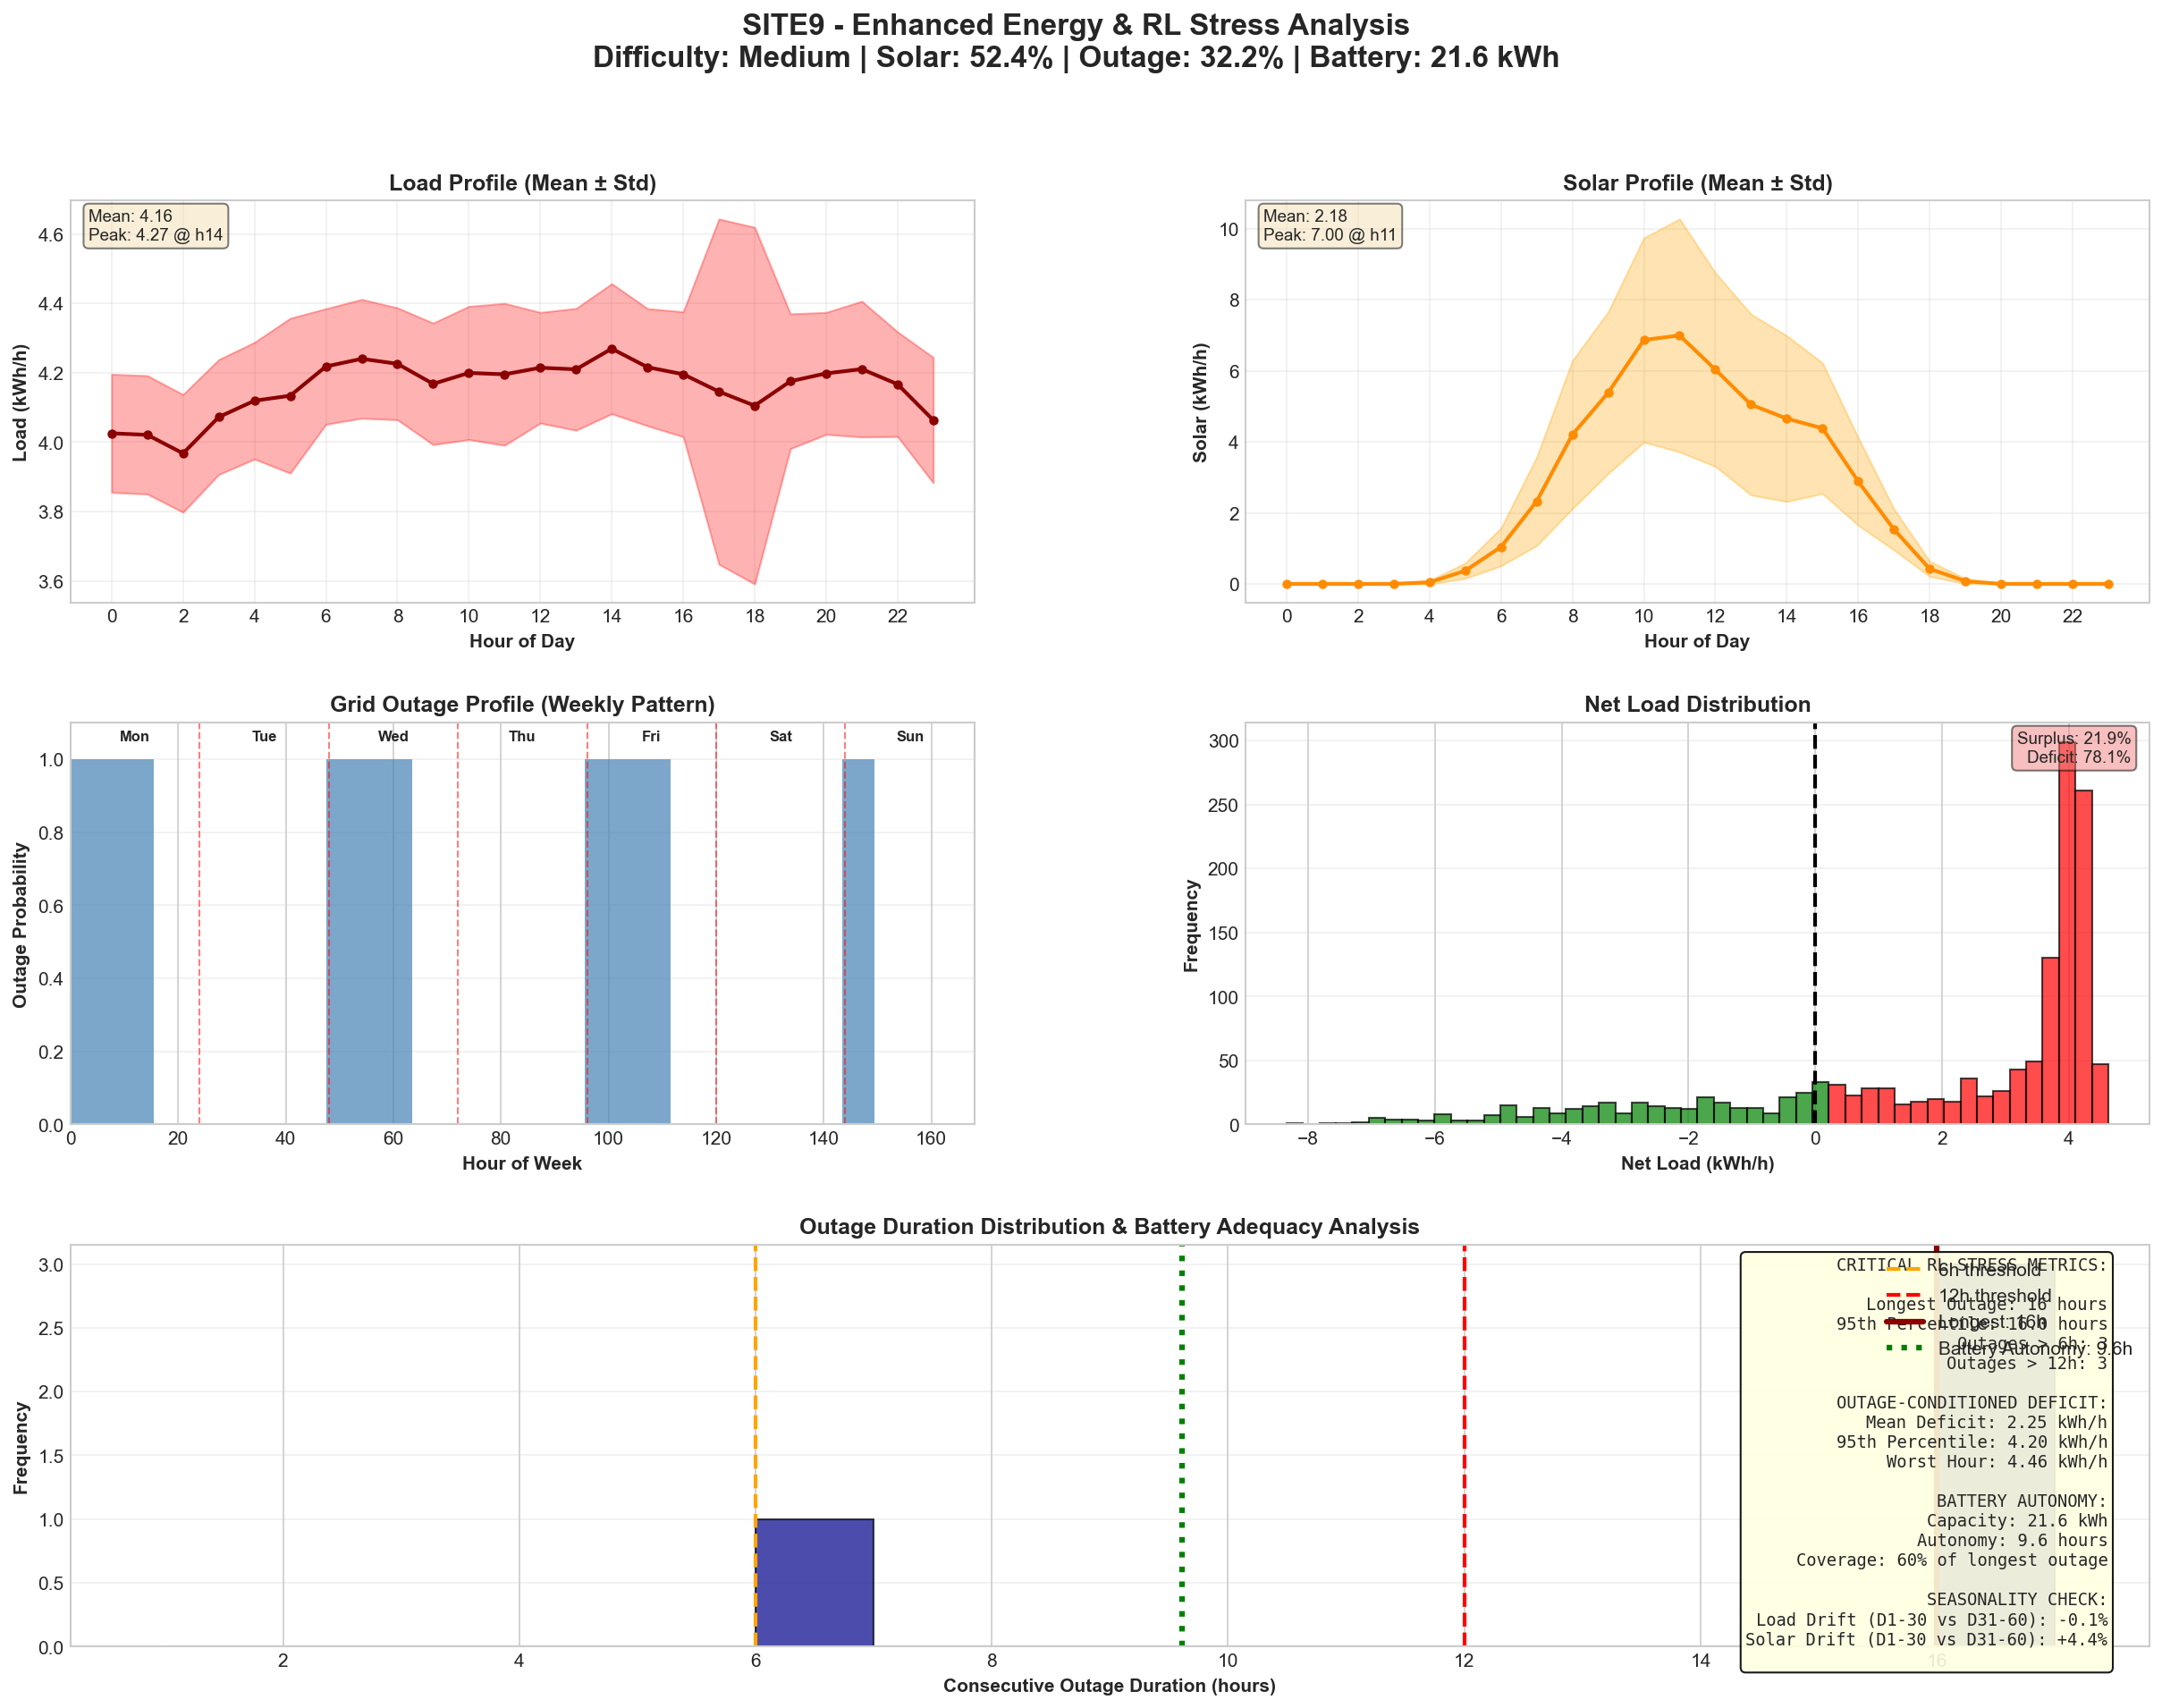
\includegraphics[width=\textwidth]{images/site9_enhanced_analysis}
\caption{Site~9 --- Medium. Load mean 4.16\,kWh/h; solar coverage 52.4\%;
battery autonomy 9.6\,h (60\% of longest outage). Three outages exceed
12\,h. Outage-conditioned mean deficit 2.25\,kWh/h. Moderate difficulty
across all dimensions.}
\label{fig:app_site9}
\end{figure}

\begin{figure}[htbp]
\centering
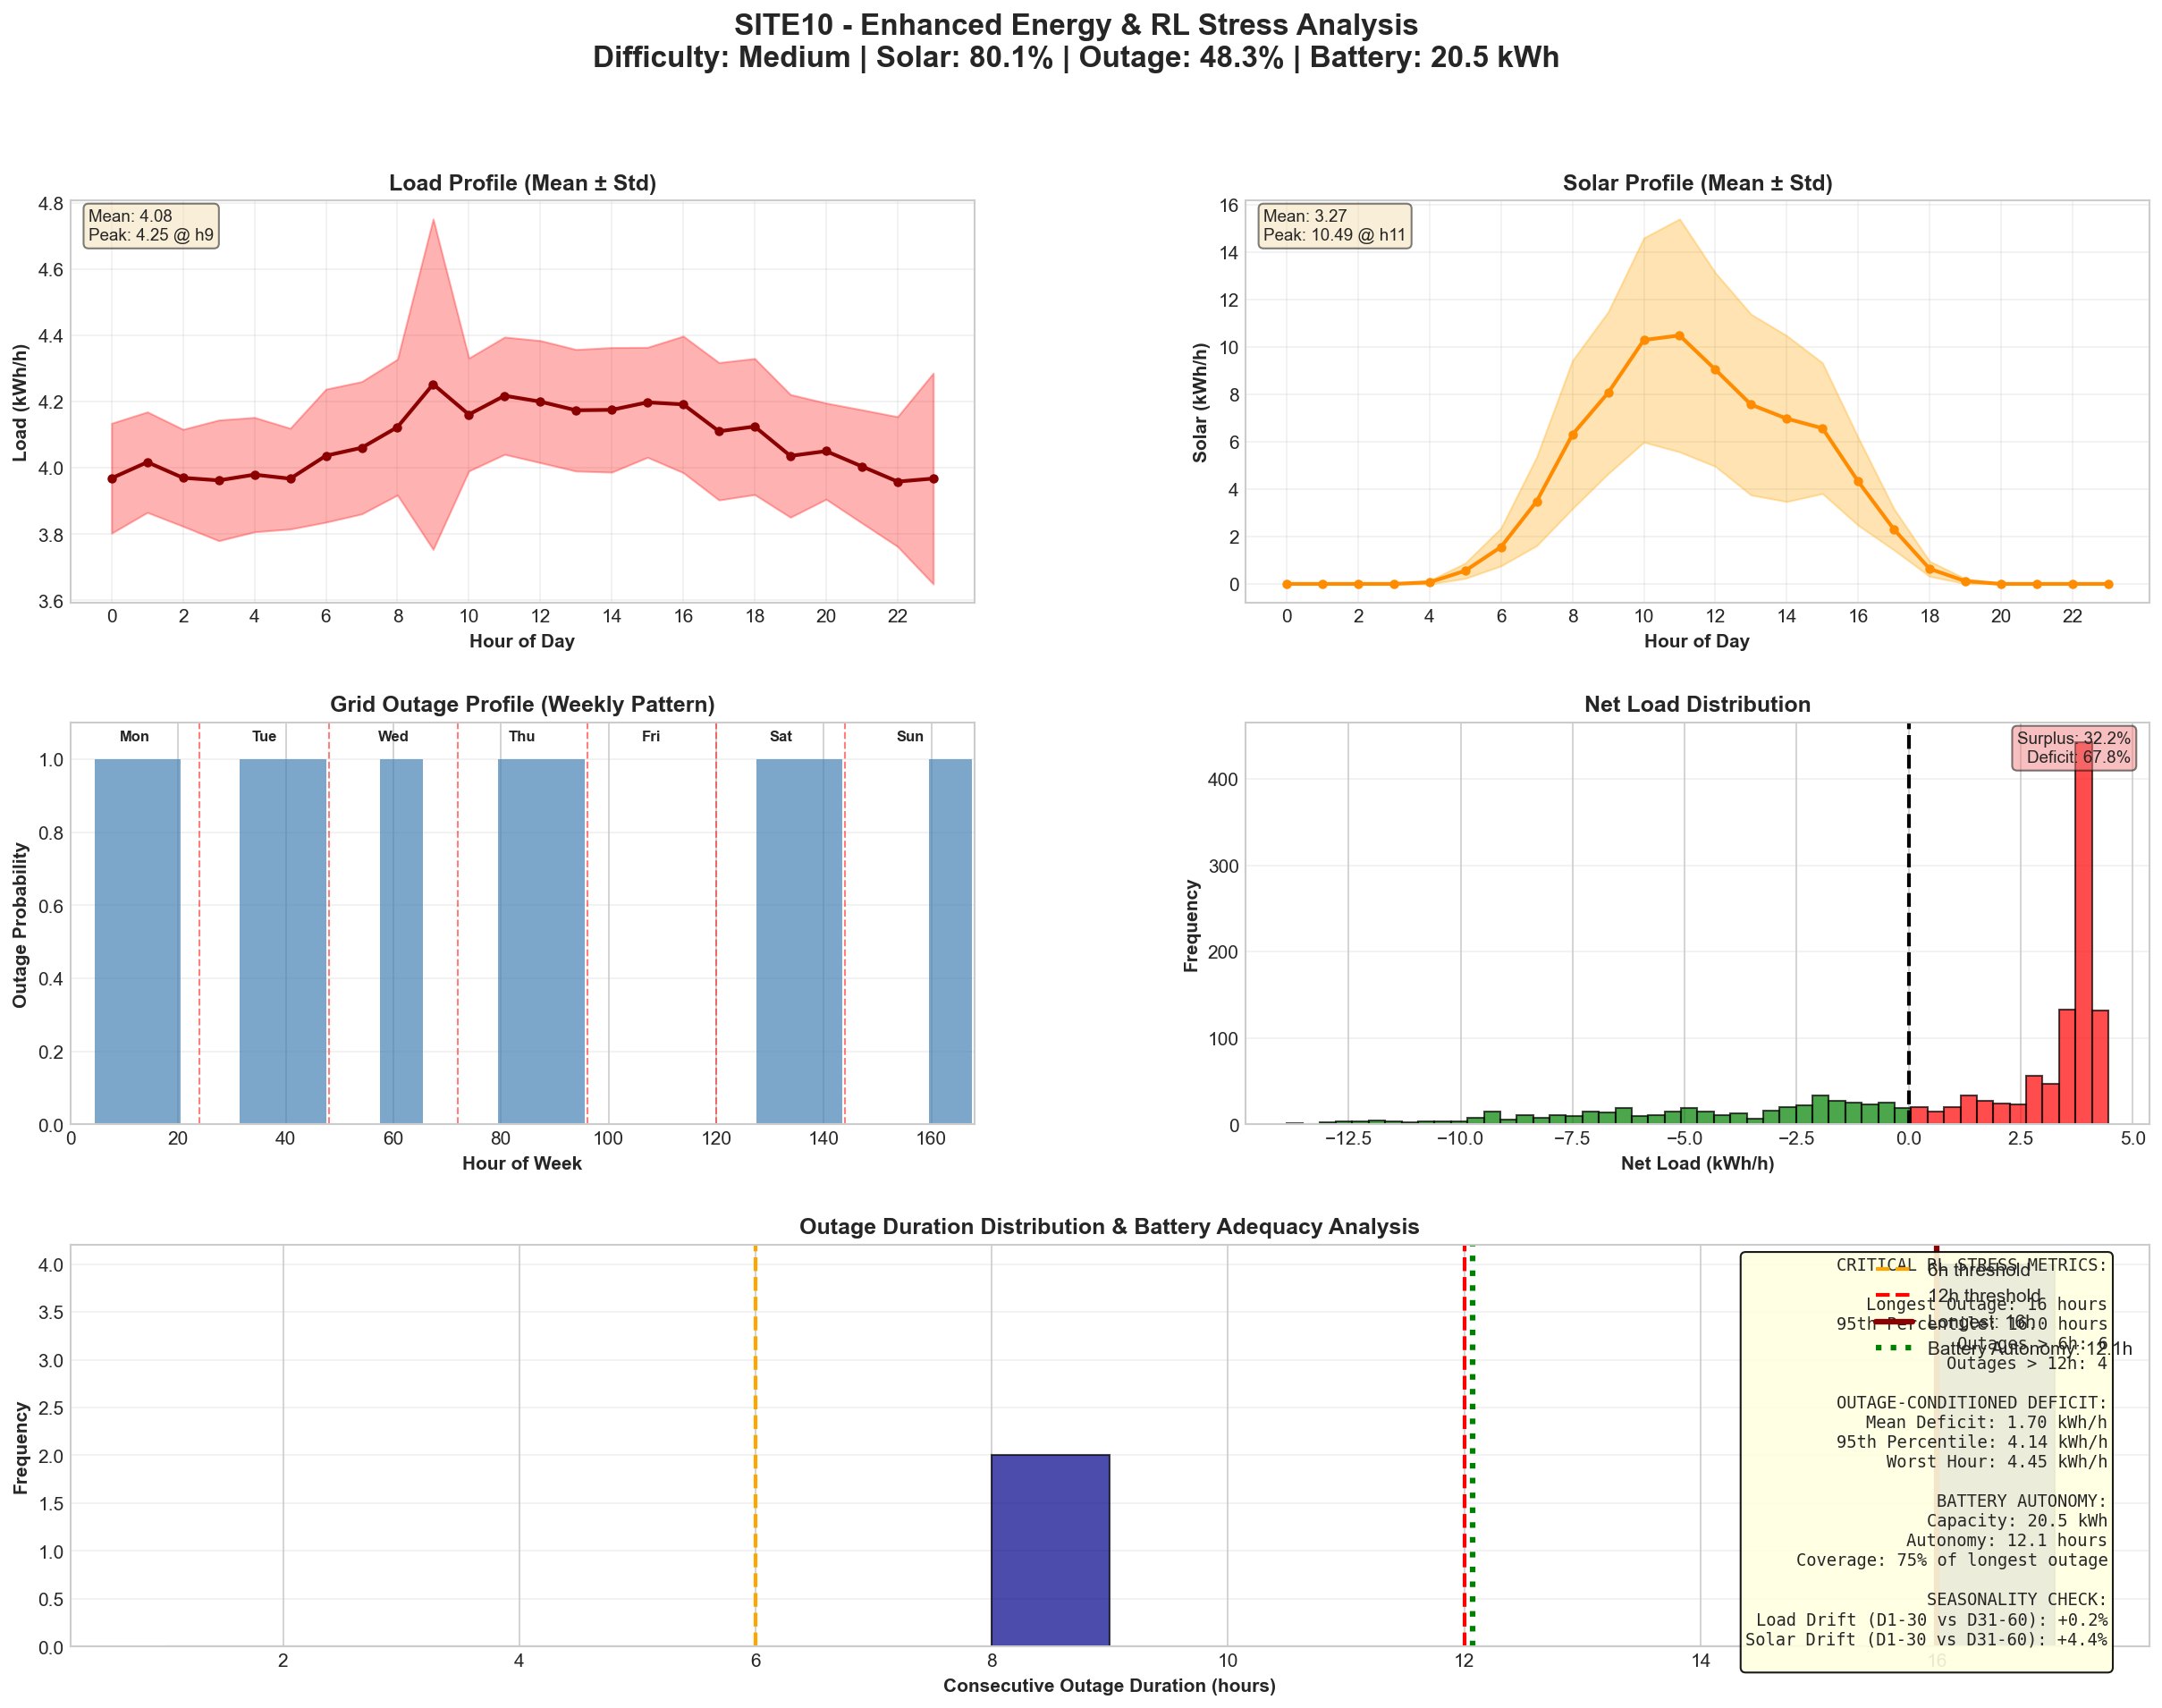
\includegraphics[width=\textwidth]{images/site10_enhanced_analysis}
\caption{Site~10 --- Medium (delayed-scenario edge case). Load mean
4.08\,kWh/h; solar coverage 80.1\%; battery autonomy 12.1\,h (75\% of
longest outage). Four outages exceed 12\,h. Despite a moderate composite score, high outage frequency (48.3\%)
combined with outages approaching battery autonomy makes this site
sensitive to logistics delays.}
\label{fig:app_site10}
\end{figure}  
    \chapter[Supplementary Training-Budget Analysis]
    {\revised{Supplementary Training-Budget Analysis}}
    \label{app:rl_training_budget}
    
% ============================================================
% Supplementary Training-Budget Analysis
% ============================================================

\begin{revisedblock}
This appendix provides supplementary results on the
sensitivity of DQN and A2C reliability to training
budget. Intermediate model checkpoints corresponding
to nominal budgets of 50,000, 100,000, and 200,000
interactions were evaluated alongside the final
400,000-interaction checkpoints.

The evaluation used site1, site3, and site5, five
independent training seeds, four supplier-delay
scenarios, and ten evaluation episodes per seed and
scenario. The intermediate-checkpoint analysis
comprised 90 model evaluations and 3,600 held-out
episodes. Each checkpoint was evaluated using its
corresponding saved observation-normalisation
statistics.

Table~\ref{tab:appendix_rl_budget} reports the
results for site5, where reliability differences
were most evident. Mean EENS is calculated across
five training seeds and four delivery scenarios.

Differences are measured relative to the final
checkpoint. The exploratory 95\% confidence
intervals are based on paired training-seed results.
\end{revisedblock}


\begin{table}[htbp]
\centering
\small
\caption{\revised{Training-budget sensitivity for
DQN and A2C on site5. Mean EENS and differences
are in kWh per 360-hour episode. A positive
difference indicates higher EENS than the final
checkpoint.}}
\label{tab:appendix_rl_budget}
\begin{tabular}{llrrl}
\toprule
\textbf{Algorithm} &
\textbf{Budget} &
\textbf{Mean EENS} &
\textbf{Difference} &
\textbf{95\% CI} \\
\midrule
\revised{DQN} & \revised{50k} &
\revised{84.8580} & \revised{+3.9729} &
\revised{$[-3.2409,\ 11.1866]$} \\
\revised{DQN} & \revised{100k} &
\revised{81.0724} & \revised{+0.1872} &
\revised{$[-1.0218,\ 1.3963]$} \\
\revised{DQN} & \revised{200k} &
\revised{80.9840} & \revised{+0.0988} &
\revised{$[-0.9470,\ 1.1447]$} \\
\revised{DQN} & \revised{400k} &
\revised{80.8852} & \revised{--} &
\revised{Reference} \\
\midrule
\revised{A2C} & \revised{50k} &
\revised{83.7292} & \revised{-1.0674} &
\revised{$[-2.6841,\ 0.5492]$} \\
\revised{A2C} & \revised{100k} &
\revised{84.3715} & \revised{-0.4252} &
\revised{$[-2.3601,\ 1.5097]$} \\
\revised{A2C} & \revised{200k} &
\revised{84.0428} & \revised{-0.7539} &
\revised{$[-2.4176,\ 0.9099]$} \\
\revised{A2C} & \revised{400k} &
\revised{84.7967} & \revised{--} &
\revised{Reference} \\
\bottomrule
\end{tabular}
\end{table}

\begin{revisedblock}
For DQN, mean EENS on site5 decreases from
84.8580 kWh at 50,000 interactions to
81.0724 kWh at 100,000, followed by smaller
numerical improvements at subsequent checkpoints.
A2C does not exhibit a consistent improvement
with additional interactions.

Across all three sites, four delivery scenarios,
and three intermediate checkpoints, none of the
72 exploratory paired 95\% confidence intervals
for EENS differences relative to the final
checkpoint excludes zero. Site1 records zero
EENS for both algorithms at all checkpoints,
while site3 provides limited additional
discrimination.

These results describe training-budget sensitivity
rather than statistically established convergence.
The final 400,000-interaction checkpoints were
retained for the main algorithm comparison;
intermediate checkpoints were not selected based
on held-out evaluation performance.

Equivalent intermediate-checkpoint evaluations
were not available for the historical RLInv and A7
models. Consequently, this supplementary analysis
does not establish relative learning efficiency
across all four RL algorithms.
\end{revisedblock}

  \end{MainMatter}

  % ============== BACK MATTER (references etc.) ===================
  \begin{BackMatter}
    \printBibliographyReferences{references}
    % \printCV
    % \printCommittee
  \end{BackMatter}

\end{document}